\documentclass[a4paper, 12pt, oneside]{book}
\pagestyle{empty}
\usepackage[spanish]{babel}  % 
\usepackage[a4paper, left=2.5cm, right=2.5cm, top=3cm, bottom=3cm]{geometry}
\usepackage{times}
\usepackage{caption}
\usepackage{tablefootnote}
\usepackage{subcaption}
\usepackage[utf8]{inputenc} 
\usepackage{fancyhdr}
\usepackage[hyphens,spaces,obeyspaces]{url}
\setlength{\headheight}{16pt}
\usepackage{listings}
\usepackage[spanish]{babel}
\usepackage{enumitem}
\usepackage{caption}
\usepackage{subcaption}
\usepackage{amssymb}
\usepackage{listing}
\usepackage[bookmarks = true, colorlinks=true, linkcolor = black, citecolor = black, menucolor = black, urlcolor = blue]{hyperref}

\usepackage{enumerate} 
\usepackage{url}

\usepackage[dvipdfm]{graphicx}
\usepackage{graphicx}
\usepackage{float}  
\usepackage{subfloat}
\usepackage[nottoc, notlot, notlof, notindex]{tocbibind} 
\usepackage{latexsym}  %% Logo LaTeX
\usepackage{color}
\usepackage{xcolor}
%\usepackage[none]{hyphenat}
\usepackage{hyphenat}
\colorlet{punct}{red!60!black}
\definecolor{lightgray}{rgb}{.9,.9,.9}
\definecolor{darkgray}{rgb}{.4,.4,.4}
\definecolor{purple}{rgb}{0.65, 0.12, 0.82}
\definecolor{background}{HTML}{EEEEEE}
\definecolor{delim}{RGB}{20,105,176}
\colorlet{numb}{magenta!60!black}

\lstdefinelanguage{json}{
    basicstyle=\scriptsize\ttfamily,
    numbers=left,
   numberstyle=\tiny,
    stepnumber=1,
    numbersep=8pt,
    showstringspaces=false,
    breaklines=true,
    frame=lines,
    backgroundcolor=\color{background},
    literate=
     *{0}{{{\color{numb}0}}}{1}
      {1}{{{\color{numb}1}}}{1}
      {2}{{{\color{numb}2}}}{1}
      {3}{{{\color{numb}3}}}{1}
      {4}{{{\color{numb}4}}}{1}
      {5}{{{\color{numb}5}}}{1}
      {6}{{{\color{numb}6}}}{1}
      {7}{{{\color{numb}7}}}{1}
      {8}{{{\color{numb}8}}}{1}
      {9}{{{\color{numb}9}}}{1}
      {:}{{{\color{punct}{:}}}}{1}
      {,}{{{\color{punct}{,}}}}{1}
      {\{}{{{\color{delim}{\{}}}}{1}
      {\}}{{{\color{delim}{\}}}}}{1}
      {[}{{{\color{delim}{[}}}}{1}
      {]}{{{\color{delim}{]}}}}{1},
}
\lstdefinelanguage{JavaScript}{
  keywords={let,typeof, new, true, false, catch, function, return, null, catch, switch, var, if, in, while, do, else, case, break},
  keywordstyle=\color{blue}\bfseries,
  ndkeywords={class, export, boolean, throw, implements, import, this},
  ndkeywordstyle=\color{darkgray}\bfseries,
  identifierstyle=\color{black},
  sensitive=false,
  comment=[l]{//},
  morecomment=[s]{/*}{*/},
  commentstyle=\color{purple}\ttfamily,
  stringstyle=\color{red}\ttfamily,
  morestring=[b]',
  morestring=[b]"
}

\lstdefinelanguage{CSS}{
  morekeywords={accelerator,azimuth,background,background-attachment,
    background-color,background-image,background-position,
    background-position-x,background-position-y,background-repeat,
    behavior,border,border-bottom,border-bottom-color,
    border-bottom-style,border-bottom-width,border-collapse,
    border-color,border-left,border-left-color,border-left-style,
    border-left-width,border-right,border-right-color,
    border-right-style,border-right-width,border-spacing,
    border-style,border-top,border-top-color,border-top-style,
    border-top-width,border-width,bottom,caption-side,clear,
    clip,color,content,counter-increment,counter-reset,cue,
    cue-after,cue-before,cursor,direction,display,elevation,
    empty-cells,filter,float,font,font-family,font-size,
    font-size-adjust,font-stretch,font-style,font-variant,
    font-weight,height,ime-mode,include-source,
    layer-background-color,layer-background-image,layout-flow,
    layout-grid,layout-grid-char,layout-grid-char-spacing,
    layout-grid-line,layout-grid-mode,layout-grid-type,left,
    letter-spacing,line-break,line-height,list-style,
    list-style-image,list-style-position,list-style-type,margin,
    margin-bottom,margin-left,margin-right,margin-top,
    marker-offset,marks,max-height,max-width,min-height,
    min-width,-moz-binding,-moz-border-radius,
    -moz-border-radius-topleft,-moz-border-radius-topright,
    -moz-border-radius-bottomright,-moz-border-radius-bottomleft,
    -moz-border-top-colors,-moz-border-right-colors,
    -moz-border-bottom-colors,-moz-border-left-colors,-moz-opacity,
    -moz-outline,-moz-outline-color,-moz-outline-style,
    -moz-outline-width,-moz-user-focus,-moz-user-input,
    -moz-user-modify,-moz-user-select,orphans,outline,
    outline-color,outline-style,outline-width,overflow,
    overflow-X,overflow-Y,padding,padding-bottom,padding-left,
    padding-right,padding-top,page,page-break-after,
    page-break-before,page-break-inside,pause,pause-after,
    pause-before,pitch,pitch-range,play-during,position,quotes,
    -replace,richness,right,ruby-align,ruby-overhang,
    ruby-position,-set-link-source,size,speak,speak-header,
    speak-numeral,speak-punctuation,speech-rate,stress,
    scrollbar-arrow-color,scrollbar-base-color,
    scrollbar-dark-shadow-color,scrollbar-face-color,
    scrollbar-highlight-color,scrollbar-shadow-color,
    scrollbar-3d-light-color,scrollbar-track-color,table-layout,
    text-align,text-align-last,text-decoration,text-indent,
    text-justify,text-overflow,text-shadow,text-transform,
    text-autospace,text-kashida-space,text-underline-position,top,
    unicode-bidi,-use-link-source,vertical-align,visibility,
    voice-family,volume,white-space,widows,width,word-break,
    word-spacing,word-wrap,writing-mode,z-index,zoom},
  morestring=[s]{:}{;},
  sensitive,
  morecomment=[s]{/*}{*/}
}
\lstset{
   language=JavaScript,
   backgroundcolor=\color{background},
   extendedchars=true,
   basicstyle=\scriptsize\ttfamily,
   showstringspaces=false,
   showspaces=false,
   numbers=left,
   numberstyle=\tiny,
   numbersep=9pt,
   tabsize=1,
   breaklines=true,
   showtabs=false,
   captionpos=b
}

\title{Gamificación de una plataforma educativa}
\author{Marta Quintana Portales}

\renewcommand{\baselinestretch}{1.5}  
\renewcommand{\appendixname}{Apéndice}

\begin{document}

% PORTADA
\begin{titlepage}
\begin{center}
\begin{tabular}[c]{c c}
%
\includegraphics[bb=0 0 194 352, scale=0.25]{logo} &

\includegraphics[scale=0.4]{logo-rey-juan-carlos.jpg} &
\end{tabular}


\vspace{0.5cm}

\Large
ESCUELA TÉCNICA SUPERIOR DE INGENIERÍA DE
TELECOMUNICACIÓN 
\vspace{1cm}

\Large
GRADO EN INGENIERÍA EN SISTEMAS AUDIOVISUALES Y MULTIMEDIA

\vspace{0.8cm}

TRABAJO FIN DE GRADO

\vspace{1.5cm}

\LARGE
\textbf{
\textit{Gamificación} de una plataforma web de robótica educativa}
\vspace{1.5cm}

\large
Autora : Marta Quintana Portales\\
Tutor : Dr. José María Cañas Plaza \\

\vspace{1.5cm}
\large
Curso Académico 2020/2021
\end{center}
\end{titlepage}


% AGRADECIMIENTOS %
%%%%%%%%%%%%%%%%%%%%%%%%%%%%%%%%%%%%%%%%%%%%%%%%%%%%%%%%%%%%%%%%%%%%%%%%%%%%%%%%
\newpage
\mbox{}
\thispagestyle{plain}			% Supress header
\section*{Agradecimientos}

\textit{A mi familia, amigas, tutor, compañeros y a mí.}\\

Quiero empezar este trabajo dando las gracias a todas las personas que me han acompañado a lo largo de esta aventura. Especialmente a mi familia, no puedo estar más orgullosa, si lo he conseguido ha sido gracias a ellos, sobretodo a mi madre, a mi padre y a mi hermana que siempre me apoyan y sacan lo mejor de mí. \\ 

Gracias a Jose María por las oportunidades y la confianza en mí para la realización de este TFG. También a todo el equipo de \textit{Kibotics} en especial a Pablo, David, Roberto y Sergio y a la asociación \textit{JdeRobot}, gracias por hacerlo un poco más fácil a pesar de la situación que estamos viviendo por la pandemia.\\


También quiero agradecer a mis amigas por estar ahí siempre, a ese grupo que tenemos `No me da la vida' que refleja perfectamente lo que hemos vivido estos años en la universidad, gracias por apoyarme y colaborar en la realización de este trabajo y no me puedo olvidar a mis compañeros y compañeras de la carrera que han hecho que estos años sean más llevaderos y llenos de momentos para recordar.
\\\\
Muchas gracias a todos por formar parte de mi vida. \\

\begin{quote}
  \raggedleft
  \textit{No ha sido fácil pero nada que valga la pena lo será.}
\end{quote}







\normalsize

% RESUMEN %
%%%%%%%%%%%%%%%%%%%%%%%%%%%%%%%%%%%%%%%%%%%%%%%%%%%%%%%%%%%%%%%%%%%%%%%%%%%%%%%%
\newpage
\thispagestyle{plain}			% Supress header 
\setlength{\parskip}{0pt plus 1.0pt}
\section*{Resumen}
Gracias al avance de la tecnología, la robótica y la programación se han convertido en pilares fundamentales para el futuro de los más jóvenes, es por ello que las plataformas web cobran mucha importancia en el aprendizaje. Kibotics es una plataforma web de robótica educativa enfocada a niños y adolescentes en la que pueden aprender los fundamentos de programación de robots en lenguajes como Python y Scratch. Jugar permite desarrollar aspectos psíquicos, físicos y sociales, por estos motivos, el aprendizaje a través de juegos en el entorno educativo y profesional, más conocido como \textit{gamificación}, es fundamental para la formación académica de las nuevas generaciones.
\\
 \\
En este proyecto nos hemos centrado en la realización de tres nuevos ejercicios educativos en formato juego, divertidos y realistas para Kibotics. El primer ejercicio  es un aspirador robótico en el que se ha hecho un nuevo robot que aspira piezas de confeti que están esparcidas por una habitación. El segundo  ejercicio  es el juego del pañuelo, se ha creado un robot Mbot con pinzas que es capaz de coger un lata y recorrer un circuito con ella. 
Estos dos ejercicios poseen evaluadores automáticos que los hacen más interesantes y competitivos. El tercer ejercicio es el teleoperador acústico. En él,  el usuario tiene que guiar con la voz a un dron para que se mueva por el escenario sin chocarse. Esto se ha realizado con procesamiento de audio gracias a la herramienta \textit{Teachable Machine}.
Para una mejor experiencia de usuario, se ha  añadido la posibilidad de poner bandas sonoras a los ejercicios ya existentes y efectos de sonido cuando el robot choca con algún objeto de la escena.
\\
\\
La implementación de los tres ejercicios ha sido principalmente con tecnologías web entre las que cabe destacar JavaScript y el simulador Websim basado en A-Frame.
\\
El ejercicio del aspirador robótico y el juego del pañuelo ya están disponibles en la plataforma para que los usuarios puedan aprender y jugar con ellos. El teleoperador acústico está integrado como prototipo.



% TABLE OF CONTENTS
\tableofcontents
%Índice

\def\listtablename{\'Indice de cuadros}% por
 %\def\listtablename{\'Indice de tablas}%

\addcontentsline{toc}{chapter}{Índice de figuras}
\listoffigures

%%%% Índice de tablas

 %\addcontentsline{toc}{chapter}{Índice de tablas}
 %\listoftables
%%%%%%%%%%%%%%%%%%%%%%%%%%%%%%%%%%%%%%%%%%%%%%%%

 \cleardoublepage
\pagestyle{fancy}
\fancyhead[LE,RO]{}
\setlength{\parindent}{6mm}
\pagenumbering{arabic} 

% INTRODUCCIÓN %
%%%%%%%%%%%%%%%%%%%%%%%%%%%%%%%%%%%%%%%%%%%%%%%%%%%%%%%%%%%%%%%%%%%%%%%%%%%%%%%%
\chapter{Introducción}
\label{chap:introduccion} 
Este Trabajo Fin de Grado se enmarca en el ámbito educativo, en concreto en la \textit{Gamificación} de una plataforma web de robótica educativa. Según avanza la ciencia y la tecnología la sociedad ha cambiado y las formas de enseñar también. Este proyecto tiene como objetivo crear nuevos juegos y ejercicios que permitan enseñar a programar a los más jóvenes de una forma más divertida para fomentar el aprendizaje y la motivación, así como mejorar sus habilidades. Este proyecto engloba numerosas tecnologías web y herramientas que han servido para crear nuevos ejercicios para la plataforma de robótica educativa \textit{Kibotics} \cite{intro}.

En este primer capítulo se hace una breve introducción de la Robótica y de las tecnologías web, conceptos clave para ponernos en contexto y enfatizar en el tema principal de este trabajo: la \textit{``Gamificación''}.


%%%%%%%%%%%%%%%%%%%%%%%%%%%%%%%%%%%%%%%%%%%%%%%%%%%%%%%%%%%%%%%%%%%%%%%%%%%%%%%%%%%%%%%%%%%%%%%%%%%%%%%%%%%%%%%%
\section{Robótica}\label{motivacion}
La Robótica es una rama de la ingeniería que combina las matemáticas, la electrónica, la mecánica, la informática y la física. Gracias a la unión de estas ramas de conocimiento se han podido desarrollar sistemas electromecánicos llamados robots. 

Un robot es una máquina autónoma o semi-autónoma que es capaz de percibir su entorno, realizar cálculos para tomar decisiones, actuar en el mundo real de acuerdo con esas decisiones y comunicarse con otras máquinas o con humanos. Un robot se compone principalmente de 4 elementos:
\begin{itemize}
  \item Sensores: para recibir información de su entorno (láser, lídar, ultrasonidos (Figura 1.1), infrarrojos, cámaras, radio frecuencia, sensores térmicos...). 
   
  \item Actuadores:  permiten la locomoción del robot por su entorno y manipulación de objetos (motores eléctricos, de combustión, amortiguadores, hélices, servomotores (Figura 1.3), patas, ruedas, cadenas...). 
  

  \item  Controladores: Procesador (Figura 1.2) y algoritmos, para el cálculo y toma de decisiones. 
 
  \item Leds, pantallas (Figura 1.4), antenas, altavoces...: para comunicarse con otros robots o con humanos.
\end{itemize}
\begin{figure}[H] 
  \label{ fig7} 
  \begin{minipage}[b]{0.5\linewidth}
    \centering
    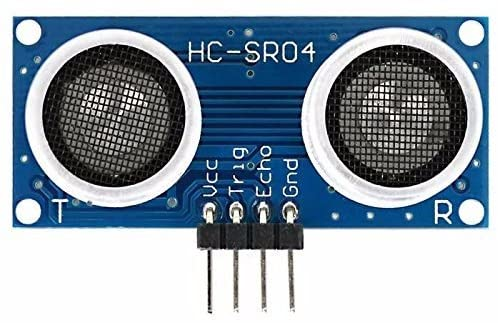
\includegraphics[width=.65\linewidth]{chapters/images/us.jpg} 
    \caption{Sensor ultrasonidos} 
  \end{minipage}%%
  \begin{minipage}[b]{0.5\linewidth}
    \centering
    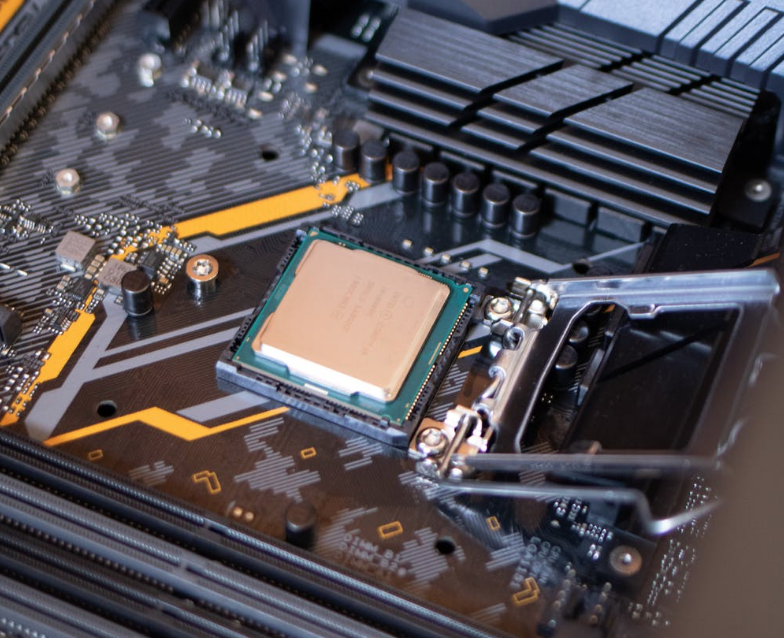
\includegraphics[width=.65\linewidth]{chapters/images/procesador.png} 
    \caption{Procesador} 
  \end{minipage} 
  \begin{minipage}[b]{0.5\linewidth}
    \centering
    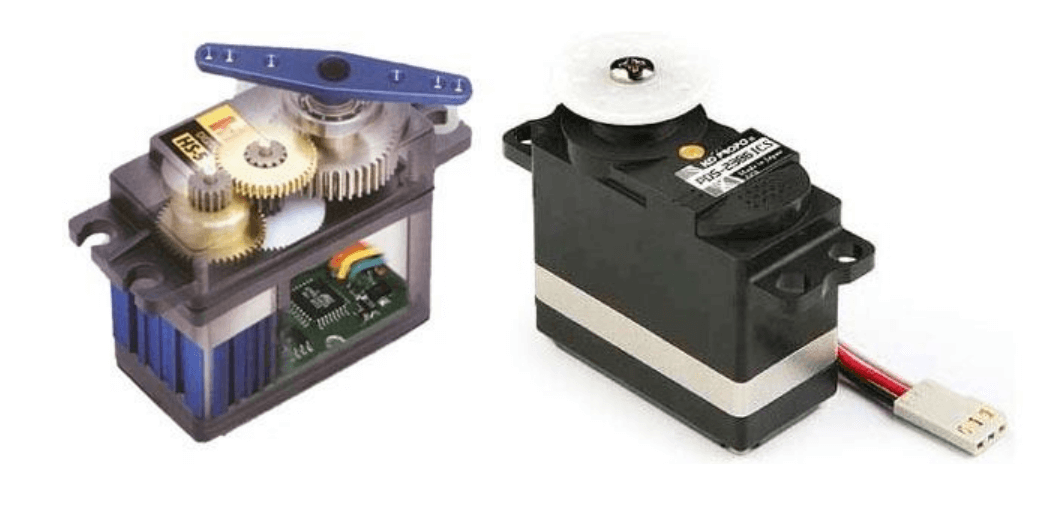
\includegraphics[width=.65\linewidth]{chapters/images/motor.png} 
    \caption{Servomotores} 
  \end{minipage}%% 
  \begin{minipage}[b]{0.5\linewidth}
    \centering
    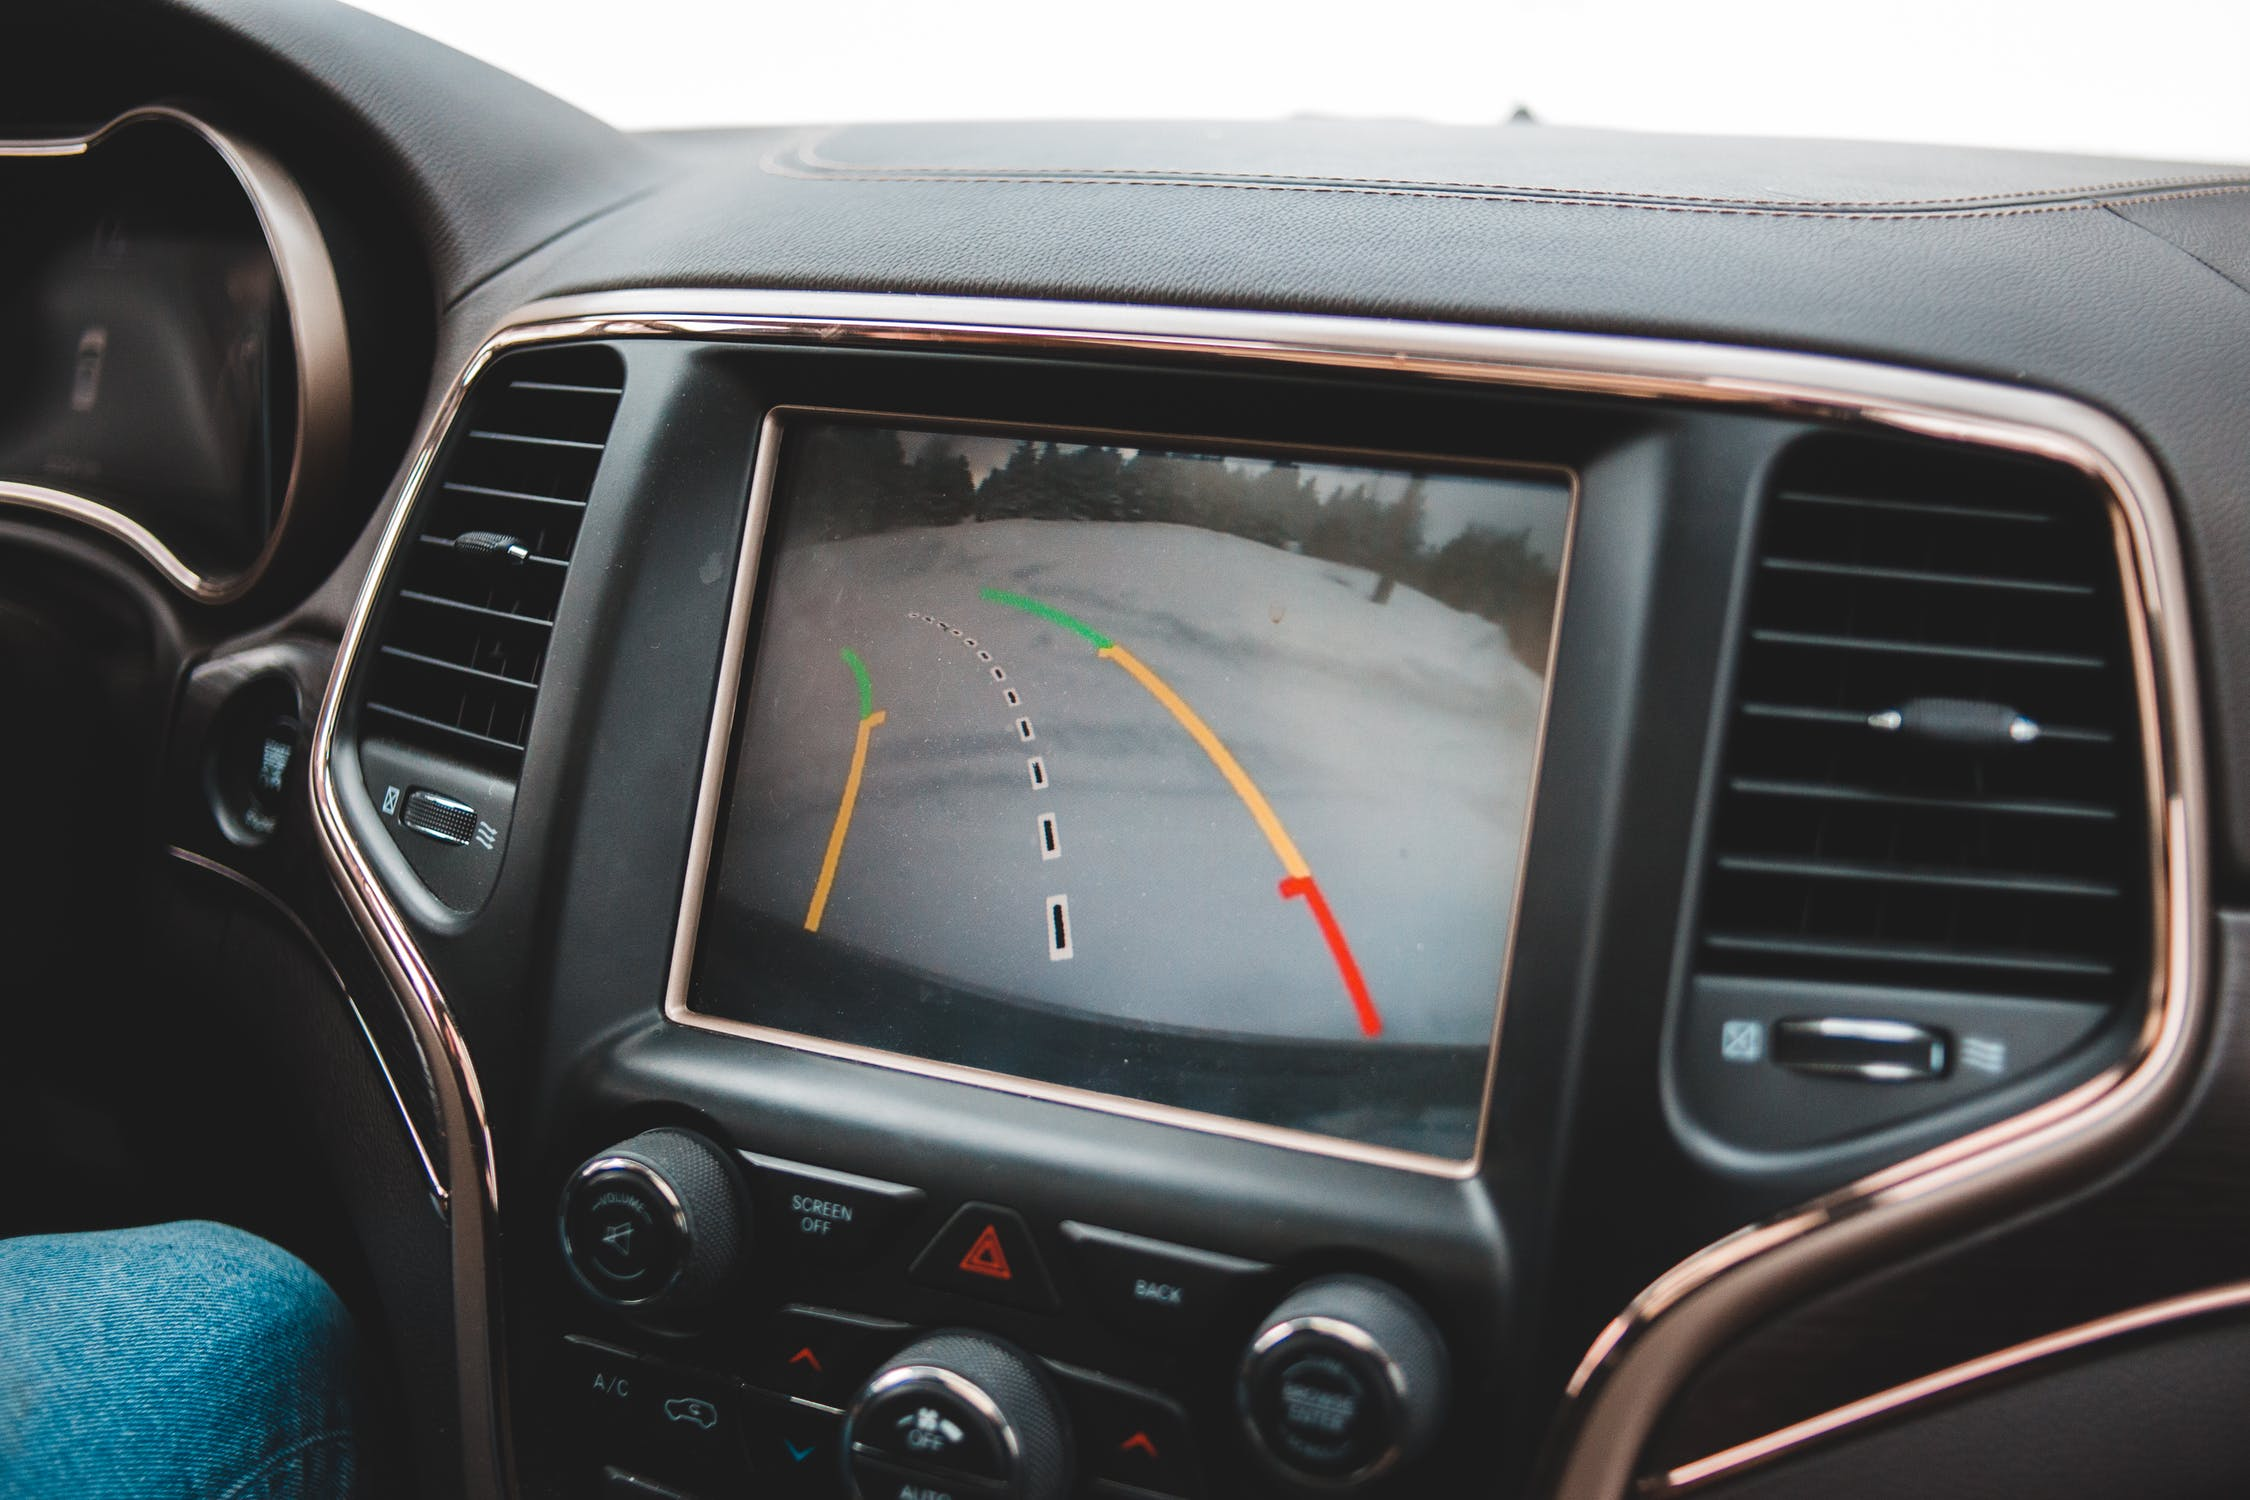
\includegraphics[width=.65\linewidth]{chapters/images/pantalla.jpeg} 
    \caption{Pantalla} 
  \end{minipage} 
\end{figure}

Los robots se clasifican según su entorno de aplicación en robots industriales y robots de servicio. También se pueden diferenciar según su forma en androides y zoomórficos, según su capacidad de movimiento en fijos o móviles, o según el medio en el que trabajan en terrestres, acuáticos o áereos. Estas son algunas de sus aplicaciones:
\begin{itemize}
    \item Robots industriales: brazos y pinzas robóticas para ensamblado de piezas, envasado de alimentos, industria automovilística y gestión de almacenes.
    \item Robots de servicio: destinados a limpieza del hogar, asistencia, coches autónomos, entrentenimiento, usos militares, limpieza de centrales nucleares, investigación en terrenos hostiles o fines médicos.
\end{itemize} 

 En la Figura 1.5 se muestran algunos ejemplos de robots que son de gran utilidad en la sociedad actual. 

\begin{figure}[H]
  \begin{subfigure}[b]{0.3\textwidth}
    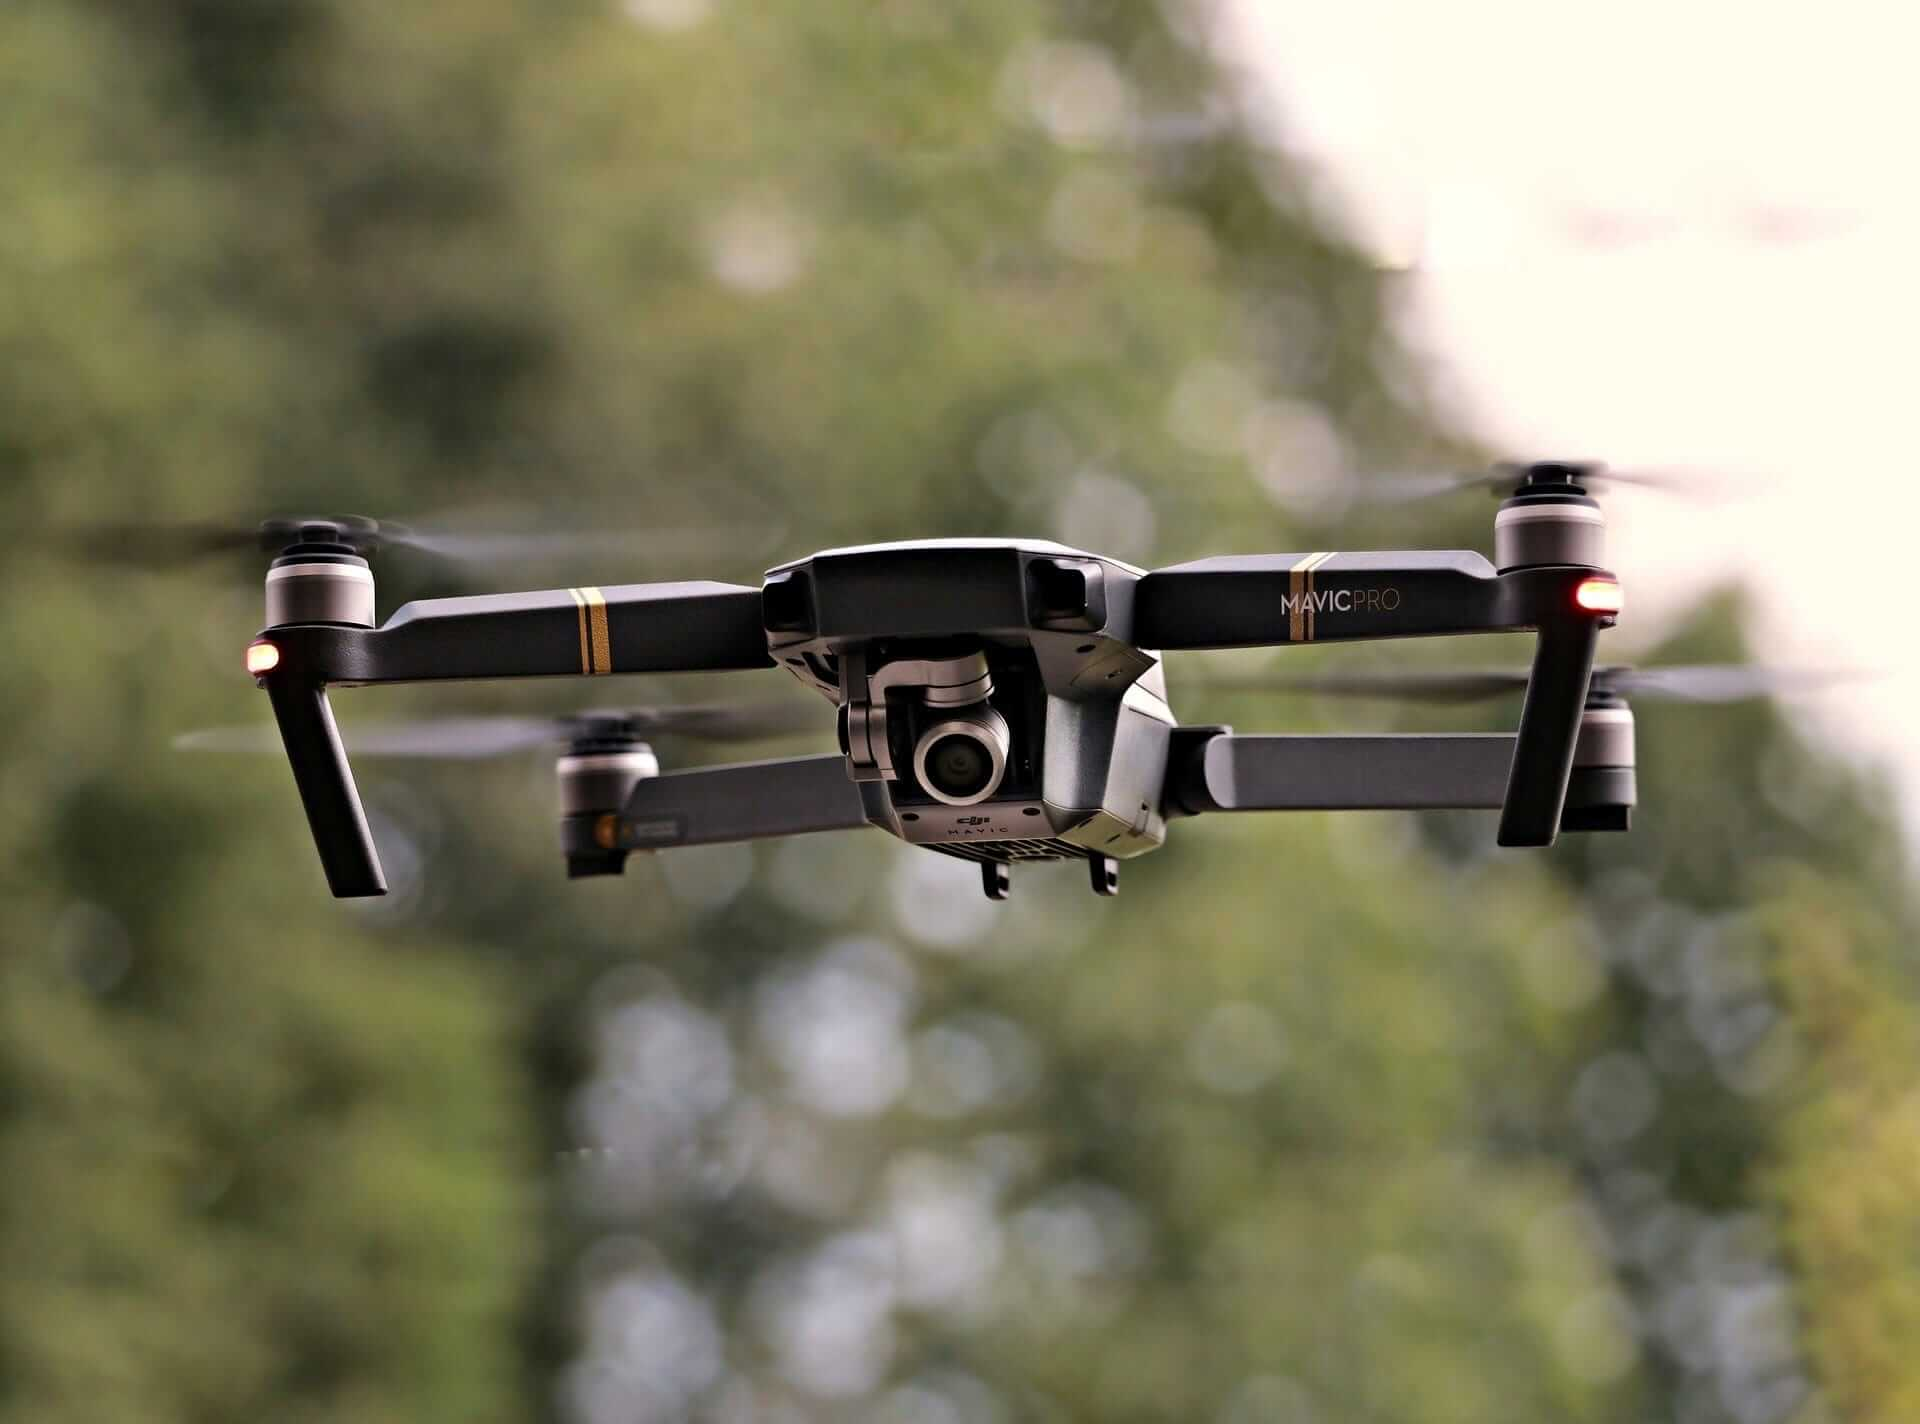
\includegraphics[width=\textwidth, height=\textwidth]{chapters/images/drone.jpeg}
    \caption{Dron}
    \label{fig:f1}
  \end{subfigure}
  \hfill
  \begin{subfigure}[b]{0.3\textwidth}
    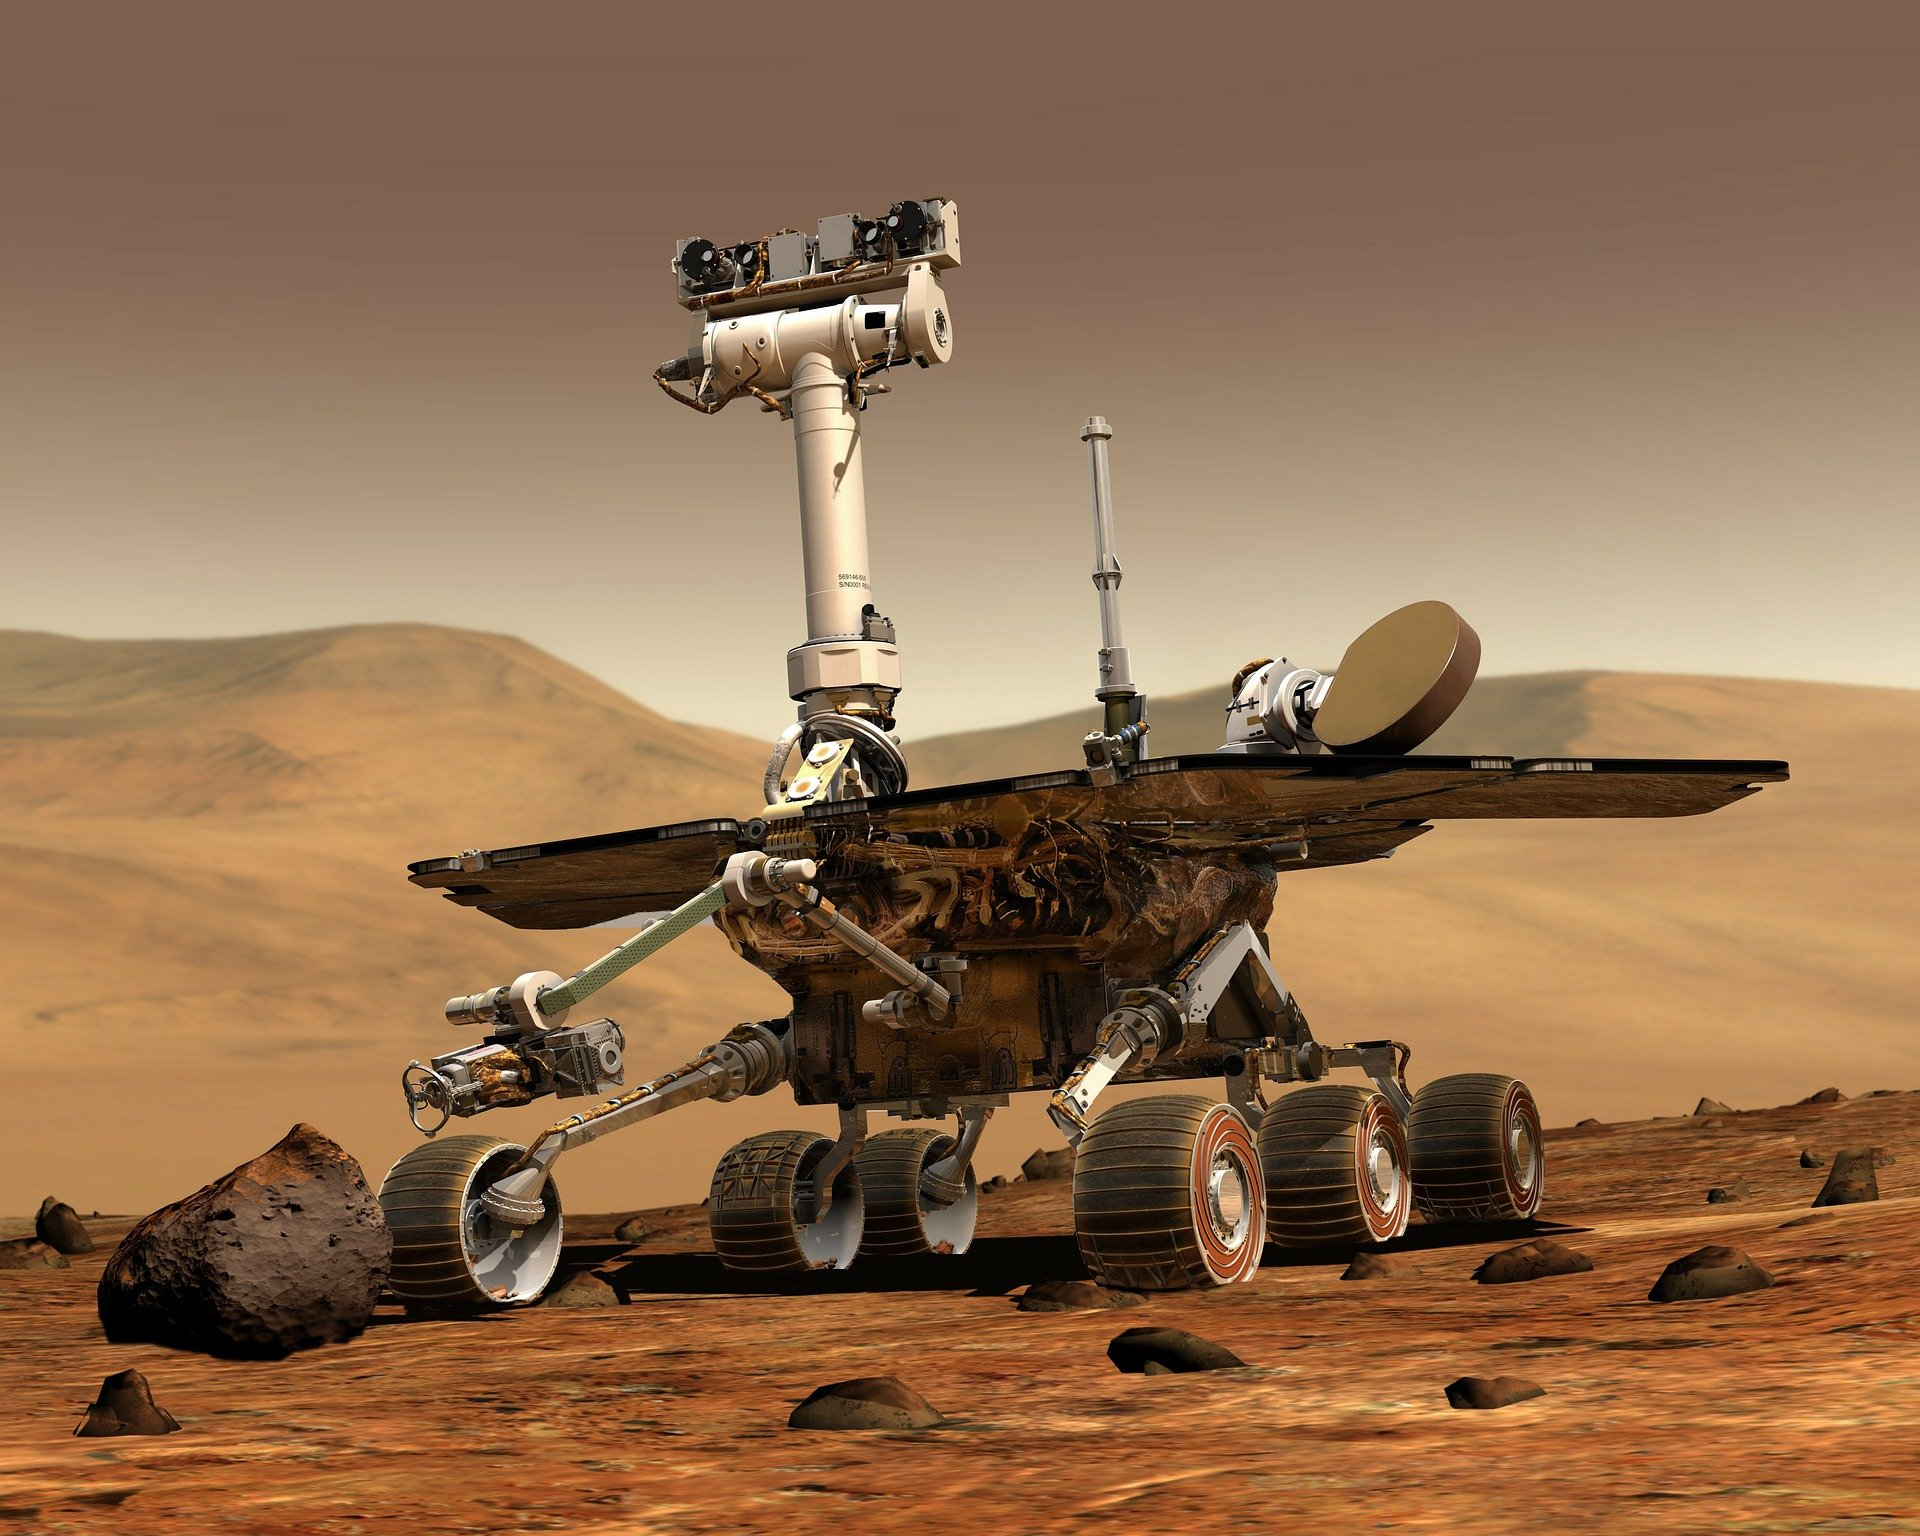
\includegraphics[width=\textwidth, height=\textwidth]{chapters/images/mars.jpg}
    \caption{Perseverance Mars}
    \label{fig:f2}
  \end{subfigure}
  \hfill
   \begin{subfigure}[b]{0.3\textwidth}
    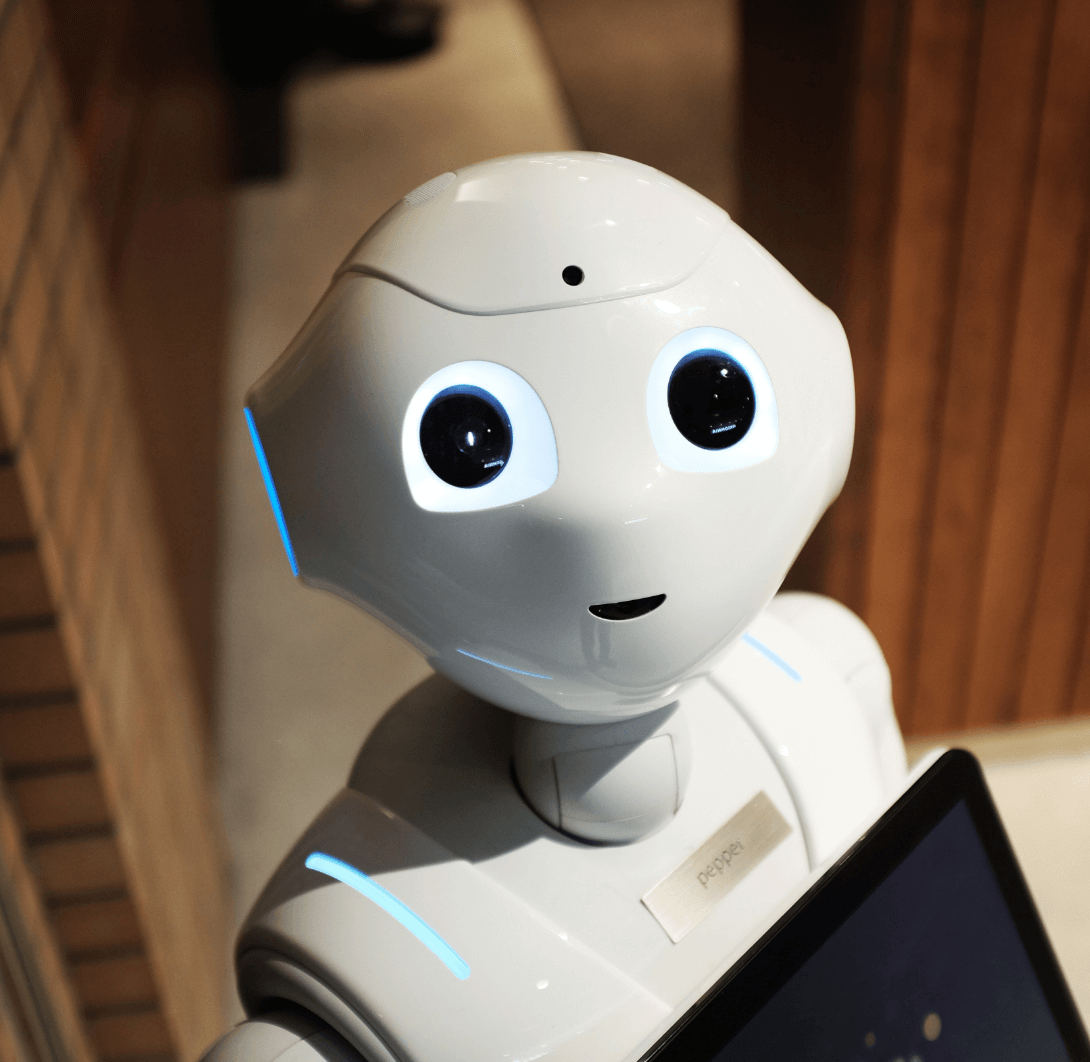
\includegraphics[width=\textwidth, height=\textwidth]{chapters/images/nao.png}
    \caption{Nao}
    \label{fig:f3}
  \end{subfigure}
  \hfill
   \begin{subfigure}[b]{0.3\textwidth}
    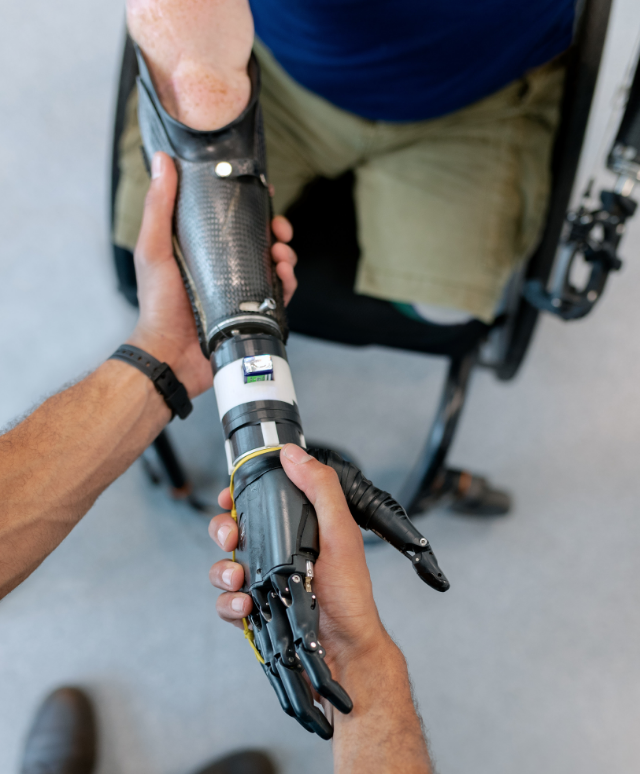
\includegraphics[width=\textwidth, height=\textwidth]{chapters/images/brazo.png}
    \caption{Brazo biónico}
    \label{fig:f4}
  \end{subfigure}
  \hfill
   \begin{subfigure}[b]{0.3\textwidth}
    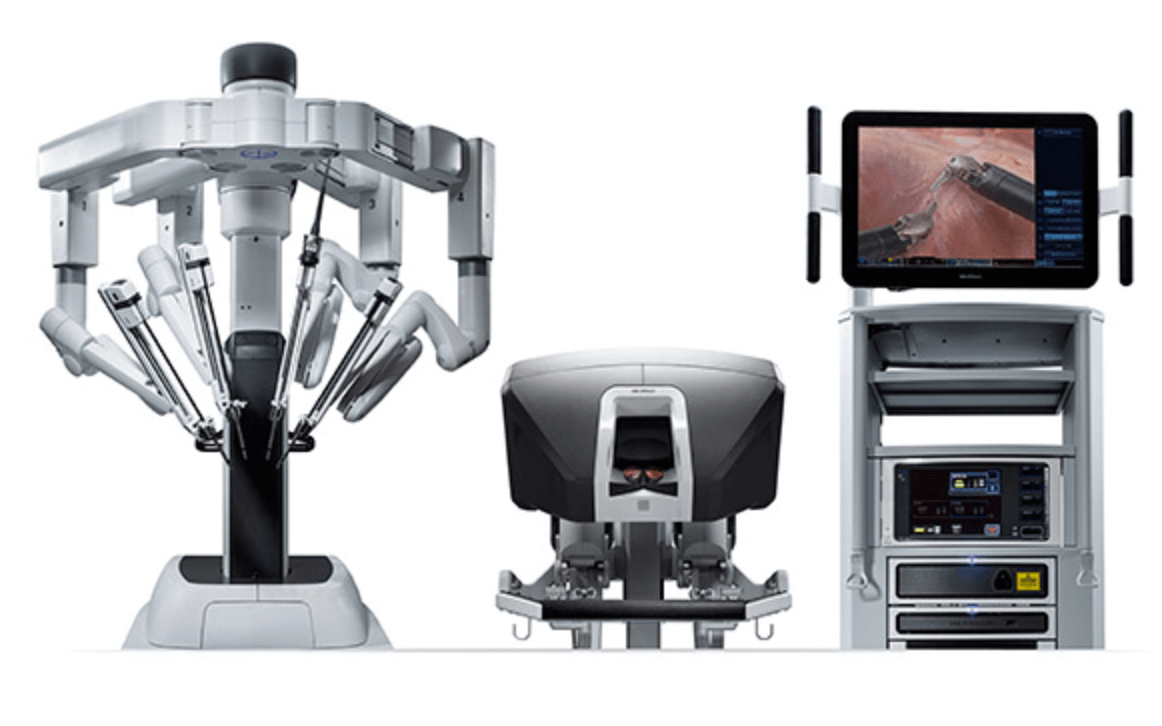
\includegraphics[width=\textwidth, height=\textwidth]{chapters/images/davinci.png}
    \caption{Da Vinci \cite{davinci} }
    \label{fig:f5}
  \end{subfigure}
  \hfill
   \begin{subfigure}[b]{0.3\textwidth}
    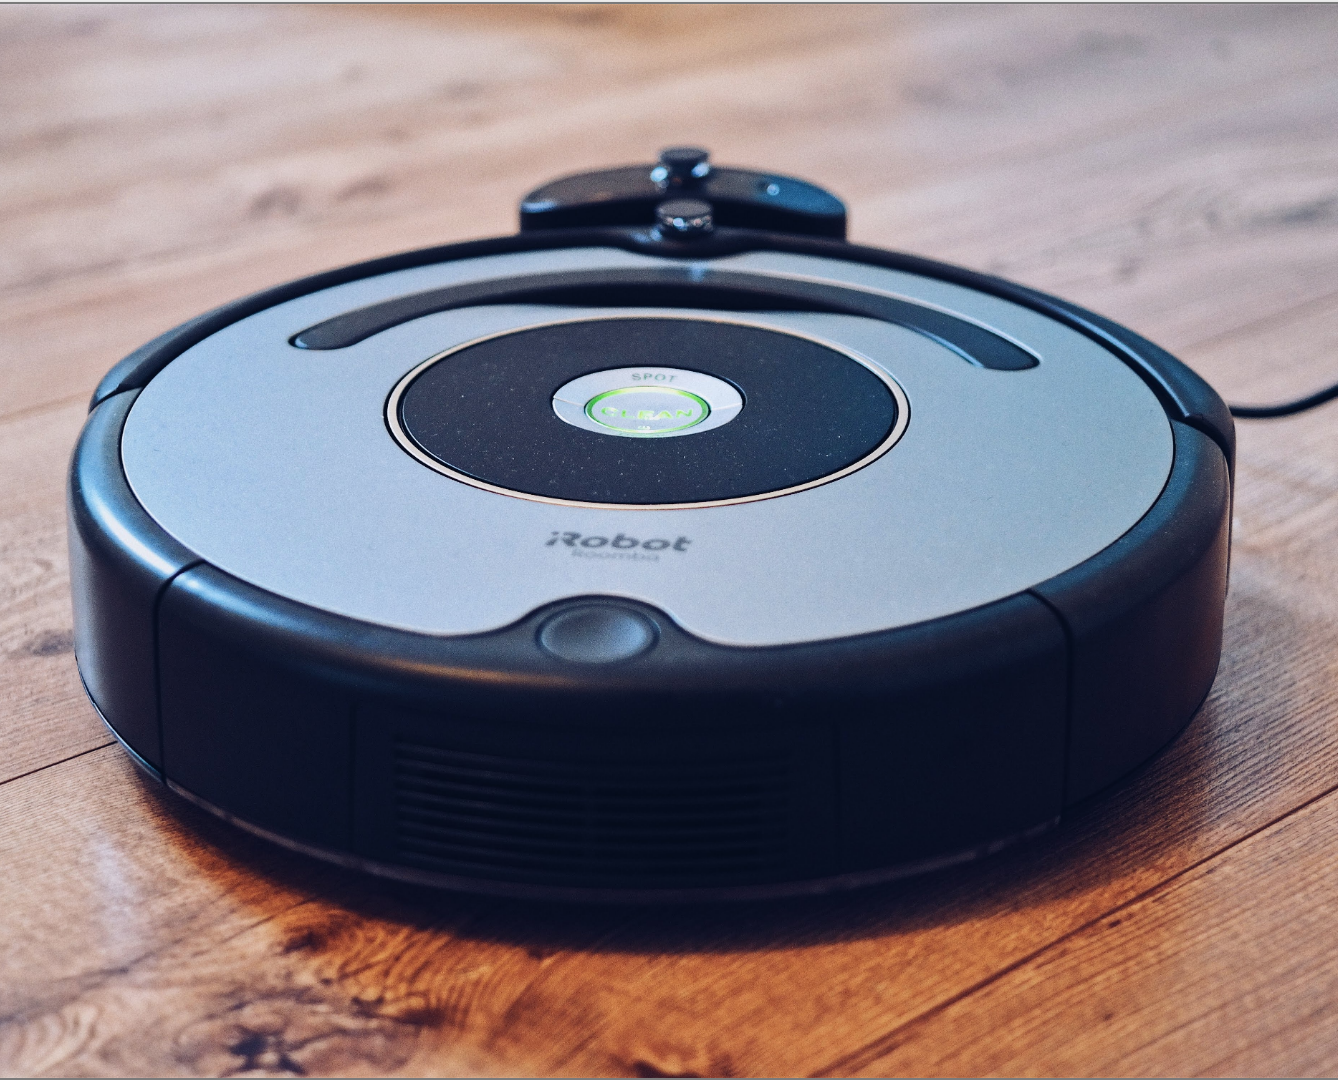
\includegraphics[width=\textwidth, height=\textwidth]{chapters/images/roomba.png}
    \caption{Roomba}
    \label{fig:f6}
  \end{subfigure}
  \caption{Ejemplos de Robots}
\end{figure}

La Figura 1.5(a) muestra un dron, estos pequeños vehículos no tripulados han sido toda una revolución en la grabación de eventos y películas. El entretenimiento no es su única aplicación, también se utilizan para la búsqueda de personas y vigilancia. 

El Perseverance Mars que vemos en la Figura 1.5(b) actualmente está en Marte haciendo investigaciones del terreno. Este robot busca signos de vida y guarda muestras para un futuro regreso a la Tierra.

Los robots de asistencia como el Nao, Figura 1.5 (c), son muy importantes para que los más pequeños y las personas mayores puedan socializar de una forma divertida y a su vez es una herramienta de apoyo en procesos de rehabilitación, post-operatorios y terapias ocupacionales.

Los brazos biónicos como el de la Figura 1.5(d) permiten recuperar las funciones y el tacto a amputados. El robot Da Vinci Figura 1.5(e) ayuda a los cirujanos a operar con mayor precisión y seguridad.  Estos robots han sido un gran avanze en el campo de la medicina.

El robot aspirador, uno del más conocido es \textit{Roomba}, Figura 1.5(f), es capaz de detectar obstáculos y residuos en el suelo. Esto nos ayuda a que la casa esté limpia y nos ahorra mucho tiempo.

Los robots que se han mencionado son solo algunos ejemplos. La robótica es una tecnología en auge. En los últimos años, con el avance de la tecnología, la realidad ha superado a la ficción, estamos rodeados de robots. Han salido de los laboratorios y han surgido miles de aplicaciones que nos hacen la vida un poco mejor.
\\
\\

Recientemente la robótica se está incorporando también a las aulas para que los más pequeños adquieran conocimientos y habilidades importantes para su futuro. En la siguiente Figura 1.6 se muestran unos ejemplos de robots diseñados para el ámbito educativo. \cite{roboticakids}

\begin{figure}[H]
    \centering
    \begin{subfigure}{.3\linewidth}
        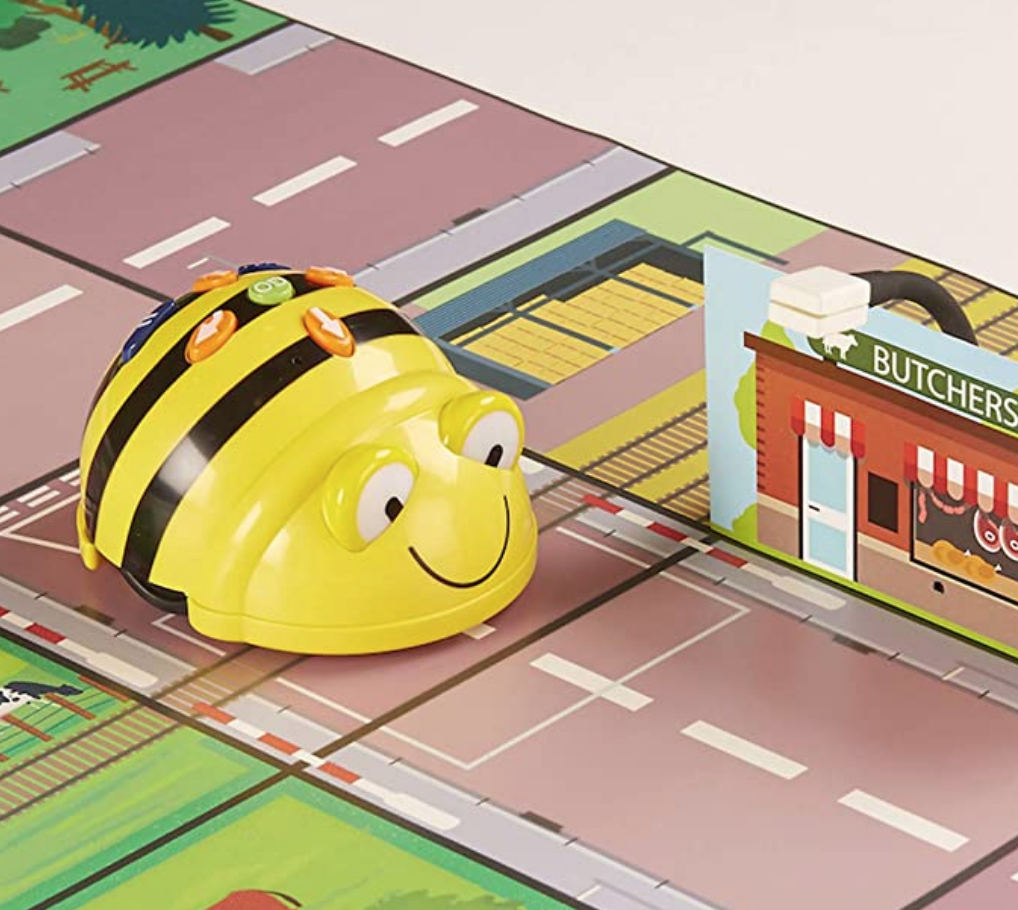
\includegraphics[width=1\textwidth]{chapters/images/beebot.png}
        \caption{Bee-bot}
    \end{subfigure}
    \hskip2em
    \begin{subfigure}{.3\linewidth}
    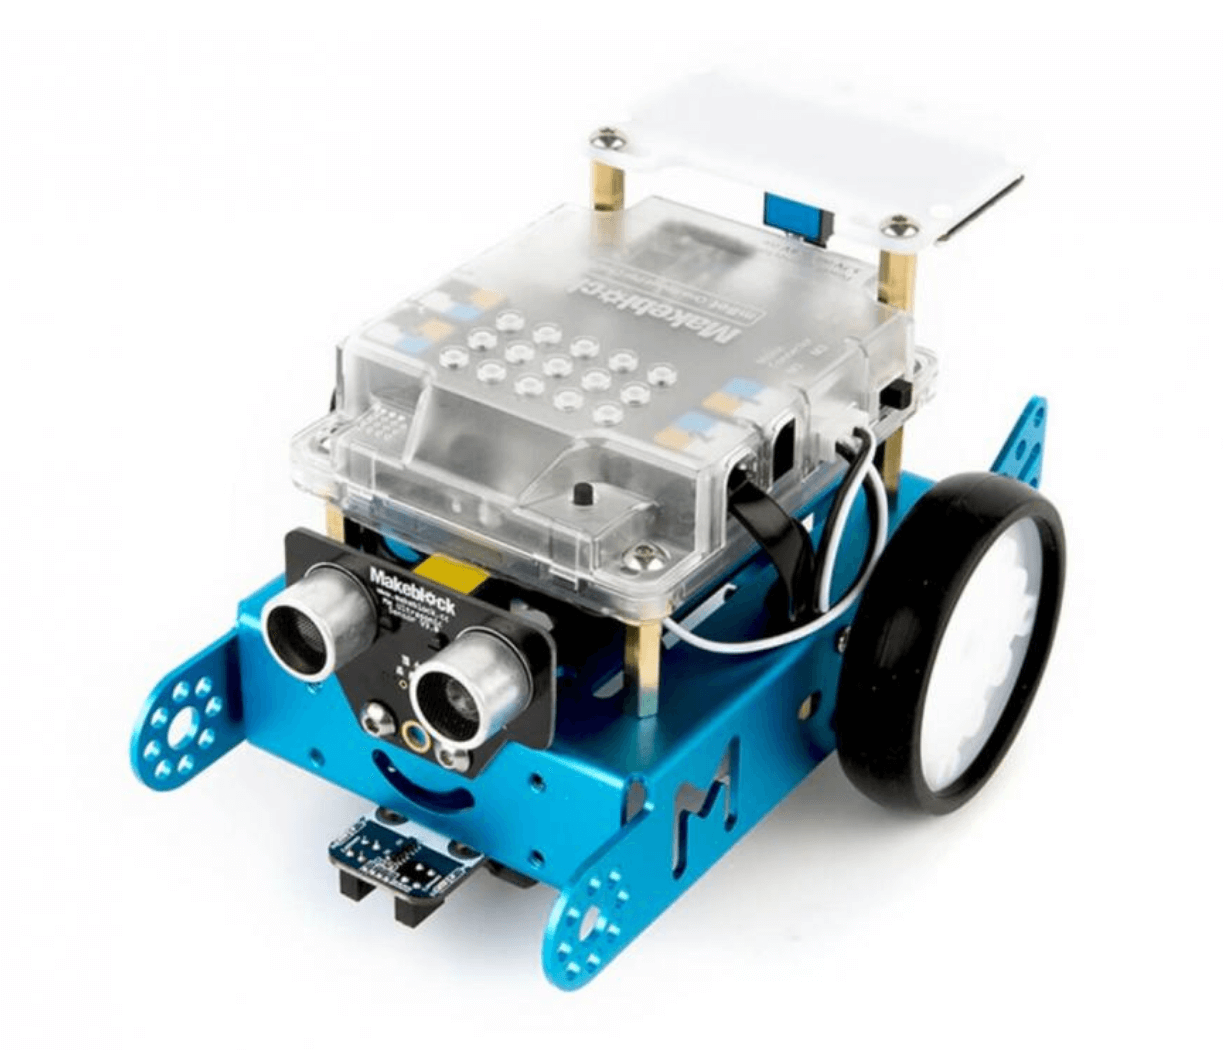
\includegraphics[width=1\textwidth]{chapters/images/mbot.png}
        \caption{Makeblock Mbot}
    \end{subfigure}
    \begin{subfigure}{.3\linewidth}
       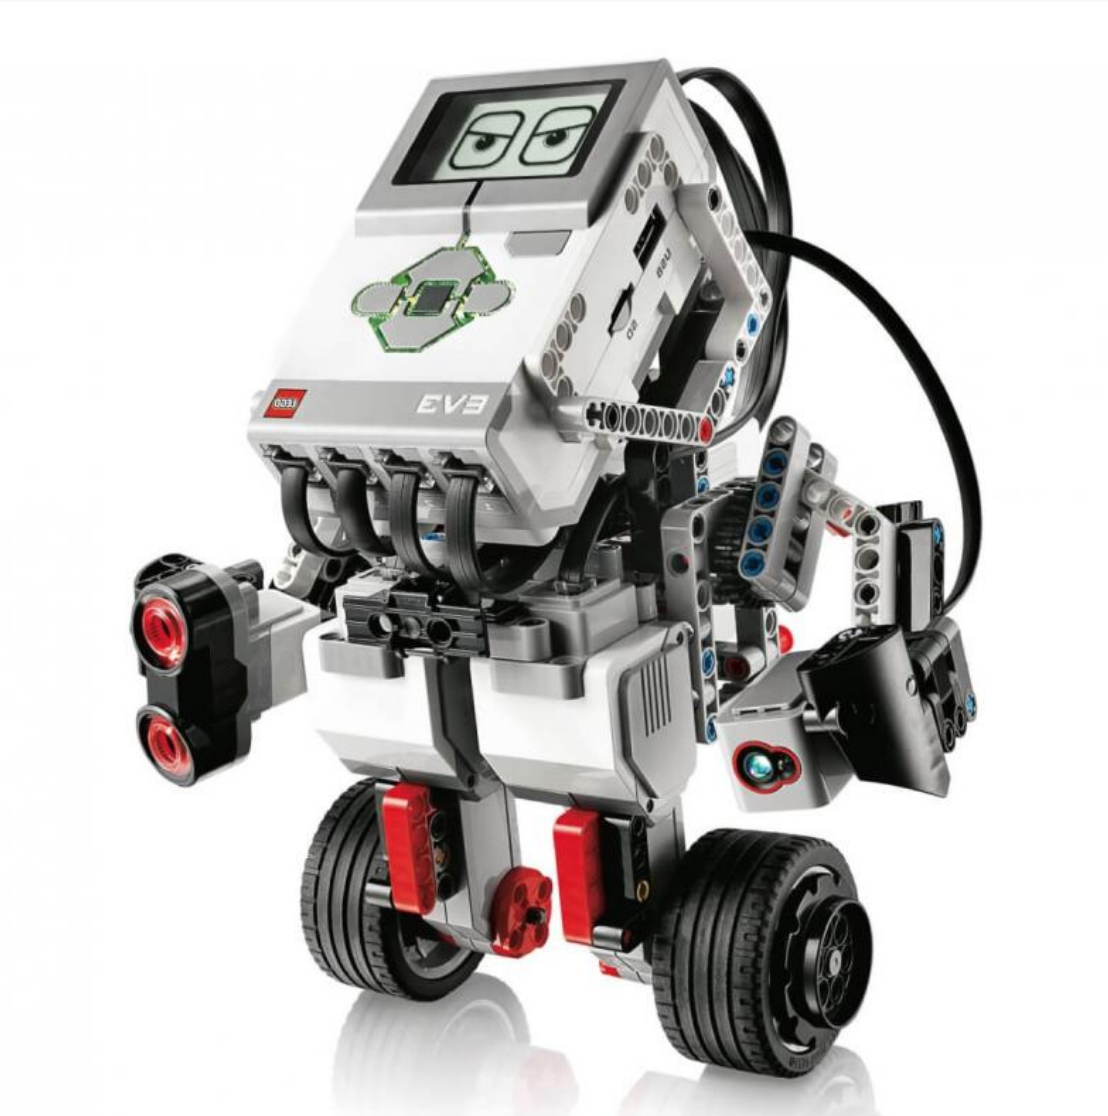
\includegraphics[width=1\textwidth]{chapters/images/lego.png}
        \caption{LEGO MINDSTORMS EV3}
    \end{subfigure}
    \caption{Ejemplos de Robots educativos}
\end{figure}


%%%%%%%%%%%%%%%%%%%%%%%%%
\newpage
\section{Tecnologías Web}
Las tecnologías web juegan un papel muy importante en el mundo moderno gracias a Internet. Esta plataforma WWW \footnote{World Wide Web}\cite{www}
ha ido evolucionando y ha posibilitado potentes aplicaciones con un modelo cliente/servidor. En la Figura 1.7 podemos ver algunos ejemplos de aplicaciones web.

\begin{figure}[H]
\begin{subfigure}{.5\textwidth}
  \centering
  % include first image
  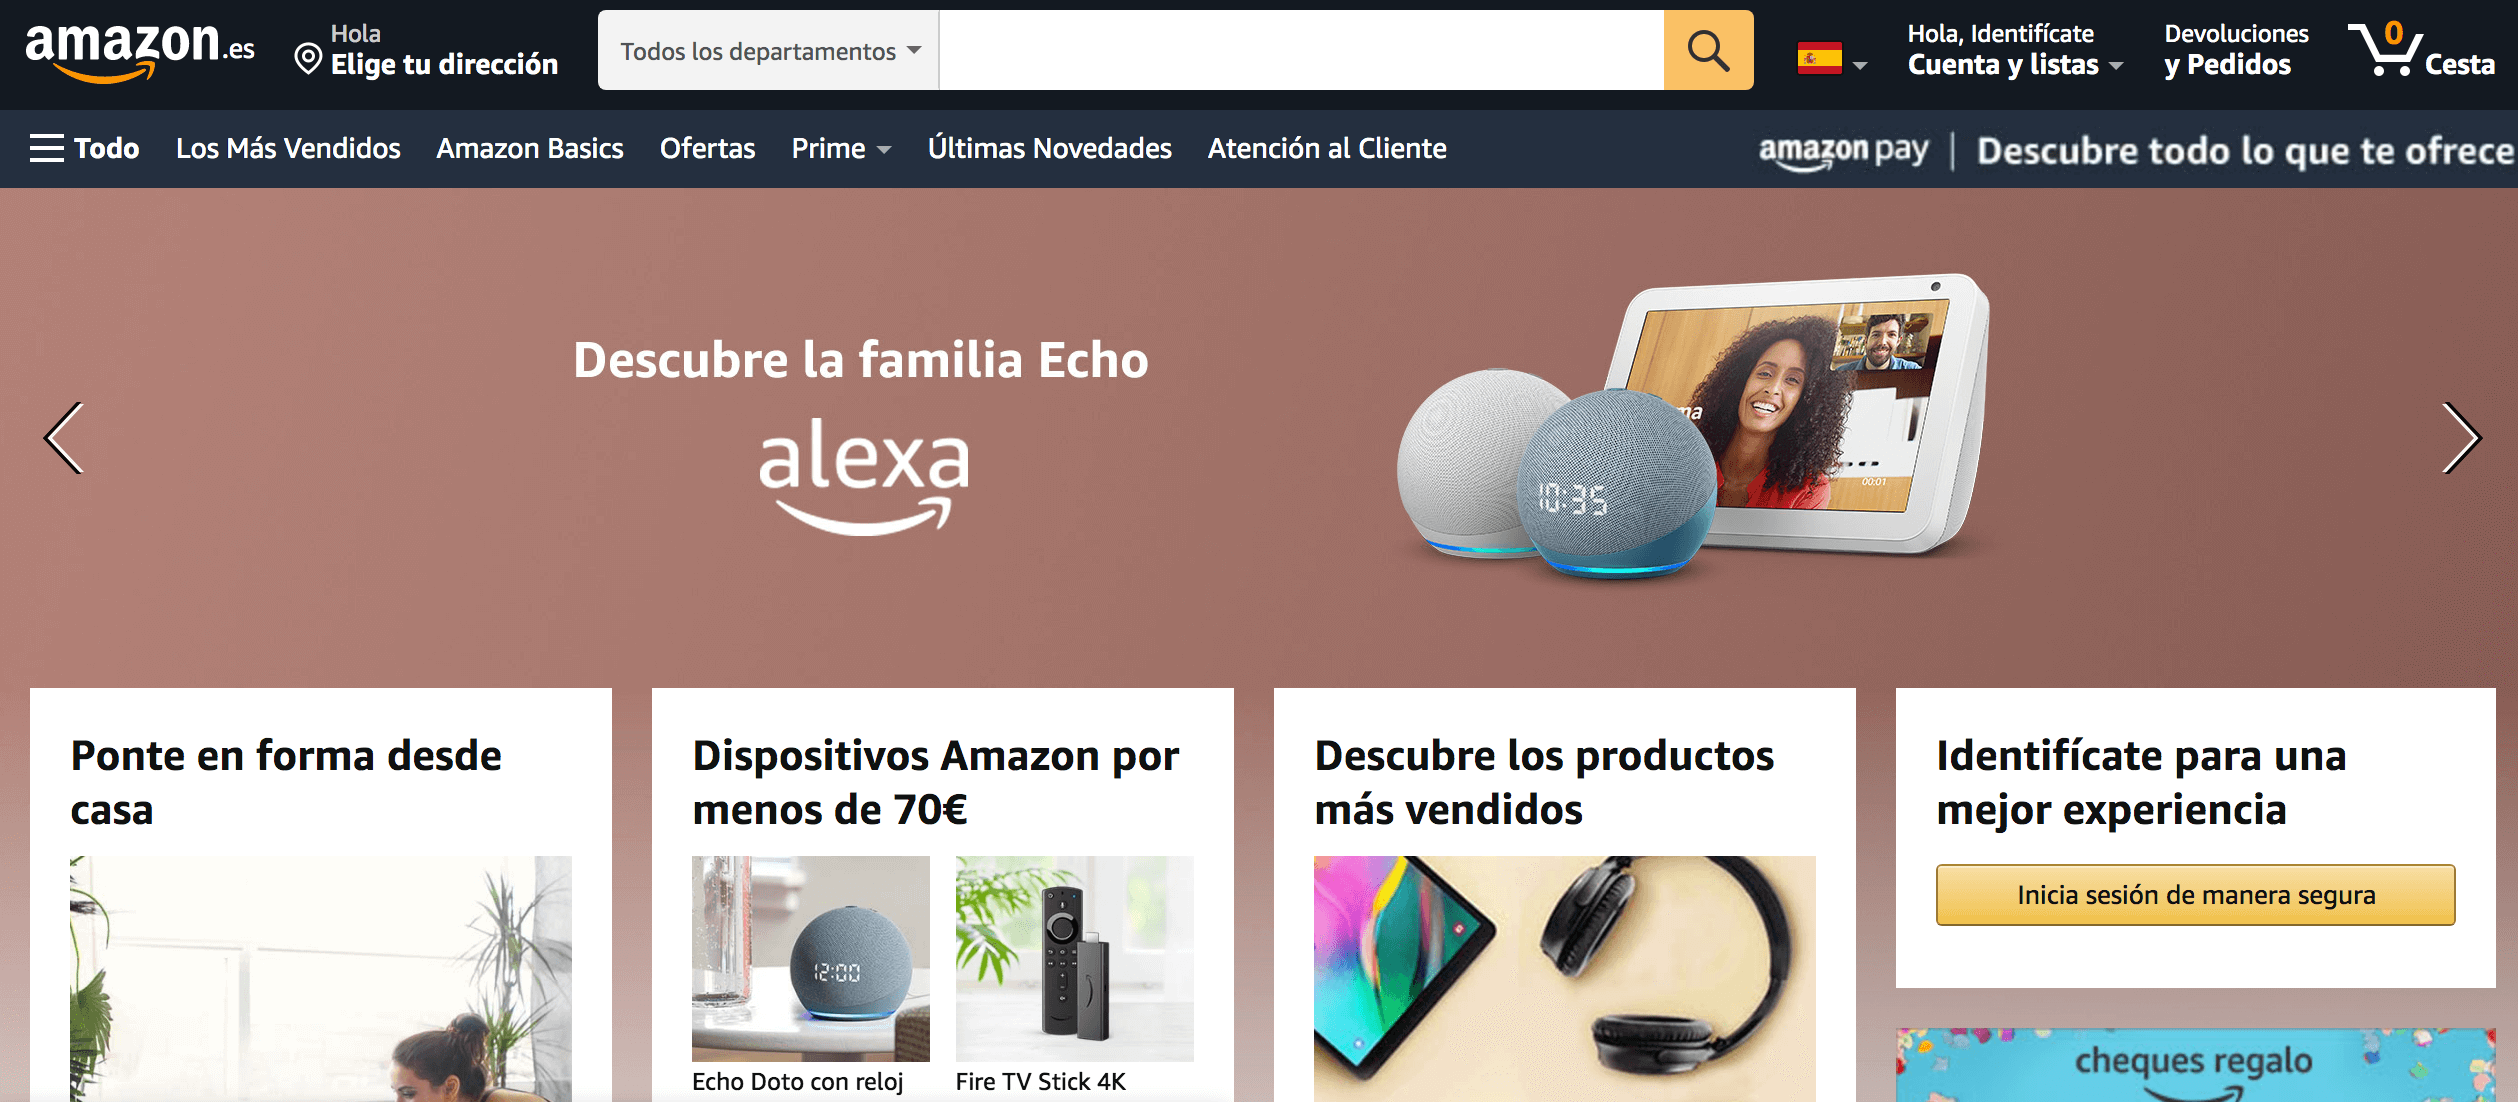
\includegraphics[width=.8\linewidth]{chapters/images/amazon.png}
  \caption{Amazon}
  \label{fig:sub-first}
\end{subfigure}
\begin{subfigure}{.5\textwidth}
  \centering
  % include second image
  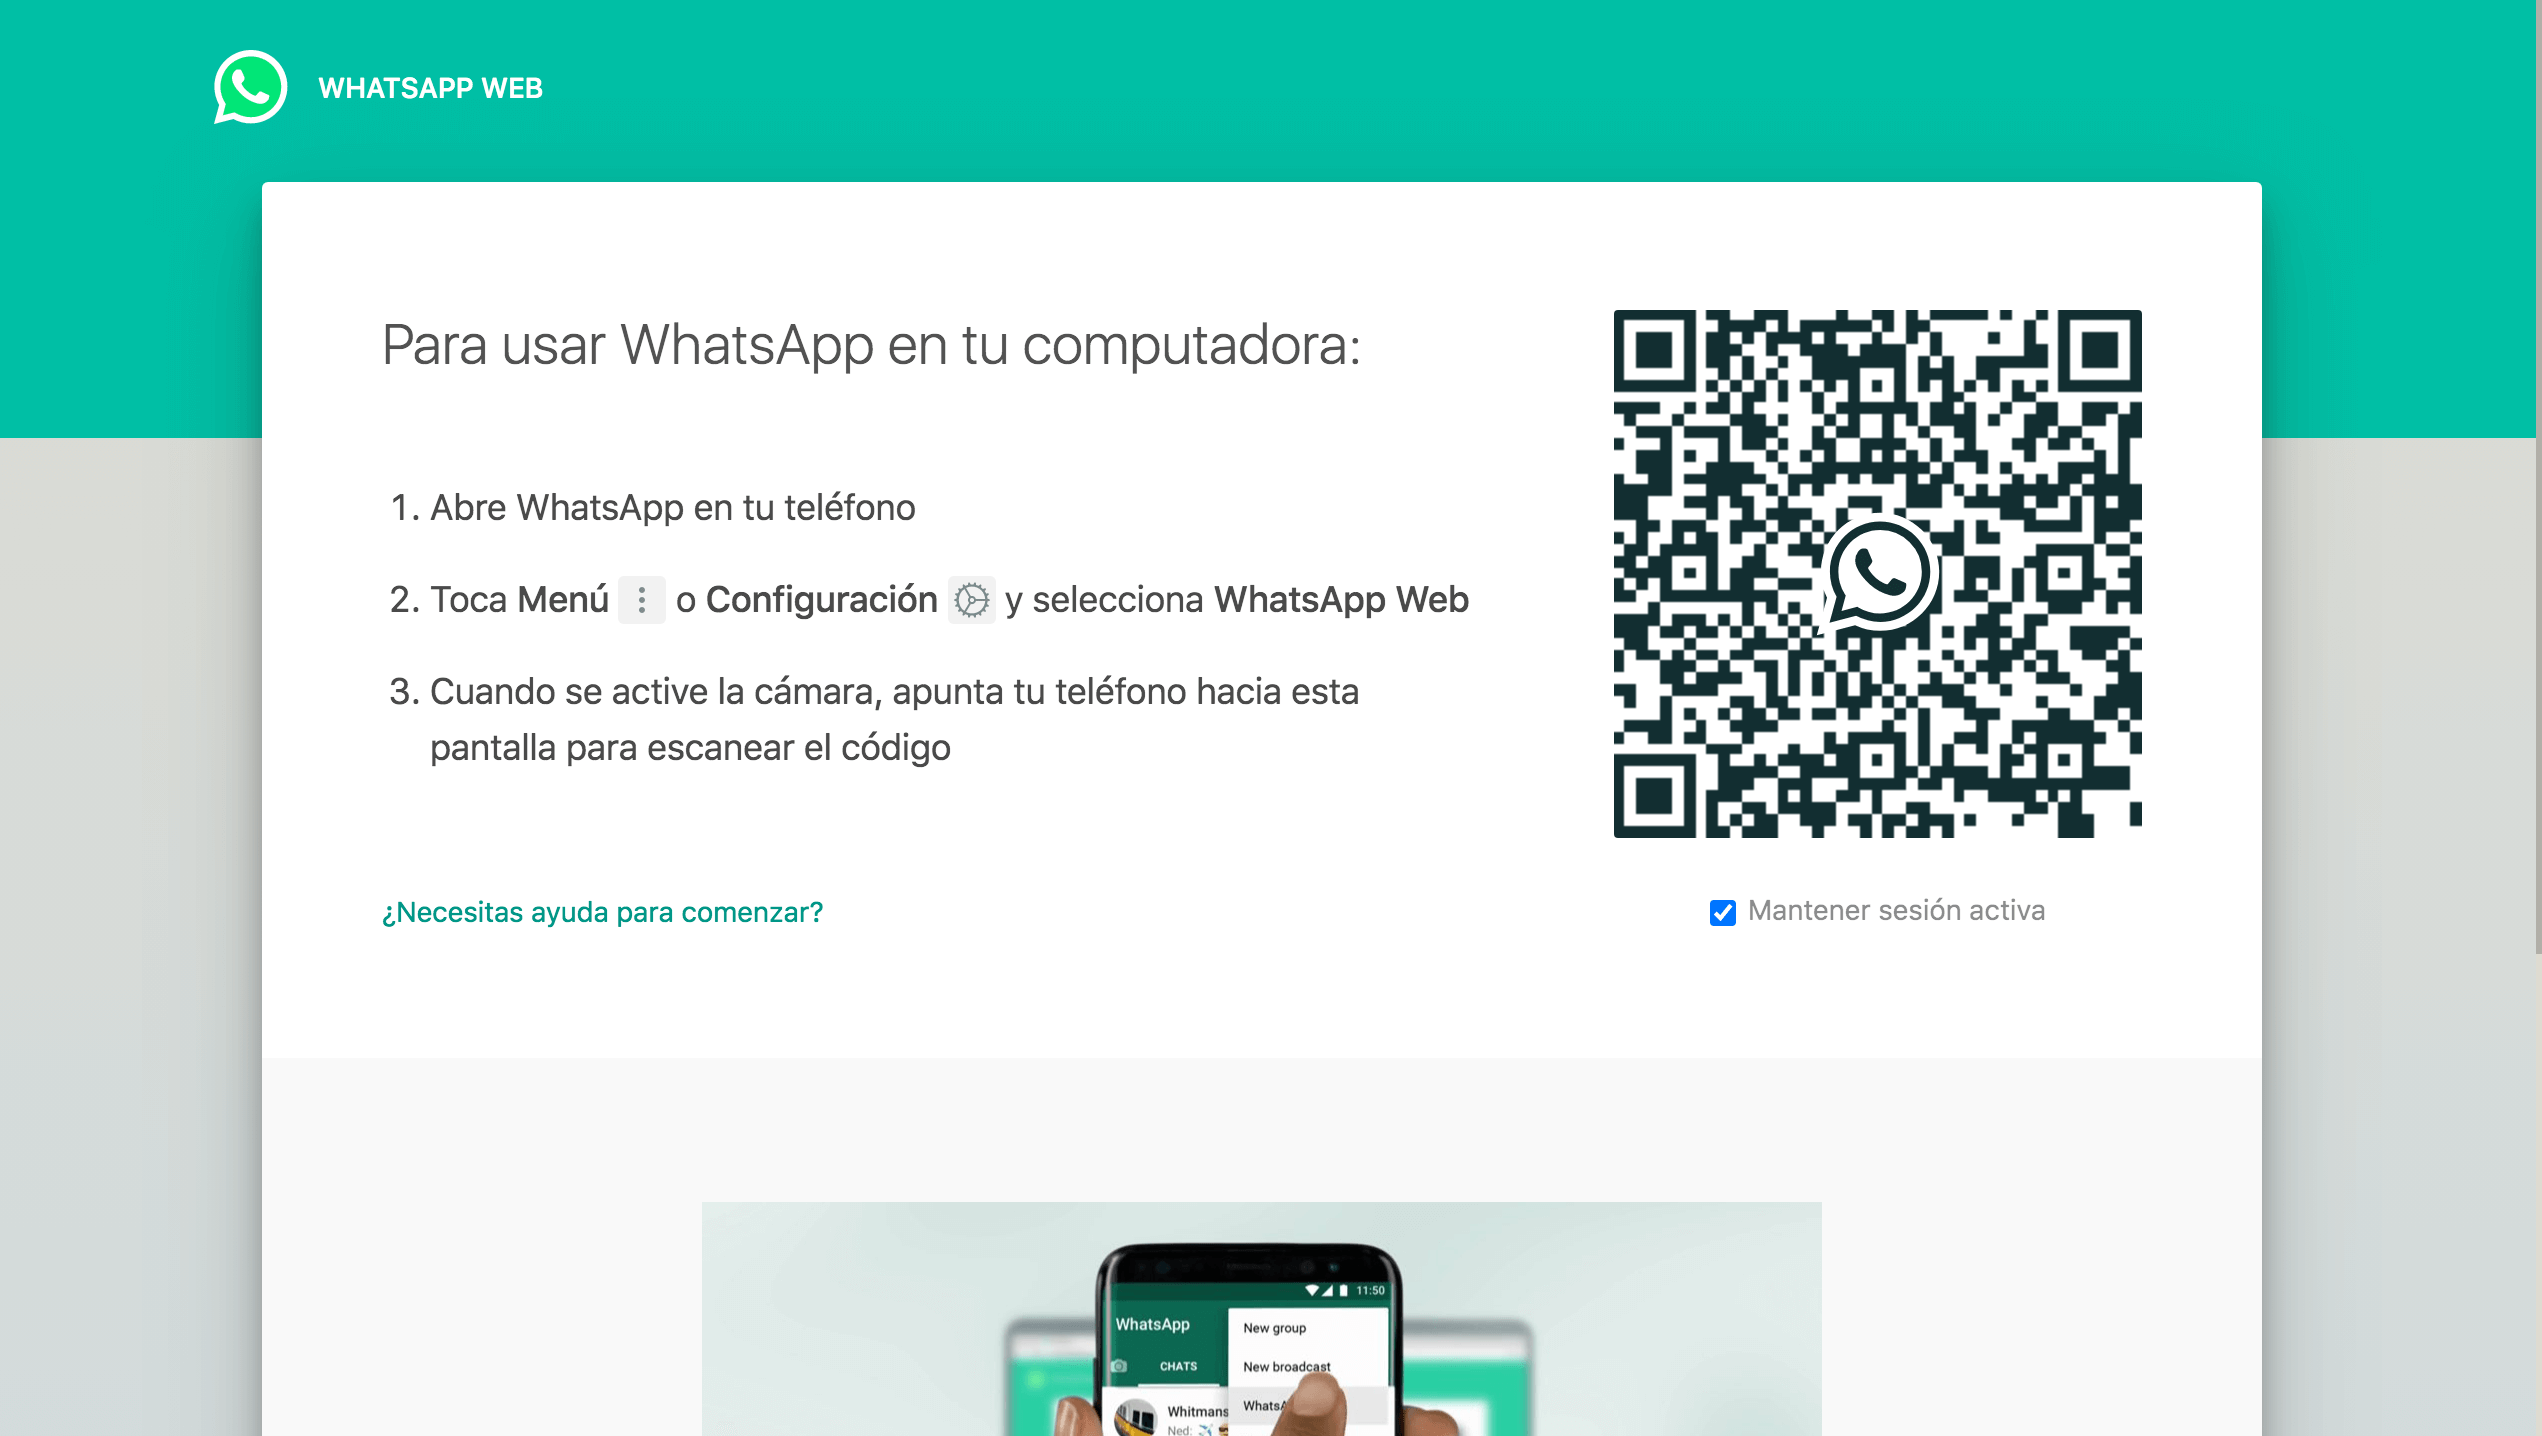
\includegraphics[width=.8\linewidth]{chapters/images/whatsappweb.png}  
  \caption{Whatsapp Web}
  \label{fig:sub-second}
\end{subfigure}
\begin{subfigure}{.5\textwidth}
  \centering
  % include third image
  
\includegraphics[width=.8\linewidth]{chapters/images/disney.jpeg}  
  \caption{Disney+}
  \label{fig:sub-third}
\end{subfigure}
\begin{subfigure}{.5\textwidth}
  \centering
  % include fourth image
  
\includegraphics[width=.8\linewidth]{chapters/images/urjcweb.png}  
  \caption{URJC}
  \label{fig:sub-fourth}
\end{subfigure}
\caption{Ejemplos aplicaciones web}
\label{fig:partes robot}
\end{figure}

La web es una colección de documentos enlazados a través de hiperenlaces, cada recurso queda definido por su URL \footnote{Uniform Resource Locator}. Cuando accedemos a la web a través del navegador, tenemos que introducir la dirección URL del sitio web al que nos queremos dirigir. El navegador enviará una solicitud al servidor con el protocolo HTTP \footnote{Hyper Text Transfer Protocol}. El servidor le enviará a nuestro navegador un fichero HTML que quedará almacenado en nuestra máquina. Una vez el navegador obtiene el fichero HTML mostrará al usuario la página web principal de la URL que ha introducido. Si el navegador detecta que hay imágenes, vídeos u otros ficheros, volverá a mandar peticiones HTTP al servidor para que éste le envíe toda la información necesaria. En la Figura 1.8 podemos ver una representación de cómo es la comunicación entre cliente y servidor.
\begin{figure}[H]
    \centering
    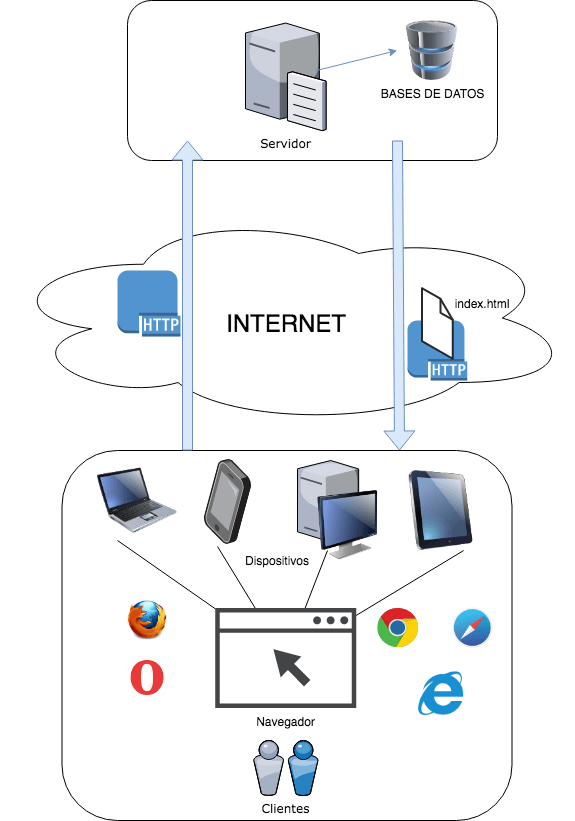
\includegraphics[width=0.45\columnwidth]{chapters/images/web.png}
    \caption{Comunicación cliente/servidor a través de HTTP}
    \label{fig:httpprotocol}
\end{figure}
 HTTP es un protocolo entre navegadores y servidores web para transferir documentos de hipertexto. El cliente envía mensajes de solicitud y el servidor manda mensajes de respuesta, ambos mensajes son del mismo formato (ver Figura 1.9 y Figura 1.10.) Los tipos de mensaje más comunes de este protocolo son GET, POST, PUT, DELETE y HEAD. Este protocolo utiliza códigos de estado, los más conocidos son: 200 OK, que significa resultado exitoso, 500 Server Error, cuando hay un error en el lado servidor y el más conocido 404 Not Found, cuando hay un error en la parte cliente. \cite{tecnologiasweb}

\begin{figure}[H]
\centering
\begin{minipage}[t]{.45\linewidth}
\centering
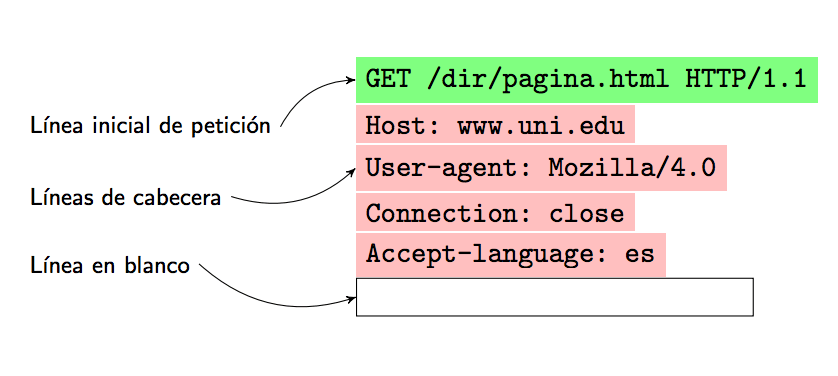
\includegraphics[width=1\columnwidth]{chapters/images/peticionhttp.png}
\caption{Ejemplo petición HTTP\\ Cliente a Servidor}
\end{minipage}
\hspace{0.25in}
\begin{minipage}[t]{.45\linewidth}
\centering
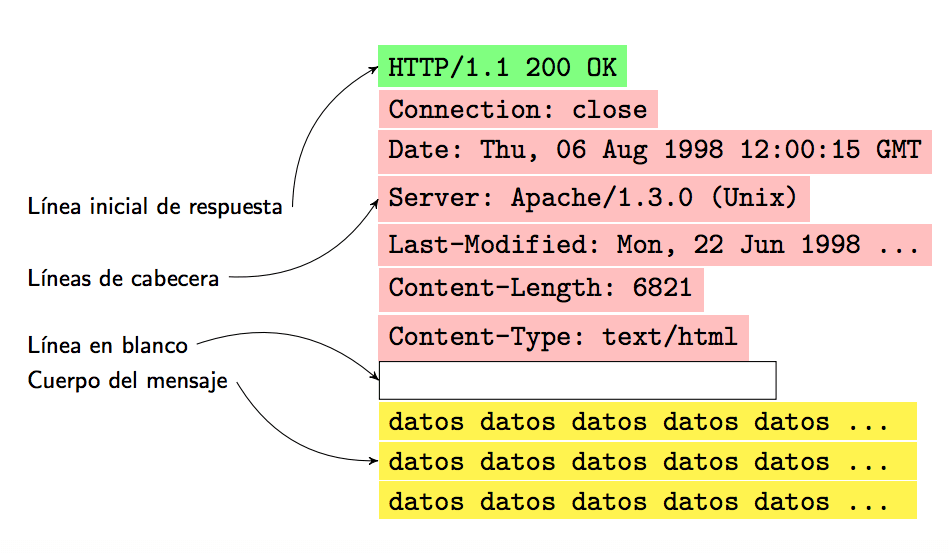
\includegraphics[width=1\columnwidth]{chapters/images/respuestahttp.png}
\caption{Ejemplo respuesta HTTP\\ Servidor a Cliente}
\end{minipage}
\end{figure}


Las dos partes que forman una aplicación web son independientes entre sí. Las tecnologías del  lado cliente (\textit{frontend}) se encargan de  interactuar con el usuario, visualizar el contenido y establecer la comunicación con el servidor. Se ejecutan en el navegador, que actúa como intérprete. Por otro lado, las tecnologías del lado servidor (\textit{backend}) se encargan de la administración del sitio web, usando bases de datos y gestores de contenidos.

Una de las principales ventajas de usar tecnologías web es que las aplicaciones creadas son multiplataforma y multidispositivo, funcionan tanto en ordenadores, móviles, tabletas, así como en distintos sistemas operativos. Otra ventaja es que no tenemos que instalar nada, sólo necesitamos el navegador y además la actualización del contenido es inmediata. El principal inconveniente es su dependencia de Internet, pero con los últimos avances tecnológicos el Wifi, la fibra óptica y el 5G han permitido que  mayoría de personas del mundo podamos acceder desde cualquier lugar y éste no sea un gran inconveniente.


\subsection{Tecnologías Web lado cliente}
Las tecnologías web del lado cliente  permiten la interacción del usuario con la página web que corre en el navegador del usuario. Para ello, se usan principalmente estas tres tecnologías \cite{tecnologiascliente}:

\begin{itemize}
  \item HTML5 \footnote{HyperText Markup Language}: es un lenguaje de marcado de los contenidos de un sitio web, se usa para asignar la función de cada elemento. Es el esqueleto de la web.
  \item JavaScript: es un lenguaje de programación interpretado que se encarga del comportamiento de una página web y de su interactividad con el usuario.
  \item CSS3\footnote{Cascading Style Sheets}: es un lenguaje de hojas de estilo creado para controlar la presentacion de la página: colores, tipo de letra, tamaños, animaciones, colocación de los elementos...
\end{itemize}

Entraremos en más detalle en estas tecnologías en el capítulo 3 donde se habla de la Infraestructura utilizada.

\newpage
\subsection{Tecnologías Web lado servidor}
Las tecnologías web del lado servidor son las que permiten gestionar y servir las páginas web y acceder a bases de datos. En este caso las tecnologías son más flexibles y vamos a nombrar tres de las más utilizadas:

\begin{itemize}
    \item Django: es un entorno para crear servidores web de alto nivel, que fomenta el desarrollo rápido con un diseño limpio y práctico en Python, destaca por su arquitectura basada en  modelo-vista-controlador y el uso de plantillas. De esta forma puedes centrarte en crear tu aplicacion web sin grandes complicaciones. Es gratis y de código abierto\cite{django}. Un ejemplo de aplicación web que utiliza Django es Instagram \cite{insta}.
    \item Node.js: es un entorno de ejecución para JavaScript orientado a eventos síncronos, construido con el motor de JavaScript V8 de Chrome. Diseñado para aplicaciones web escalables. De esta forma el cliente y el sevidor pueden crearse con el mismo lenguaje de programación\cite{node}. Netflix, Paypal o LinkedIn usan esta tecnología para sus servidores\cite{nodenetflix}. 
    
    \item PHP\footnote{Hypertext Preprocessor}: es un lenguaje de scripting de uso general popular que es especialmente adecuado para el desarrollo web\cite{php1}. Rápido, flexible y práctico, gracias a su capacidad de creación de webs dinámicas, desde blogs hasta sitios web como Facebook o Wikipedia\cite{php2}.
    
\end{itemize}

En el lado servidor se utilizan bases de datos. Una base de datos es una colección de datos estructurados. Entre ellas podemos destacar mySQL(Figura 1.11a) y MongoDB(Figura 1.11 b). 

\begin{figure}[H]
  \begin{subfigure}[b]{0.5\textwidth}
  \centering
    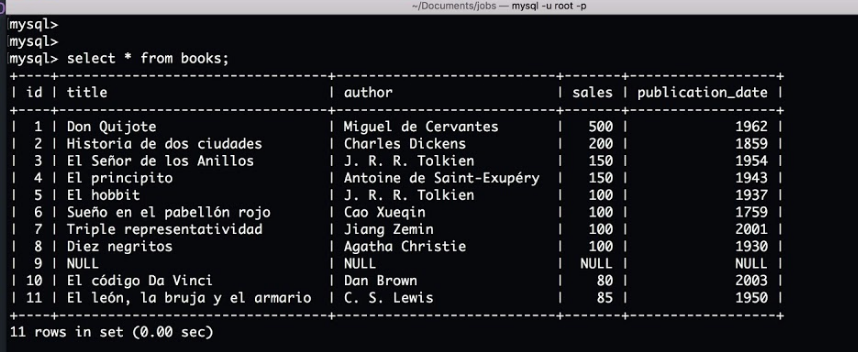
\includegraphics[width=1\textwidth, height=0.7\textwidth]{chapters/images/mysql.png}
    \caption{mySQL}
    \label{fig:f1}
  \end{subfigure}
  \hfill
  \begin{subfigure}[b]{0.5\textwidth}
  \centering
    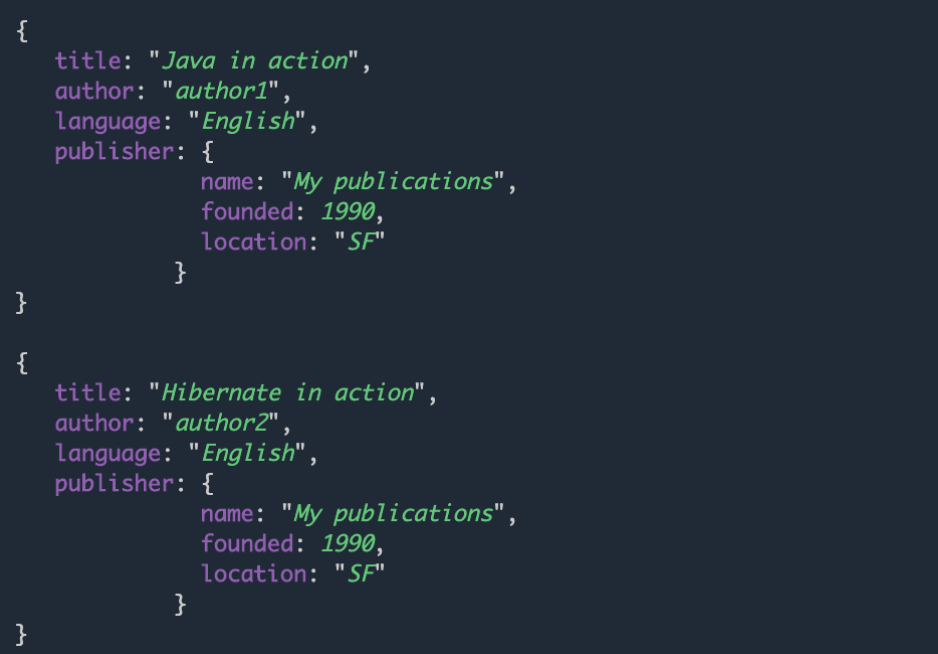
\includegraphics[width=1\textwidth, height=0.7\textwidth]{chapters/images/mongodb.png}
    \caption{MongoDB}
    \label{fig:f2}
  \end{subfigure}
  \caption{Bases de Datos}
\end{figure}



%%%%%%%%%%%%%%%%%%%%%%%%%%%%%%%%%%%%%%%%%%%%%%%%%%%%%%%%%%%%%%%%%%%%%%%%%%%%%%%%%%%%%%%%%%%%%%%%%%%%%%%%%%%%%%%%
\newpage
\section{Robótica educativa}

La Robótica educativa es un sector de aprendizaje multidisciplinar. Ayuda a desarrollar competencias y habilidades como: la innovación y espíritu emprendedor, la resolución de problemas y lógica, la toma de decisiones, conocimientos de herramientas relacionadas con las tecnologías digitales, el pensamiento crítico, creatividad, el trabajo colaborativo y cooperativo, la flexibilidad y adaptabilidad al trabajo \cite{roboticaedu}.
\\
Ante la falta de estudiantes en carreras técnicas en la actualidad, la robótica educativa puede ofrecer una gran motivación a los alumnos de las primeras etapas de educación: Primaria, ESO y Bachillerato, para fomentar la creatividad y la curiosidad al mostrar la ciencia y la tecnología de una forma diferente e incrementar sus habilidades a la vez que sus conocimientos desde los fundamentos STEM (\textit{Science, Technology, Engineering and Mathematics}).

Gracias a las tecnologías web son muchas las  aplicaciones que ofrecen cursos de robótica para todos los niveles educativos, muchos ayuntamientos están comprando cursos y materiales para facilitar a los más pequeños su introducción al mundo de la robótica a través de clases extraescolares. En secundaria se está introduciendo poco a poco en las asignaturas de tecnología el uso de lenguajes de programación, en el que destaca el lenguaje Scratch. En la Figura 1.12 podemos ver la interfaz de Scratch para programar desde el navegador.
\begin{figure}[H]
    \centering
    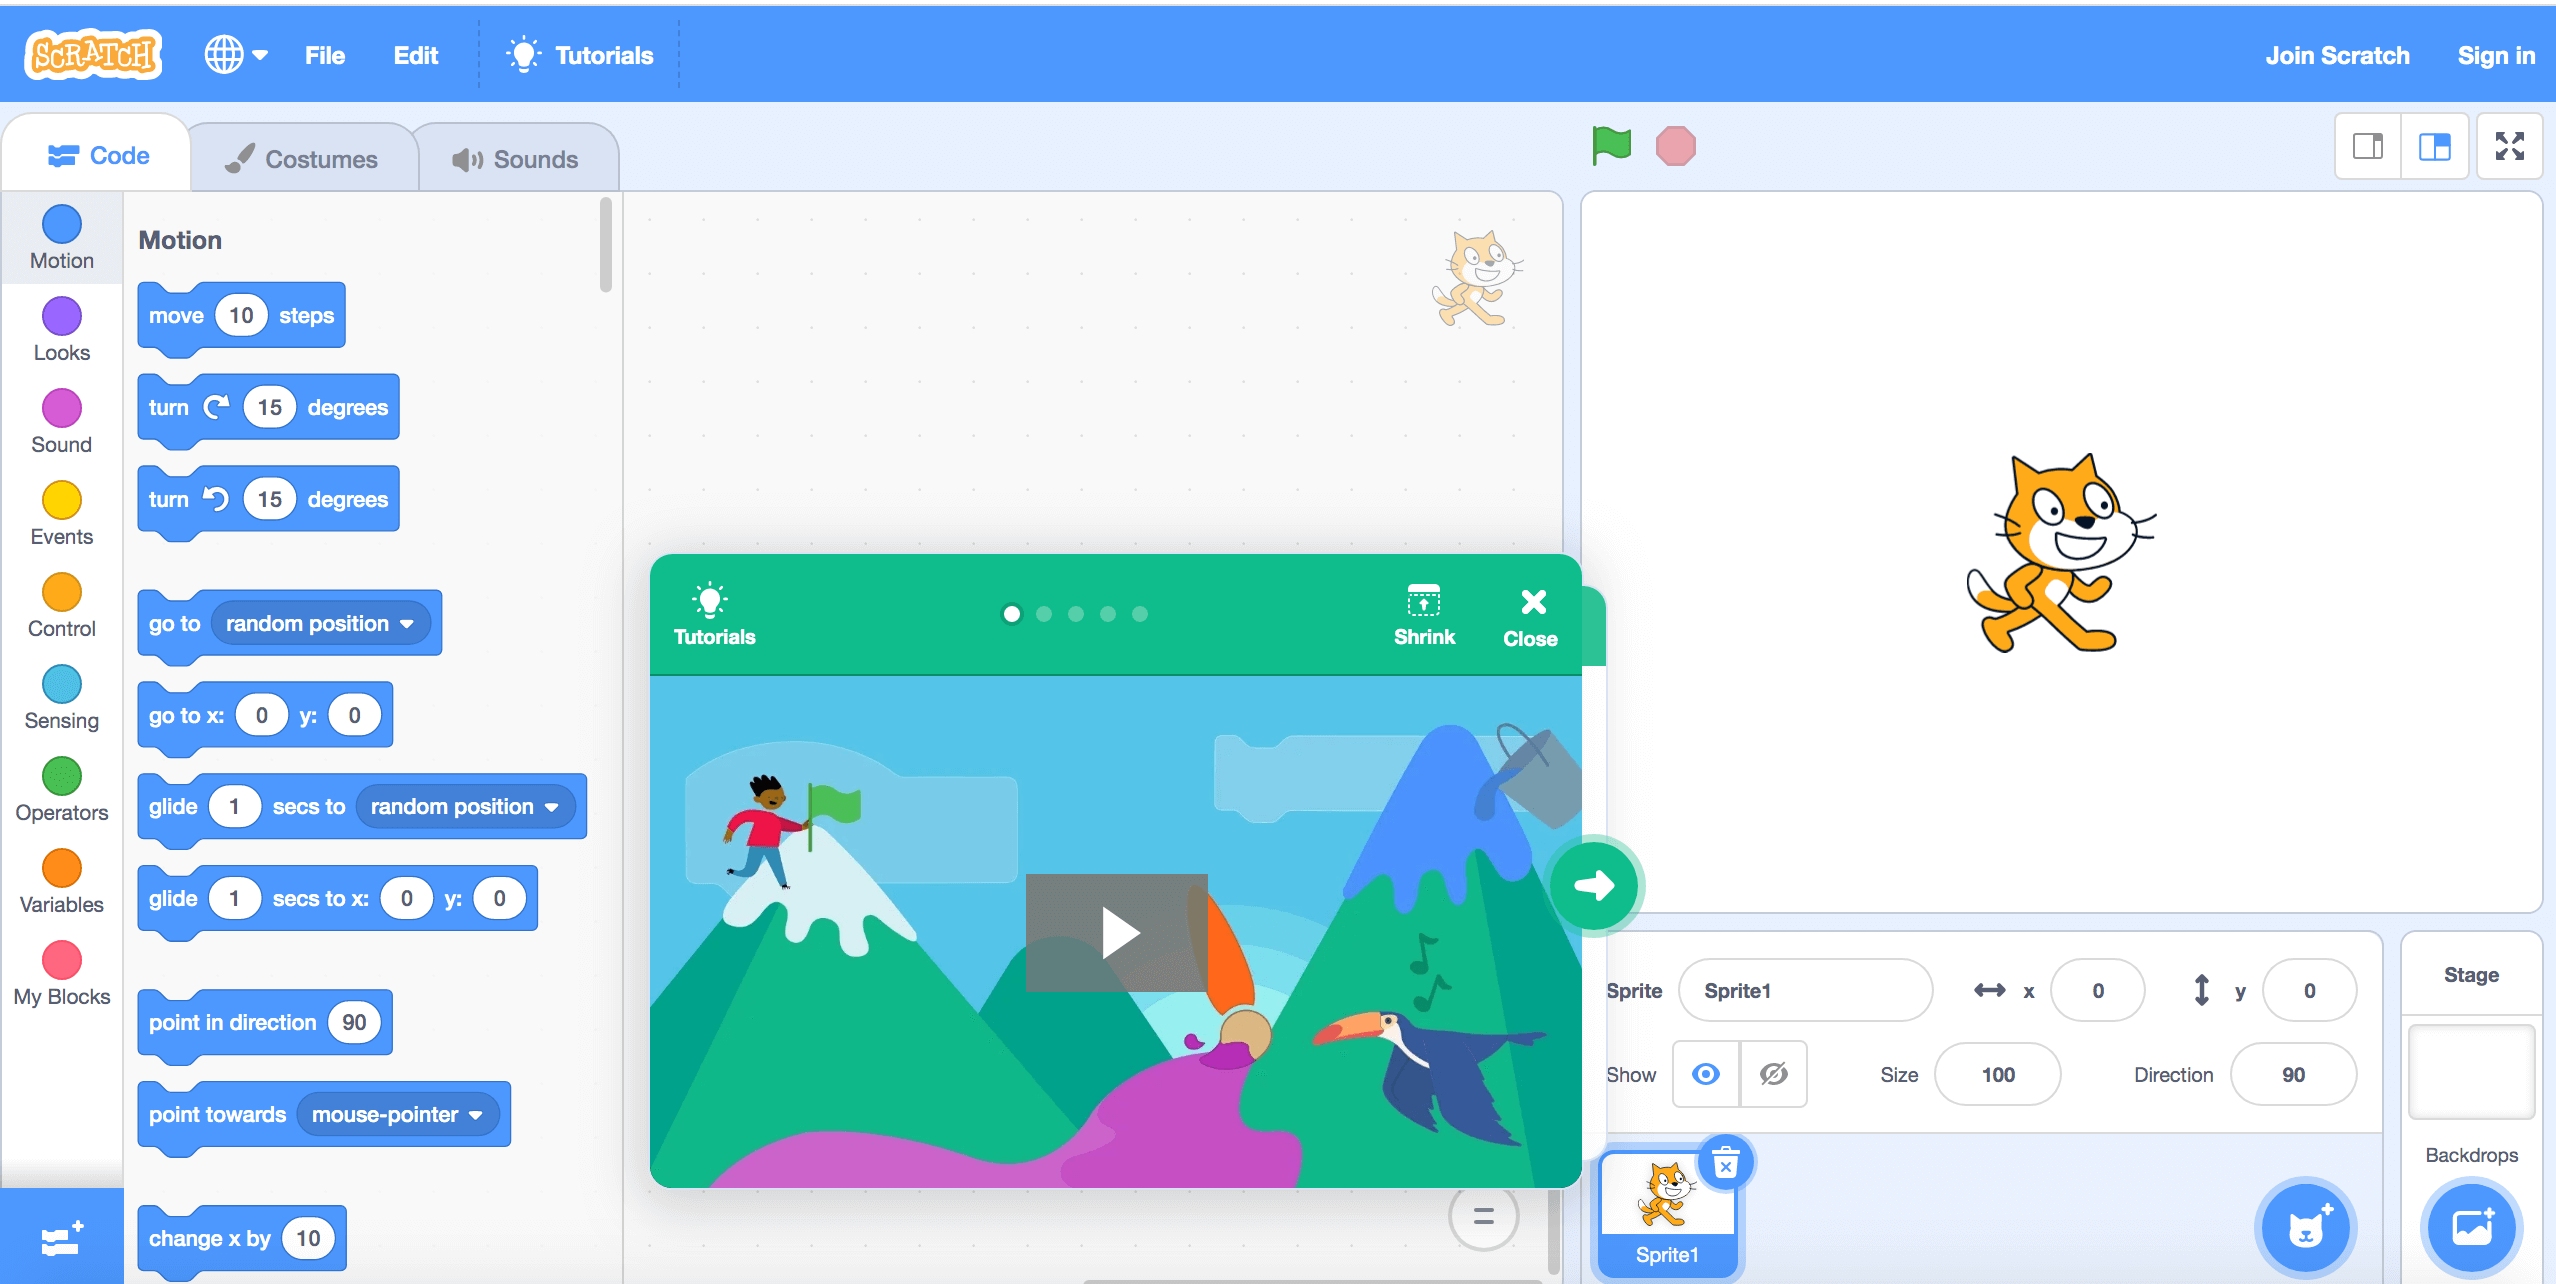
\includegraphics[width=0.8\columnwidth]{chapters/images/scratch.png}
    \caption{Scratch}
    \label{fig:my_label}
\end{figure}

Scratch es un lenguaje de programación visual basado en bloques, creado y  mantenido por Lifelong Kindergarten group en el MIT Media Lab. Scratch además es una comunidad en línea donde los niños pueden programar y compartir medios interactivos como historias, juegos y animaciones con gente de todo el mundo. Los más pequeños aprenden a pensar creativamente, trabajar en colaboración y razonar sistemáticamente\cite{scratch}. Scratch posee un lenguaje de iniciación llamado Scratch Jr pensando para niños de 5 a 7 años siendo aún más sencillo, aunque Scratch está pensado para todas las edades. Actualmente se puede utilizar desde cualquier dispositivo al ultilizar tecnologías web.

Junto con Scratch cada vez hay más plataformas y entornos STEM que se han dedicado al desarrollo de herramientas de aprendizaje enfocadas a los más pequeños. Destacan aplicaciones web como: 

\begin{itemize}
    \item  \textit{OpenRoberta \footnote{https://lab.open-roberta.org/}}: es una plataforma web creada por un instituto alemán perteneciente a la Fraunhofer Society. Tiene como objetivo simplificar conceptos de programación y facilitar a niños y profesores la codificación mediante el uso de robots como Lego Mindstorms y otros sistemas de hardware programables. \cite{openroberta}. 
    
    \begin{figure}[H]
        \centering
        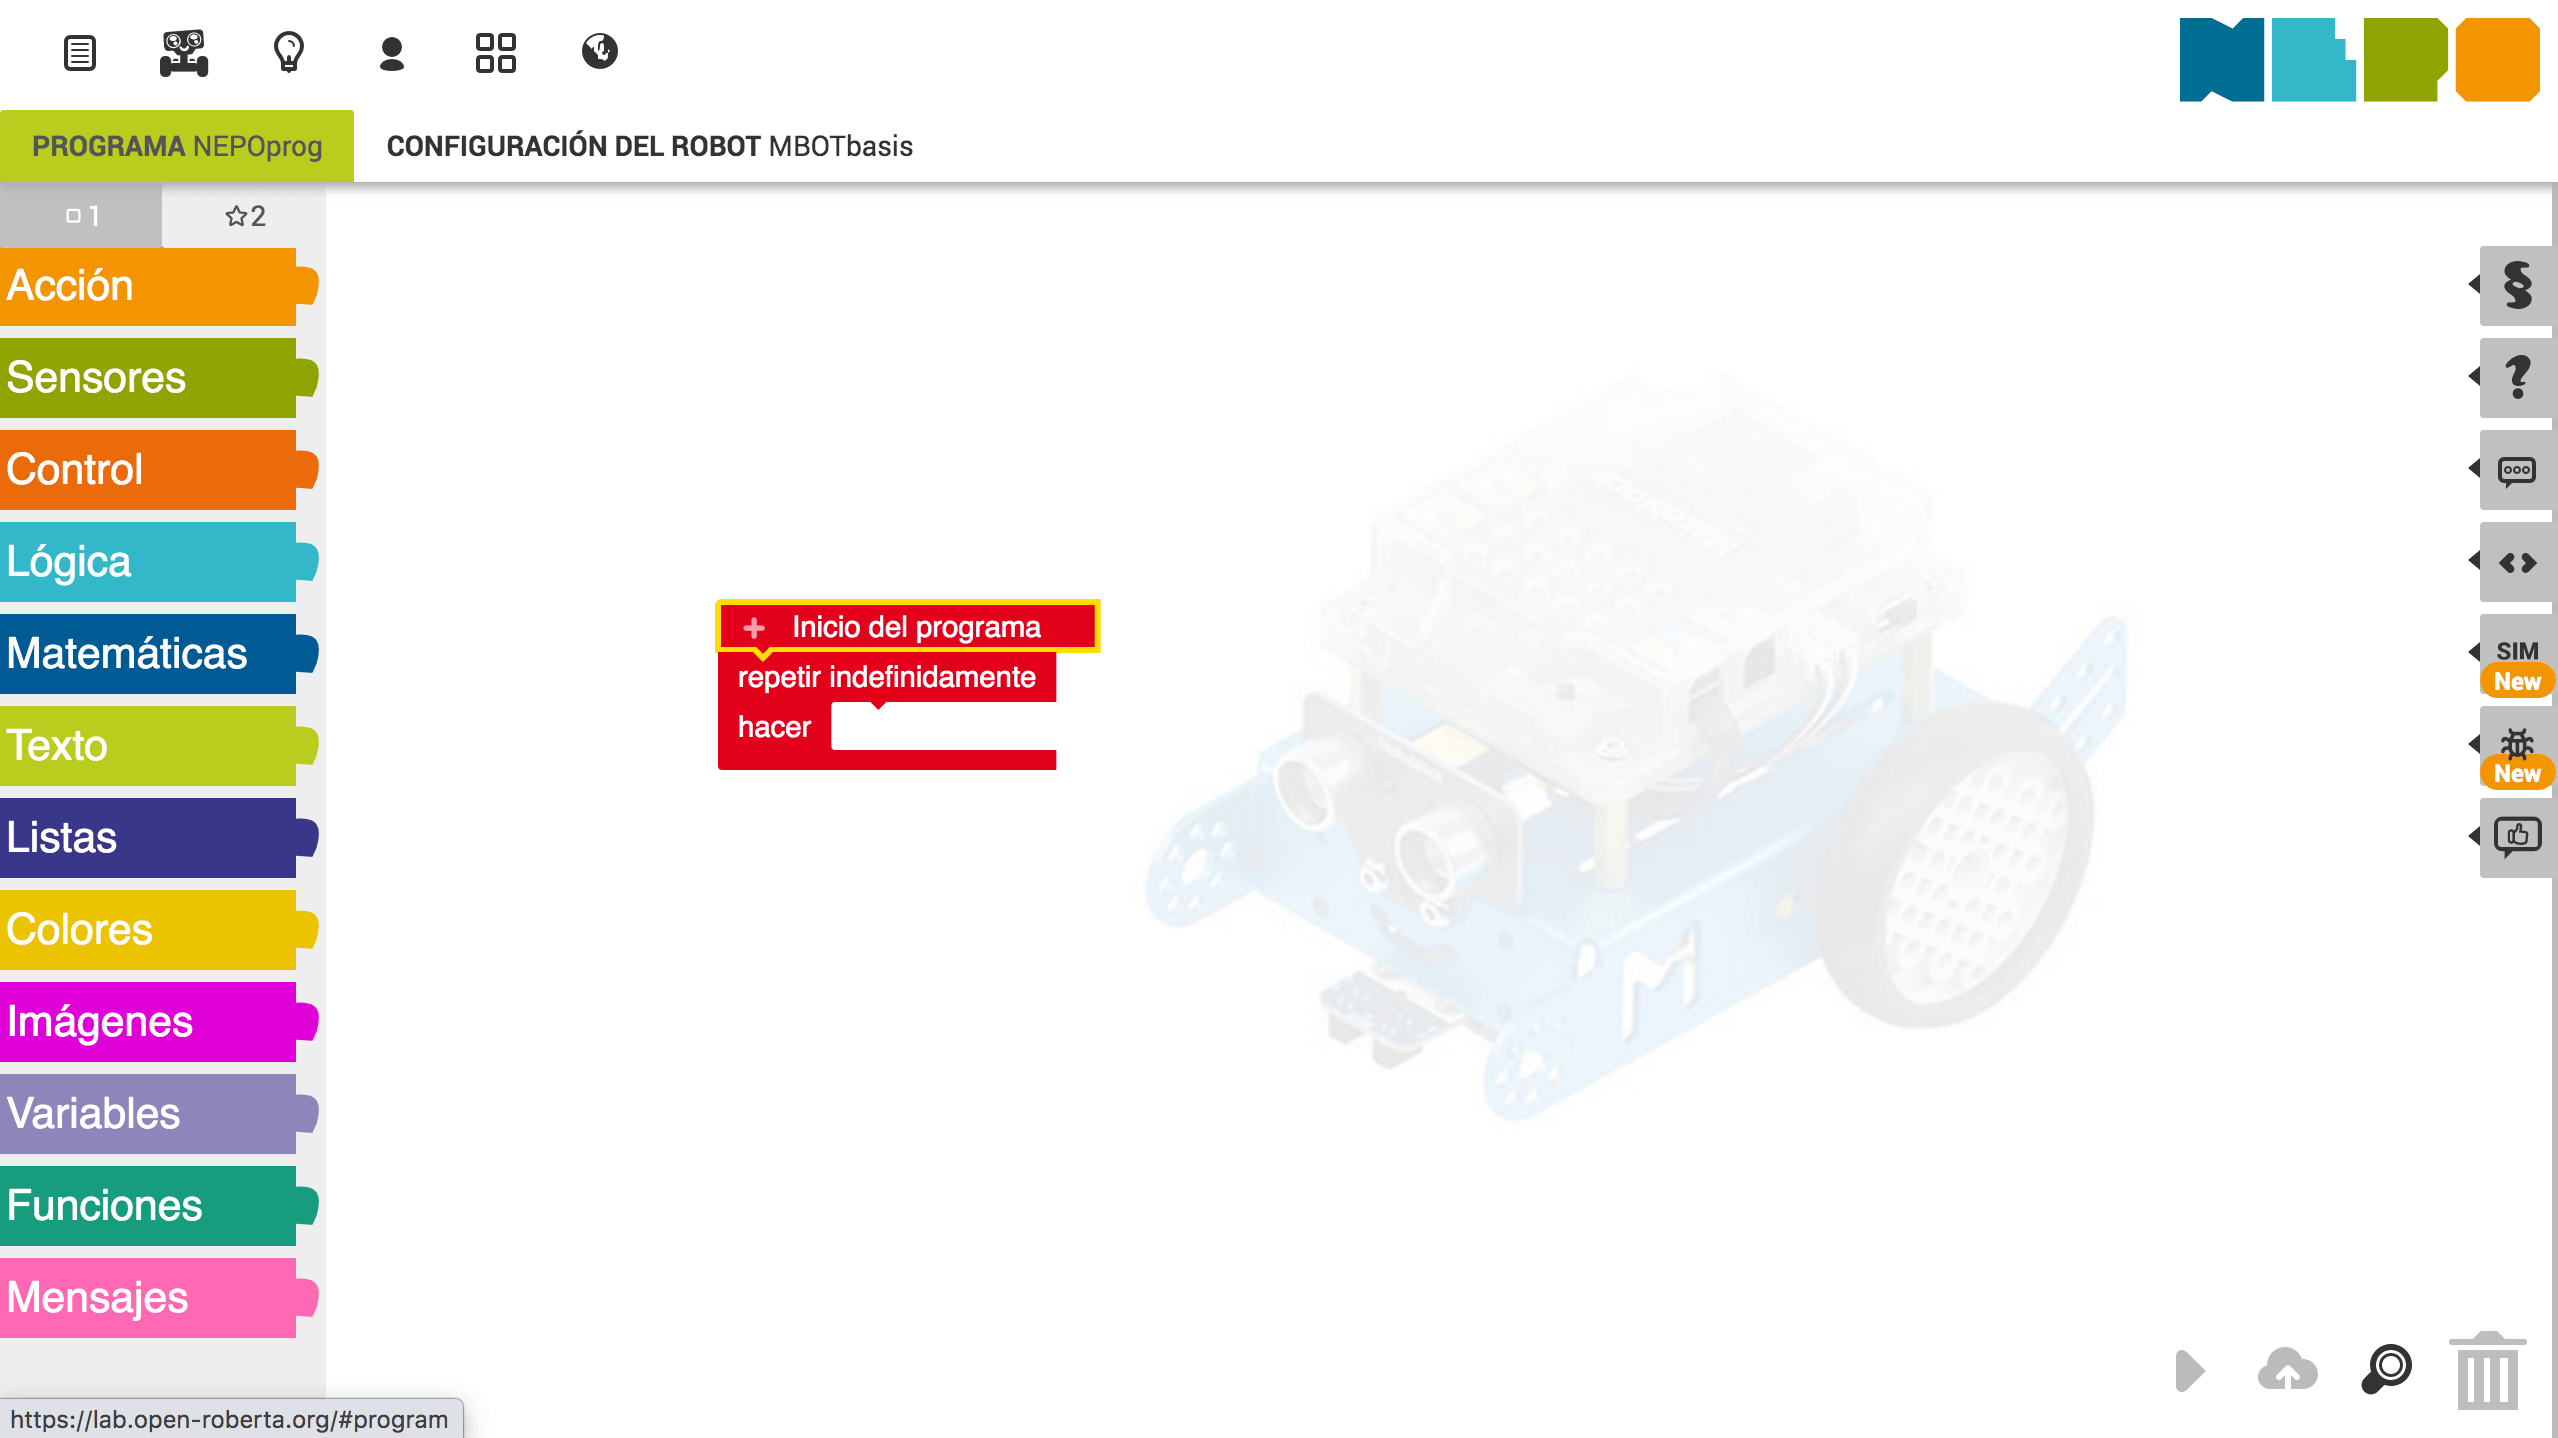
\includegraphics[width=0.7\textwidth ]{chapters/images/openrobert.png}
        \caption{Open Roberta}
        \label{fig:openroberta}
    \end{figure}
    \item \textit{LEGO Education}: la plataforma LEGO ofrece una amplia variedad de robots y \textit{packs} para uso escolar. Sus kits de robótica educativa permiten a los más pequeños construir y programar robots mediante el uso de motores, sensores, engranajes, ruedas, ejes y otros componentes técnicos, además del uso de su propio software basado en bloques. Destacan modelos como  MINDSTORMS Education EV3 y LEGO Education WeDo 2.0.\cite{ev3} \cite{legoeducation}

    \begin{figure}[H]
  \begin{subfigure}[b]{0.5\textwidth}
  \centering
    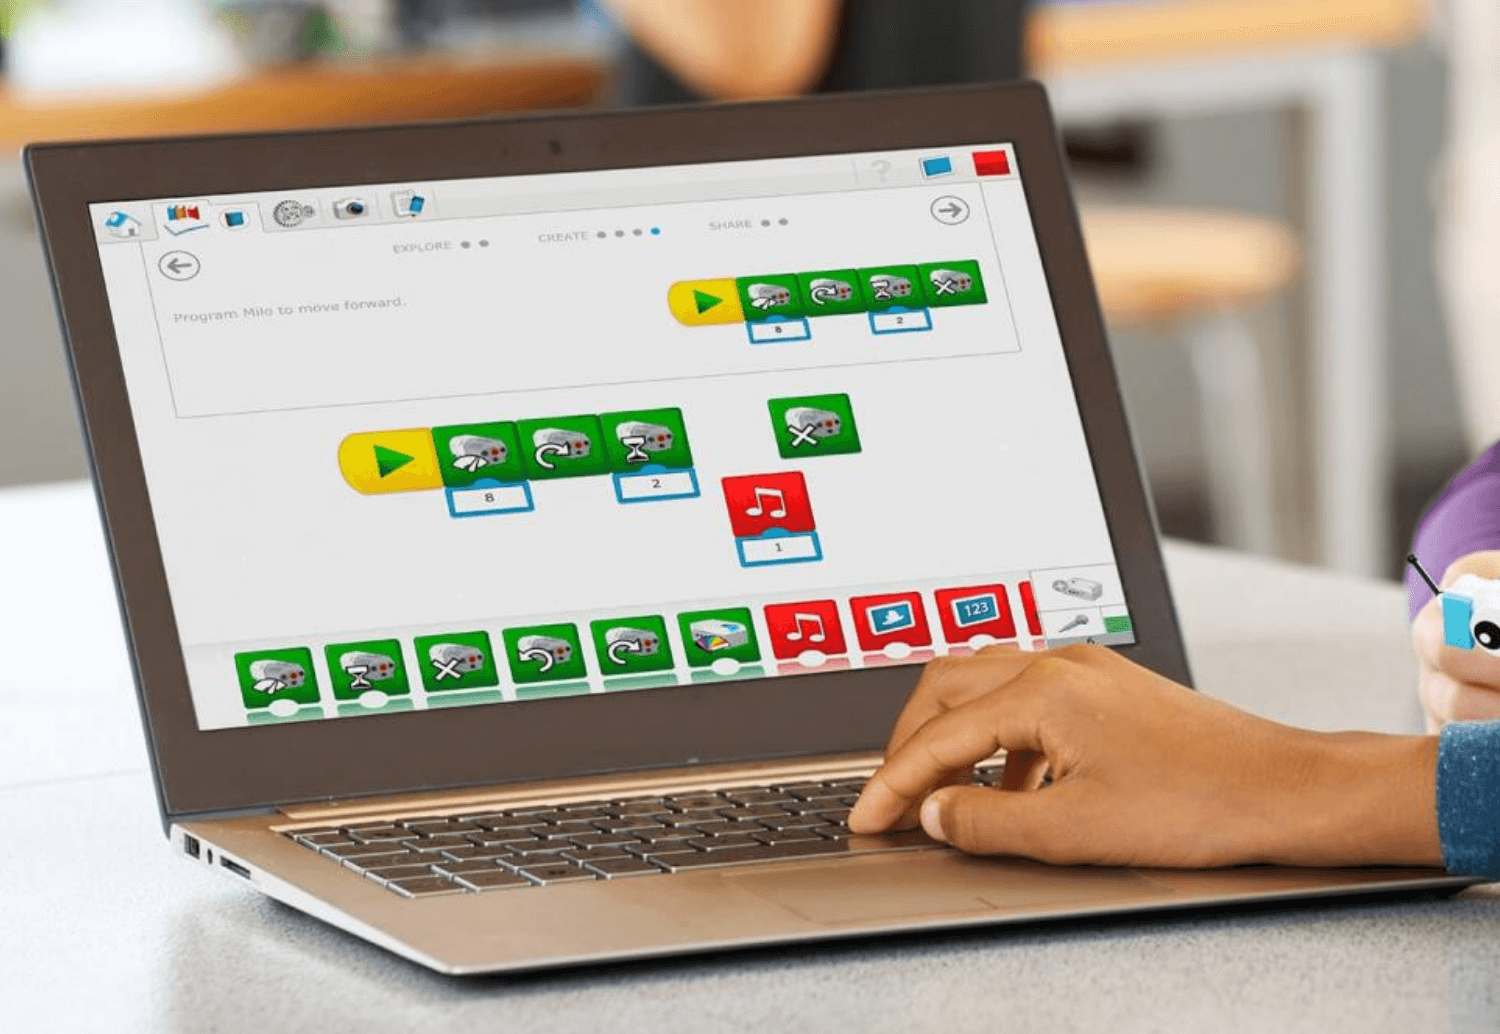
\includegraphics[width=0.9\textwidth, height=0.5\textwidth]{chapters/images/legoo.png}
    \caption{LEGO}
    \label{fig:f1}
  \end{subfigure}
  \hfill
  \begin{subfigure}[b]{0.5\textwidth}
  \centering
    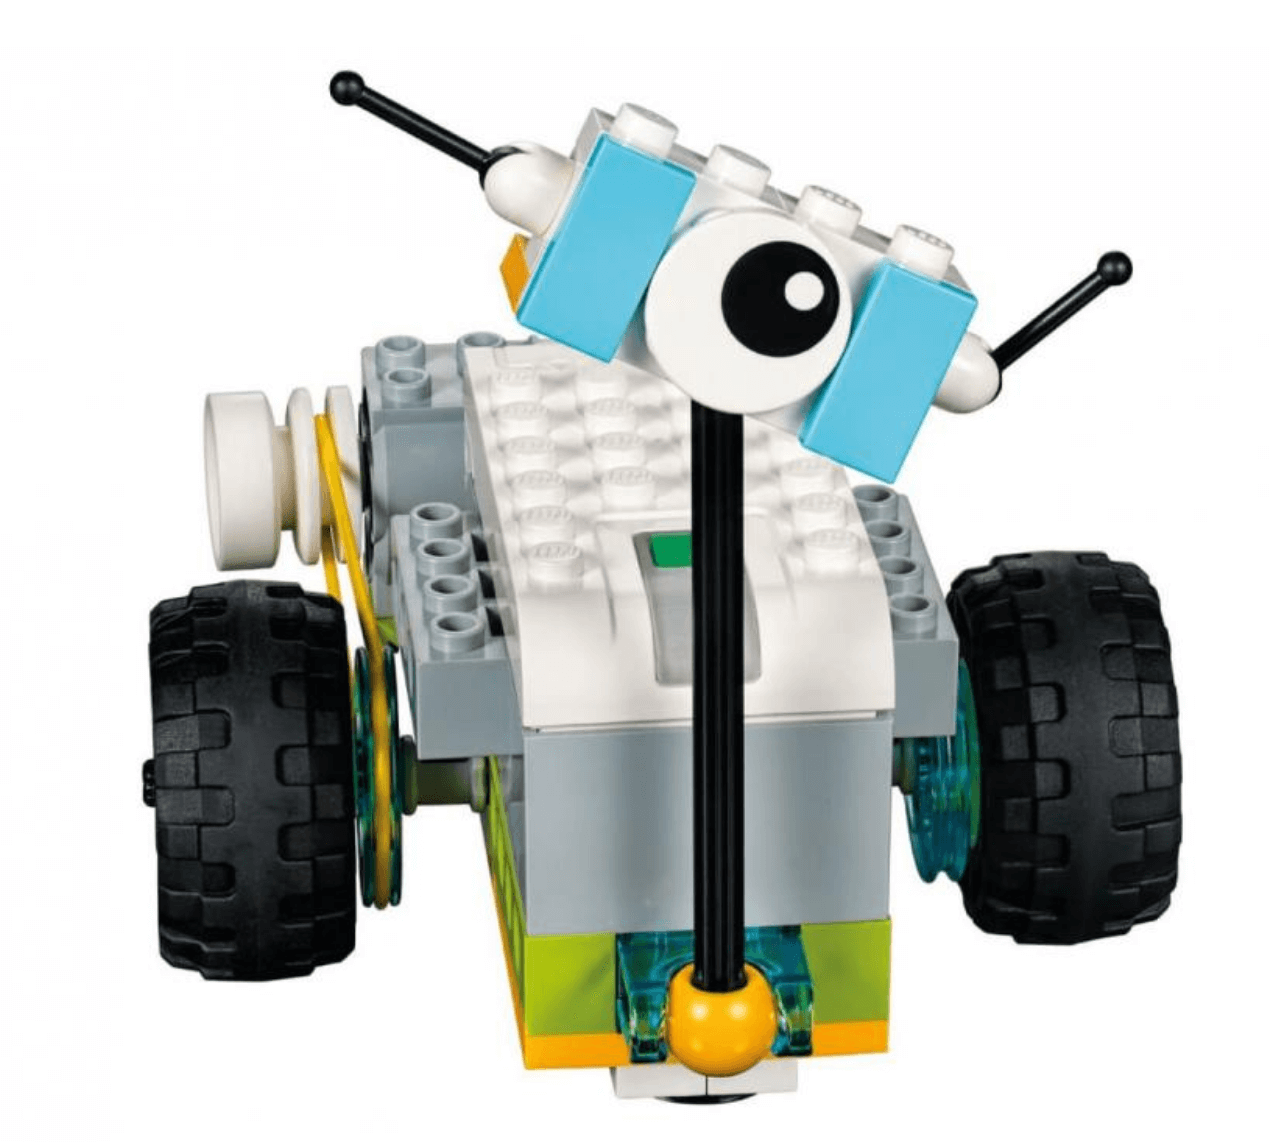
\includegraphics[width=0.9\textwidth, height=0.5\textwidth]{chapters/images/wedo.png}
    \caption{WeDo 2.0}
    \label{fig:f2}
  \end{subfigure}
  \caption{LEGO EDUCATION}
\end{figure}

    \item \textit{MBlock IDE \footnote{https://ide.mblock.cc/}}: esta aplicación web está diseñada para la educación en ciencia, tecnología, ingeniería, artes y matemáticas (STEAM). Está inspirada en Scratch 3.0, es compatible con lenguajes de programación tanto gráficos (Scratch) como textuales (Python). Se pueden diseñar historias, juegos, animaciones y programar dispositivos como robots Makeblock y microbit. \cite{mblock}
    \begin{figure}[H]
        \centering
        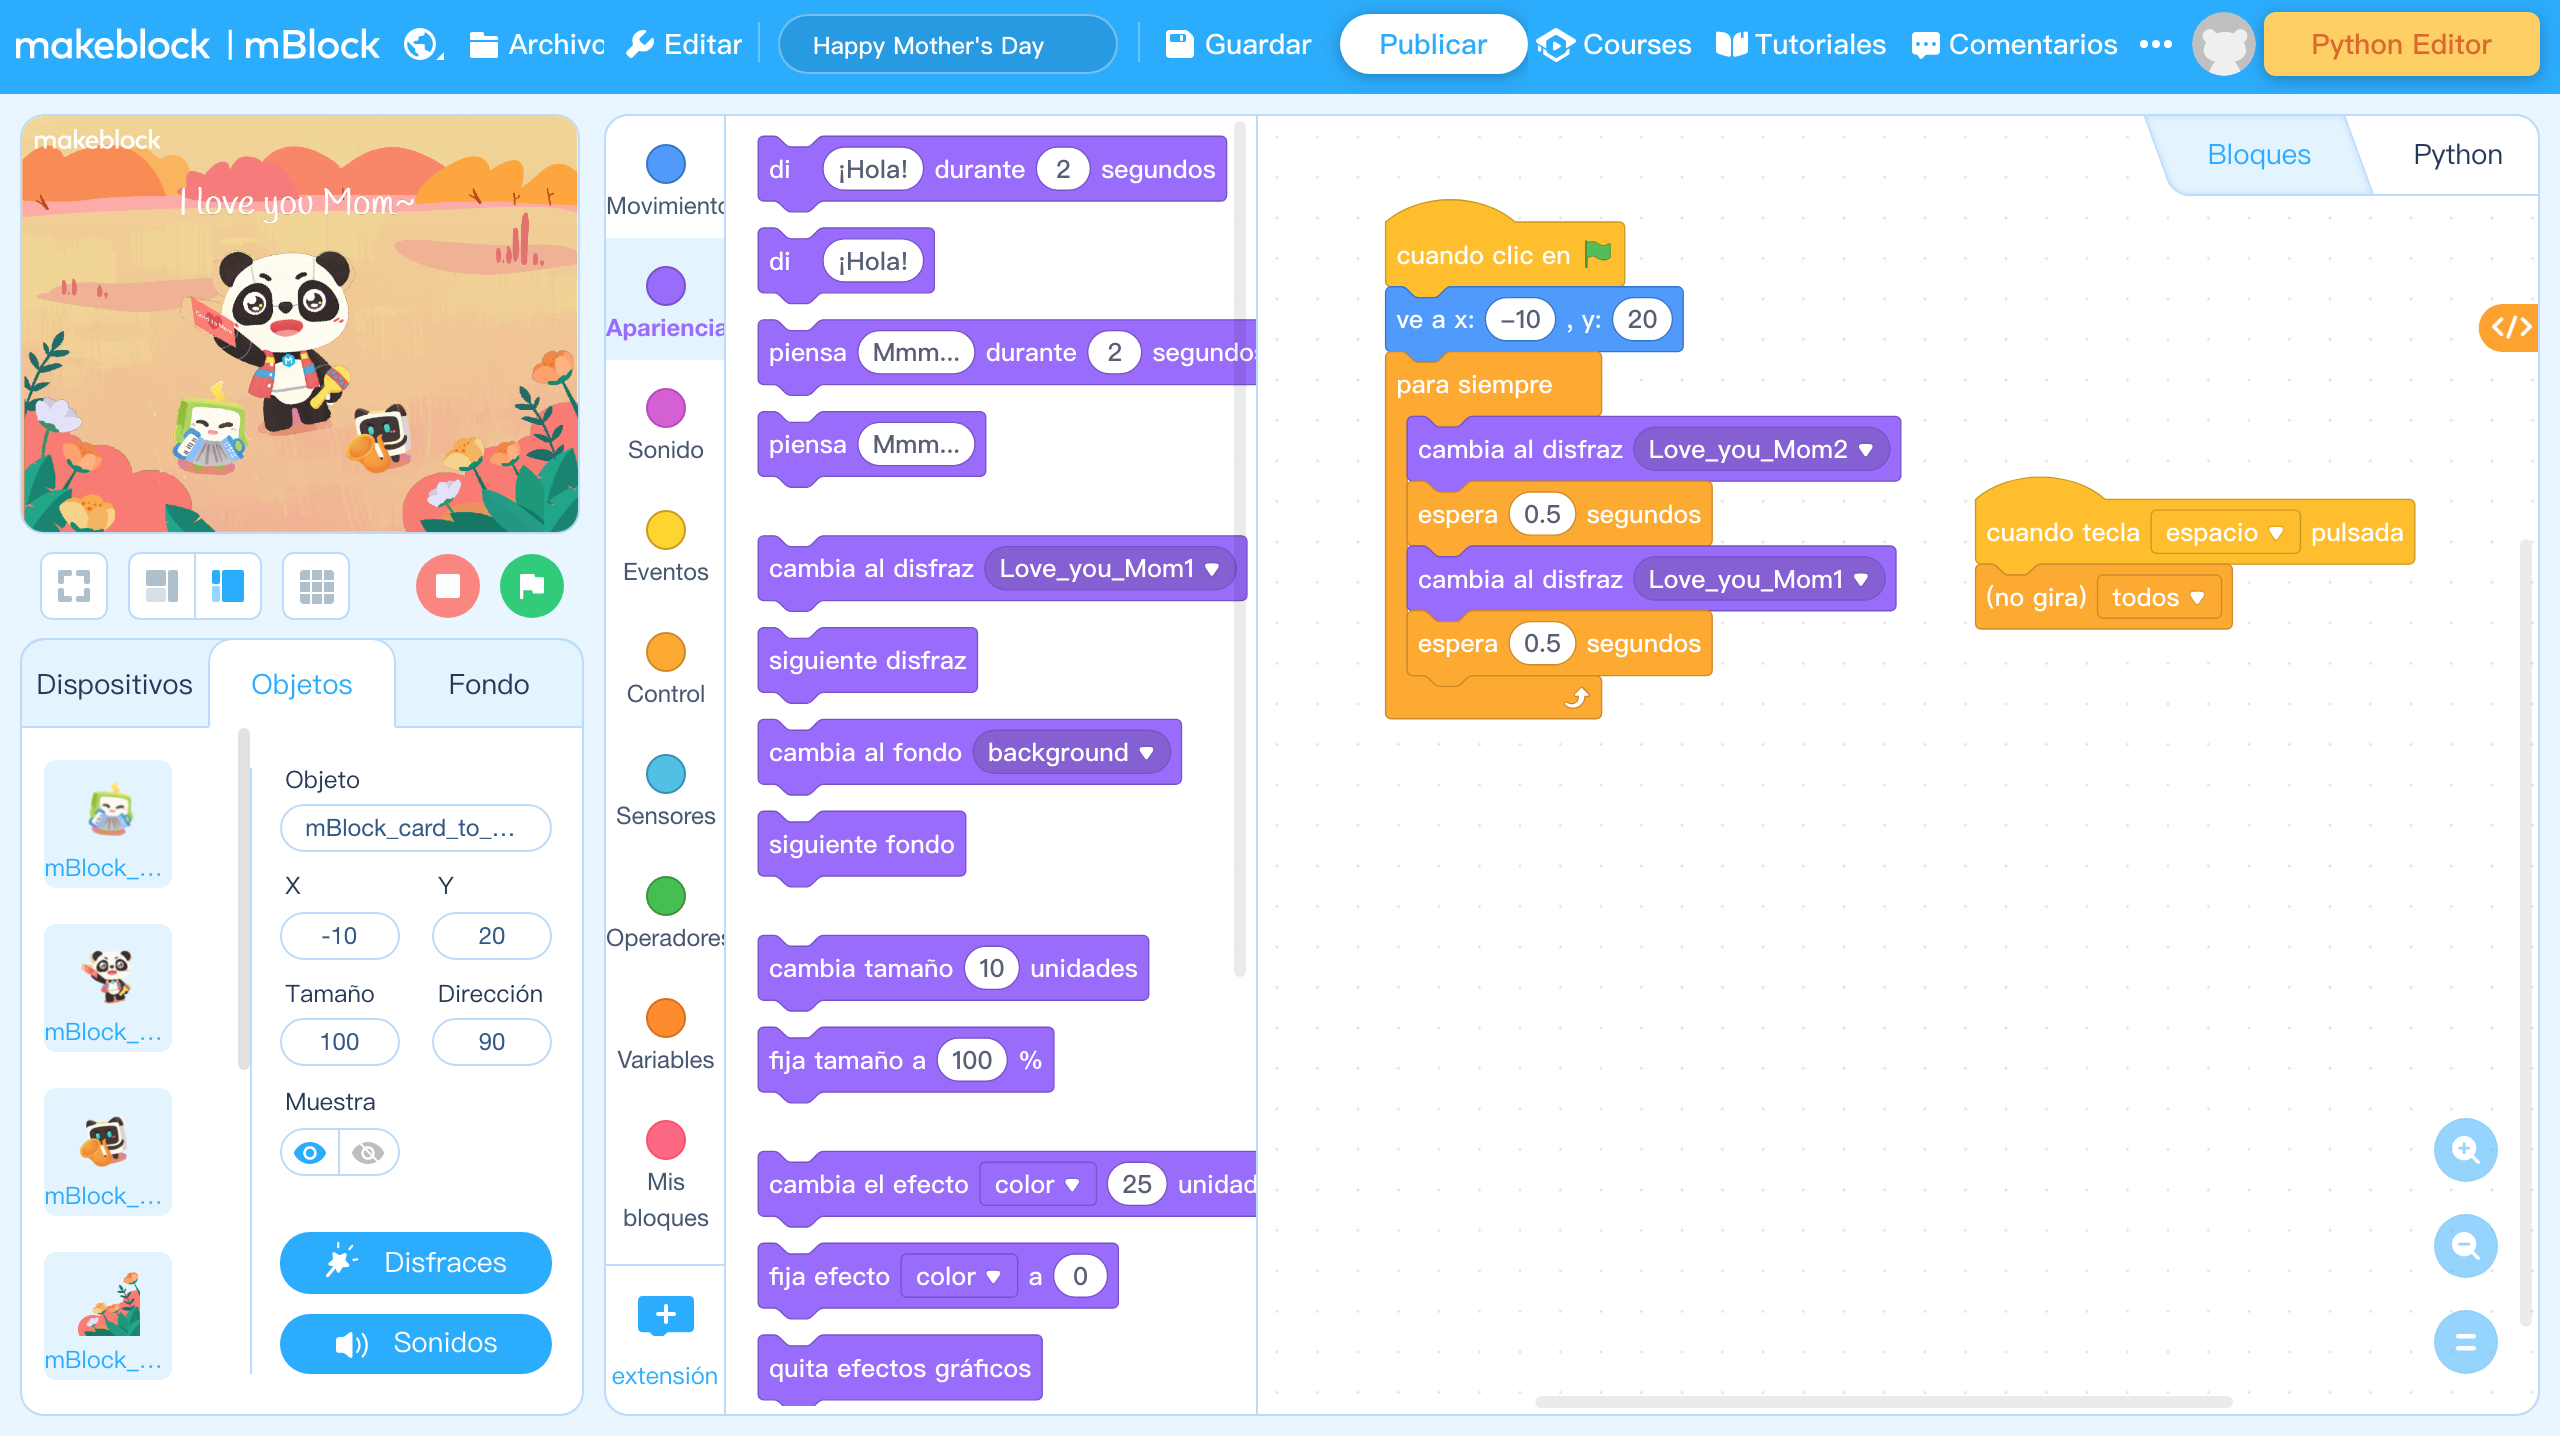
\includegraphics[width=0.7\textwidth]{chapters/images/makeblock.png}
        \caption{MBlock IDE}
        \label{fig:mblock}
    \end{figure}

    \item Vex \footnote{https://www.vexrobotics.com/}, AppInventor \footnote{https://appinventor.mit.edu/}, Arduino Web Editor\footnote{https://store.arduino.cc/digital/create}, Kodu \footnote{http://www.kodugamelab.com/} o Snap! \footnote{https://snap.berkeley.edu/} son otras plataformas web de programación en robótica educativa.
\end{itemize}


La plataforma de robótica educativa que vamos utilizar en este TFG es Kibotics. Esta plataforma, basada en tecnologías web, enseña de manera atractiva conceptos básicos de tecnología e inicia a niños y adolescentes en robótica y programación. Sigue un enfoque práctico, fomentando el pensamiento y la organización para resolver un problema, además de formar el espíritu analítico de los alumnos \cite{intro}.
\\
Actualmente ofrece cursos de robótica en Scratch y Python (Figura 1.16). En el capítulo 3 se ampliará información sobre Kibotics y veremos cómo se introduce la \textit{Gamificación} en la plataforma a lo largo de este trabajo.

\begin{figure}[H]
  \begin{subfigure}[b]{0.5\textwidth}
  \centering
    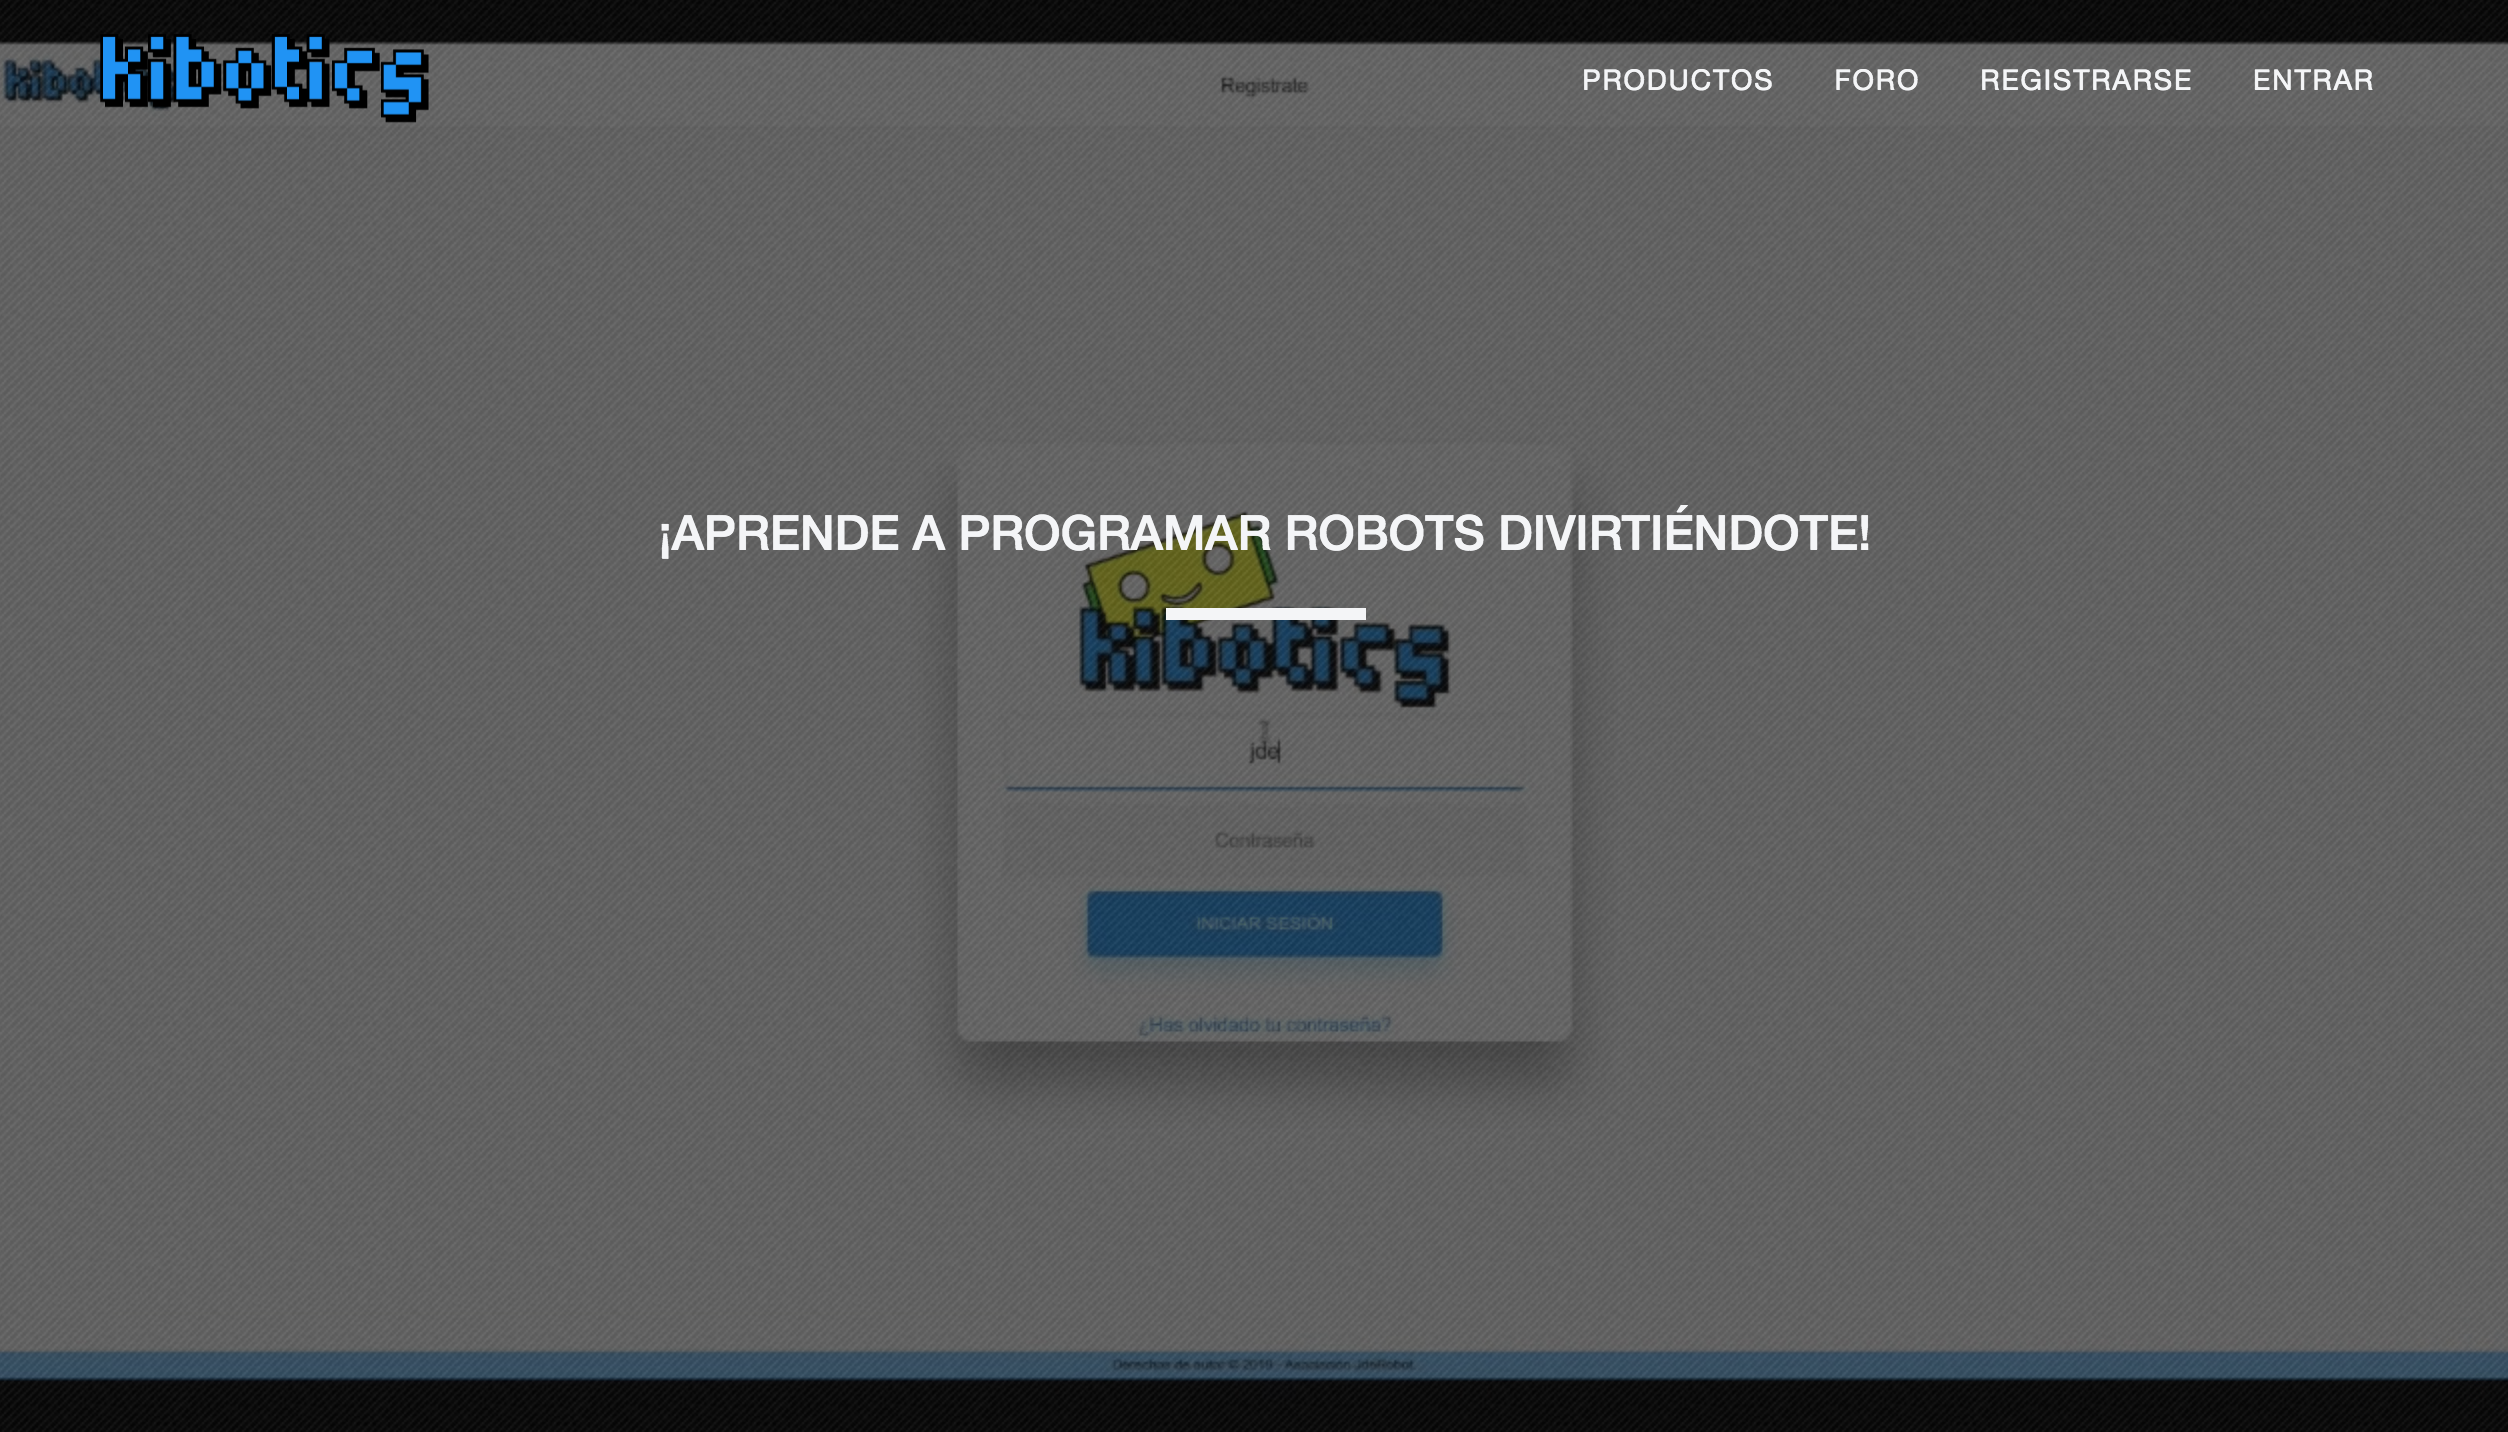
\includegraphics[width=0.9\textwidth, height=0.6\textwidth]{chapters/images/kiboticsorg.png}
    \caption{kibotics.org}
    \label{fig:f1}
  \end{subfigure}
  \hfill
  \begin{subfigure}[b]{0.5\textwidth}
  \centering
    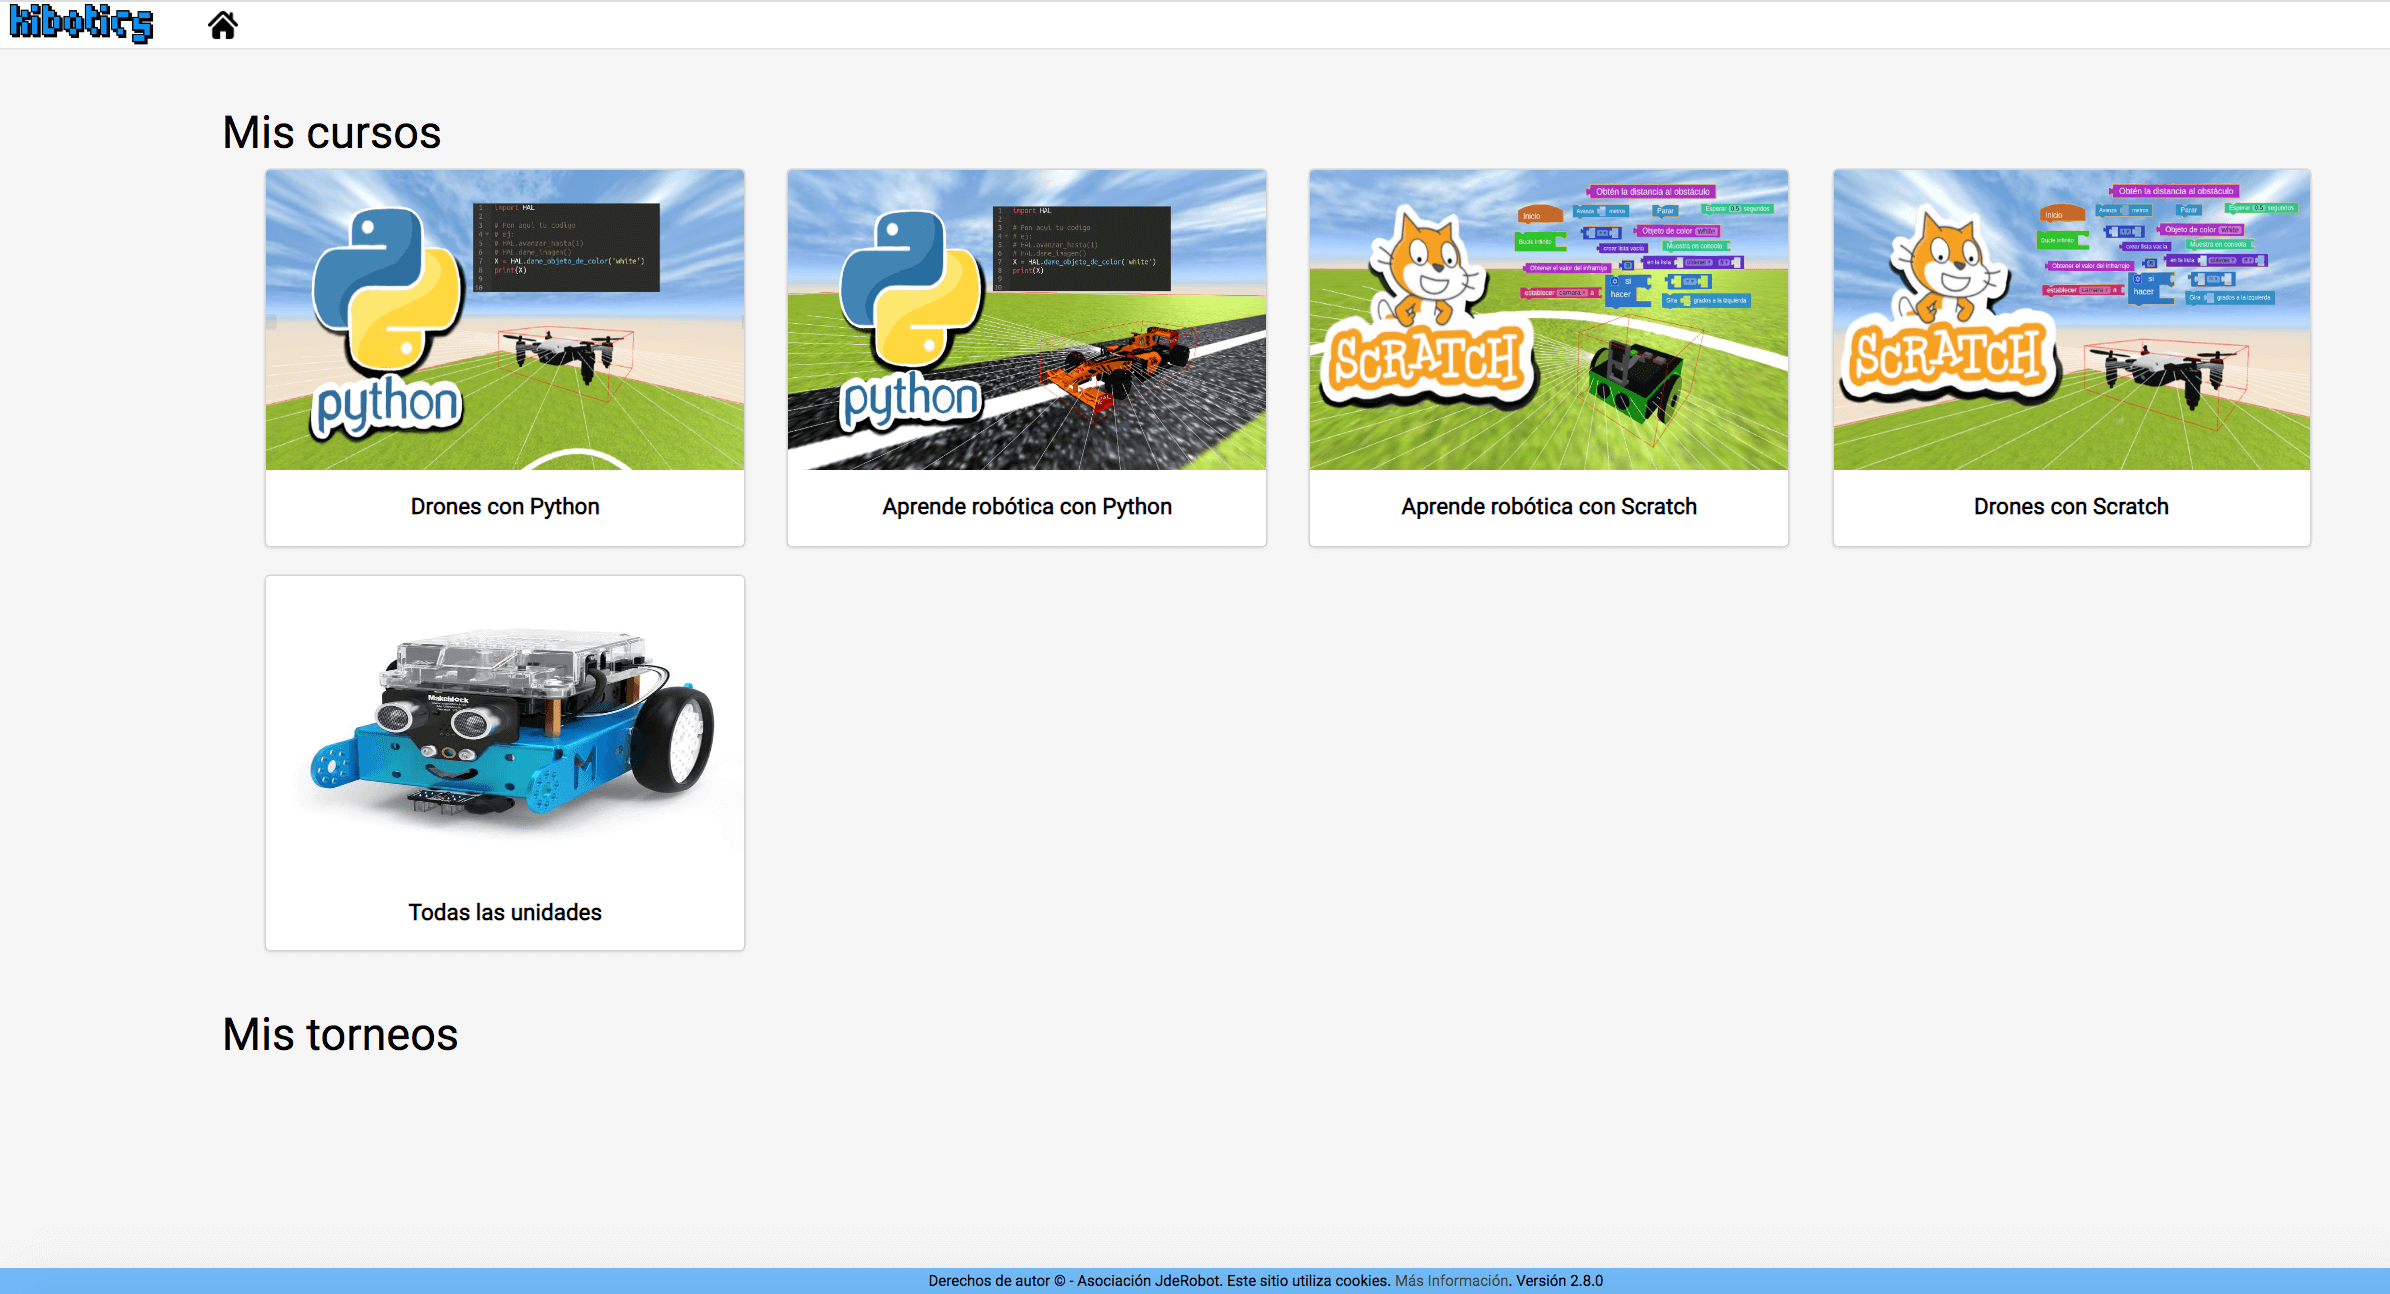
\includegraphics[width=0.9\textwidth, height=0.6\textwidth]{chapters/images/kibotics.png}
    \caption{Cursos disponibles en Kibotics.}
    \label{fig:f2}
  \end{subfigure}
  \caption{Plataforma Kibotics.}
\end{figure}
 
\subsection{Importancia de los juegos y multimedia en el aprendizaje} 
El planteamiento actual del sistema educativo tiene carencias y la innovación en la educación cobra cada vez más importancia. Es por ello que los docentes buscan actividades enfocadas en evitar la recurrente pasividad de los alumnos\cite{multimedia}.

Según concluyen el cono del aprendizaje de Edgar Dale y otros estudios, aprendemos un 10\% de lo que leemos, 20\% de lo que escuchamos, 75\% de lo que vemos y oimos y 
90\% de lo que hacemos \cite{videoeducativo}\cite{aprendizaje}. Estos porcentajes indican que, por lo tanto, la introducción del vídeo y los juegos interactivos en la clase puede producir modificaciones primordiales en el ámbito educativo.

La multimedia es un valioso recurso en la enseñanza por su naturaleza interactiva. Estos  materiales  deben ser adecuados y facilitar el aprendizaje. Para eso deben ser de fácil instalación y uso, versátiles, mostrar información de calidad e interactivos para motivar a los alumnos. Cada material se ajusta a los usuarios para que cada uno  trabaje a su ritmo \cite{importanciamultimedia}.
\\
Las nuevas tecnologías están cada vez más interiorizadas en las aulas gracias al uso de pantallas, proyectores y ordenadores. La pandemia vivida en este último año ha impulsado el uso de aplicaciones web para dar clase, como las plataformas de videoconferencia. Muchos profesores han optado por estas potentes plataformas, otros han grabado y compartido sus propios vídeos, donde los estudiantes pueden pararlos y verlos las veces necesarias para interiorizar mejor los conocimientos.
\\
En los últimos años se están incorporando juegos en las aulas como la apliación Kahoot! \cite{kahoot} en la que hacen juegos de encuestas, además se ha fomentado aprendizaje a través de vídeos y diapositivas más animadas, foros, así como el uso de plataformas educativas e interactivas como Moodle.
\\

 El término \textit{``Gamificación''} o ludificación se emplea para referirse al aprendizaje a través de juegos en el entorno educativo y profesional. Los juegos se utilizan para fomentar el aprendizaje de programación, mejorando los conocimientos y habilidades de los alumnos de una forma más dinámica y divertida. La Gamificación facilita la interiorización de los conocimientos, generando una respuesta positiva al usuario por cumplir con un objetivo.
 \\
 Enseñar a los más jóvenes cómo funcionan las últimas tecnologías y que además les parezca entretenido e interesante es lo que nos ha motivado a realizar este trabajo.
 
 
\subsection{Campeonatos de robótica educativa existentes}

El aprendizaje de la robótica educativa ha ido más allá. Actualmente existen competiciones a nivel nacional e internacional que utilizan juegos y ejercicios competitivos \cite{competiciones}. Estas son algunas de ellas:
\begin{itemize}
    \item RoboCup Junior \footnote{https://junior.robocup.org/}: es una iniciativa educativa orientada a proyectos que patrocina eventos robóticos locales, regionales e internacionales para jóvenes estudiantes. Destaca la Liga de Rescate, Liga de Futbol (Figura 1.17(b)) y Liga ONSTAGE \cite{robocup}.
 
    \item Eurobot Junior\footnote{http://www.eurobot.es/}: es una competición europea de robots para estudiantes de primaria, secundaria o clubs de robótica. El grupo de jóvenes debe diseñar, construir y programar un robot telecontrolado por cable. Además pueden tener un robot secundario autónomo\cite{eurobot}.
    
    \item First Lego league \footnote{https://www.firstlegoleague.es/}: es un programa internacional  para jóvenes de 4 a 16 años a través de la resolución de problemas reales. Se adapta a cada edad con sus cursos Discover, Explore y Challenge\cite{firstlego}.
    
    \item Torneo Nacional VEX Robotics IQ\footnote{https://vexspain.com/}: destinado a equipos de 4 a 8 miembros de secundaria junto un adulto. Ofrecen distintos retos y torneos con premios\cite{vex}.
    
    \item RoboCampeones \footnote{http://robocampeones.org/}: Creado en el RoboticsLabURJC de la Universidad Rey Juan Carlos. Los alumnos de instituto compiten en pruebas como sumo con robots LEGO y Arduino. Se celebra en Fuenlabrada y en los últimos años contó con más de 2000 participantes (Figura 1.17(a)) \cite{robocampeones}.
    \\
    \\
    
    \begin{figure}[H]
  \begin{subfigure}[b]{0.5\textwidth}
  \centering
    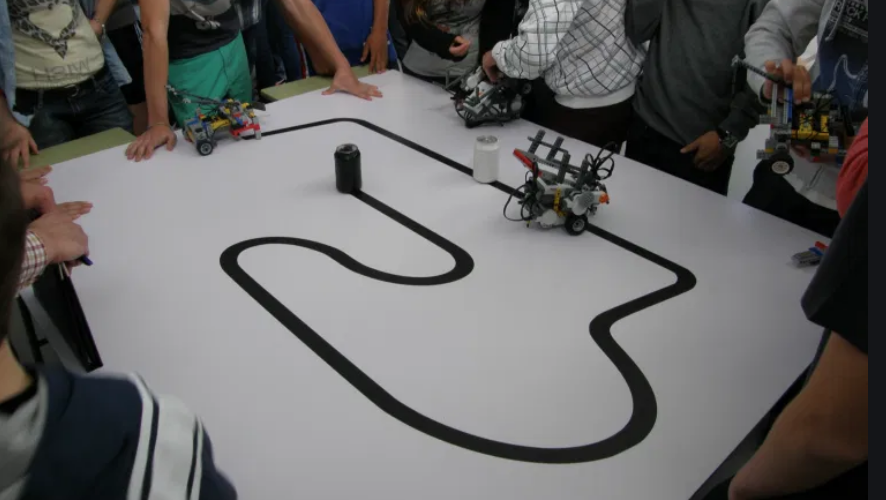
\includegraphics[width=0.95\textwidth, height=0.7\textwidth]{chapters/images/robocam.png}
    \caption{Juego Pañuelo Robocampeones}
    \label{fig:f1}
  \end{subfigure}
  \hfill
  \begin{subfigure}[b]{0.5\textwidth}
  \centering
    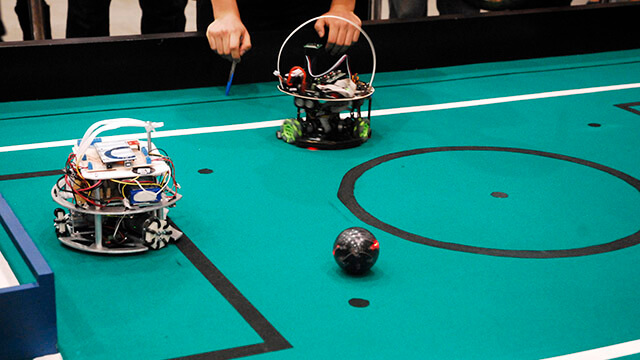
\includegraphics[width=0.95\textwidth, height=0.7\textwidth]{chapters/images/robocup.jpeg}
    \caption{Fútbol en RoboCup Junior.}
    \label{fig:f2}
  \end{subfigure}
  \caption{Campeonatos de robótica.}
\end{figure}
\end{itemize}

\newpage
\section{Estructura del documento}

La estructura de este trabajo fin de grado está compuesta por los siguientes capítulos:

\begin{itemize}
    \item \textit{Capítulo 1 Introducción}: una breve introducción a la robótica y tecnologías web para ponernos en contexto y presentar el tema principal del trabajo.
    \item \textit{Capítulo 2 Objetivos y Metodología}: Se fijan los objetivos concretos y se explica la metodología y plan de trabajo seguidos a lo largo de este proyecto.
    \item \textit{Capítulo 3 Infraestuctura utilizada}: se describen lenguajes, tecnologías y herramientas empleadas en este trabajo.
\end{itemize}

Para una mejor exposición del trabajo que se ha realizado, el desarrollo se ha dividido en 3 Capítulos. De esta forma nos centraremos en el enunciado, la infraestructura y solución de referencia de cada ejercicio:
    
\begin{itemize}
   \item \textit{Capítulo 4 Ejercicio Teleoperador Acústico y Banda Sonora}
    \item \textit{Capítulo 5 Ejercicio Aspiradora robótica atrapa confeti}
    
    \item \textit{Capítulo 6 Ejercicio Juego del pañuelo}

    
    \item \textit{Capítulo 7 Conclusiones y trabajos futuros}: Conclusiones del trabajo y futuros proyectos posibles a partir de éste.
  \end{itemize}


% OBJETIVOS 
%%%%%%%%%%%%%%%%%%%%%%%%%%%%%%%%%%%%%%%%%%%%%%%%%%%%%%%%%%%%%%%%%%%%%%%%%%%%%%%%
\chapter{Objetivos y Metodología del Trabajo}\label{objetivos}

En este capítulo se plantean los objetivos a cumplir con este proyecto, así como los requisitos, metodología y el plan de trabajo que se ha seguido para alcanzarlos.

\section{Objetivos}

El objetivo principal de este trabajo es introducir la gamificación en la plataforma Kibotics, para ello, vamos a centrarnos en los siguientes subobjetivos u objetivos específicos a cumplir:

\begin{itemize}
    \item Diseñar y desarrollar un nuevo juego que analice el audio en tiempo real y explorar la posibilidad de añadir bandas sonoras a los ejercicios actuales. 

    \item Diseñar y desarrollar un nuevo ejercicio sobre una aspiradora robótica que tiene que limpiar una habitación.

    \item Diseñar y desarrollar un nuevo ejercicio sobre un robot que juega al pañuelo, recorriendo una línea, una lata que ejerce de pañuelo y regresando con ella al lugar de partida.

    Para los tres ejercicios se desarrollará la infraestructura necesaria, modelos nuevos de robot, escenarios en el simulador, evaluadores automáticos, soluciones de referencia y se integrarán en la plataforma web de robótica eduactiva Kibotics.
    
\end{itemize}


\newpage

\section{Requisitos}
Para cumplir con los objetivos citados anteriormente debemos tener en cuenta además los siguientes  requisitos: 
\begin{itemize}
    \item Los robots y juegos desarrollados deben ser compatibles con la versión actual v.2.8 o superior de Kibotics.
    \item No se debe requerir de instalaciones adicionales. Todo debe correr en el navegador web del cliente. 
    \item Uso de software de simulación Websim y A-Frame.
\end{itemize}

 
\section{Metodología}

La metodología que se ha seguido para la realización de este trabajo es la basada en el modelo de desarrollo software iterativo y creciente (Figura 2.1) \cite{modeloiter}.
Este modelo consiste en entregar a los usuarios y al equipo de desarrolladores de Kibotics, una versión usable lo antes posible y en continua actualización. En cada iteración se van solventando pequeños errores y mejoras que convergen en la versión final del proyecto.

\begin{figure}[H]
    \centering
    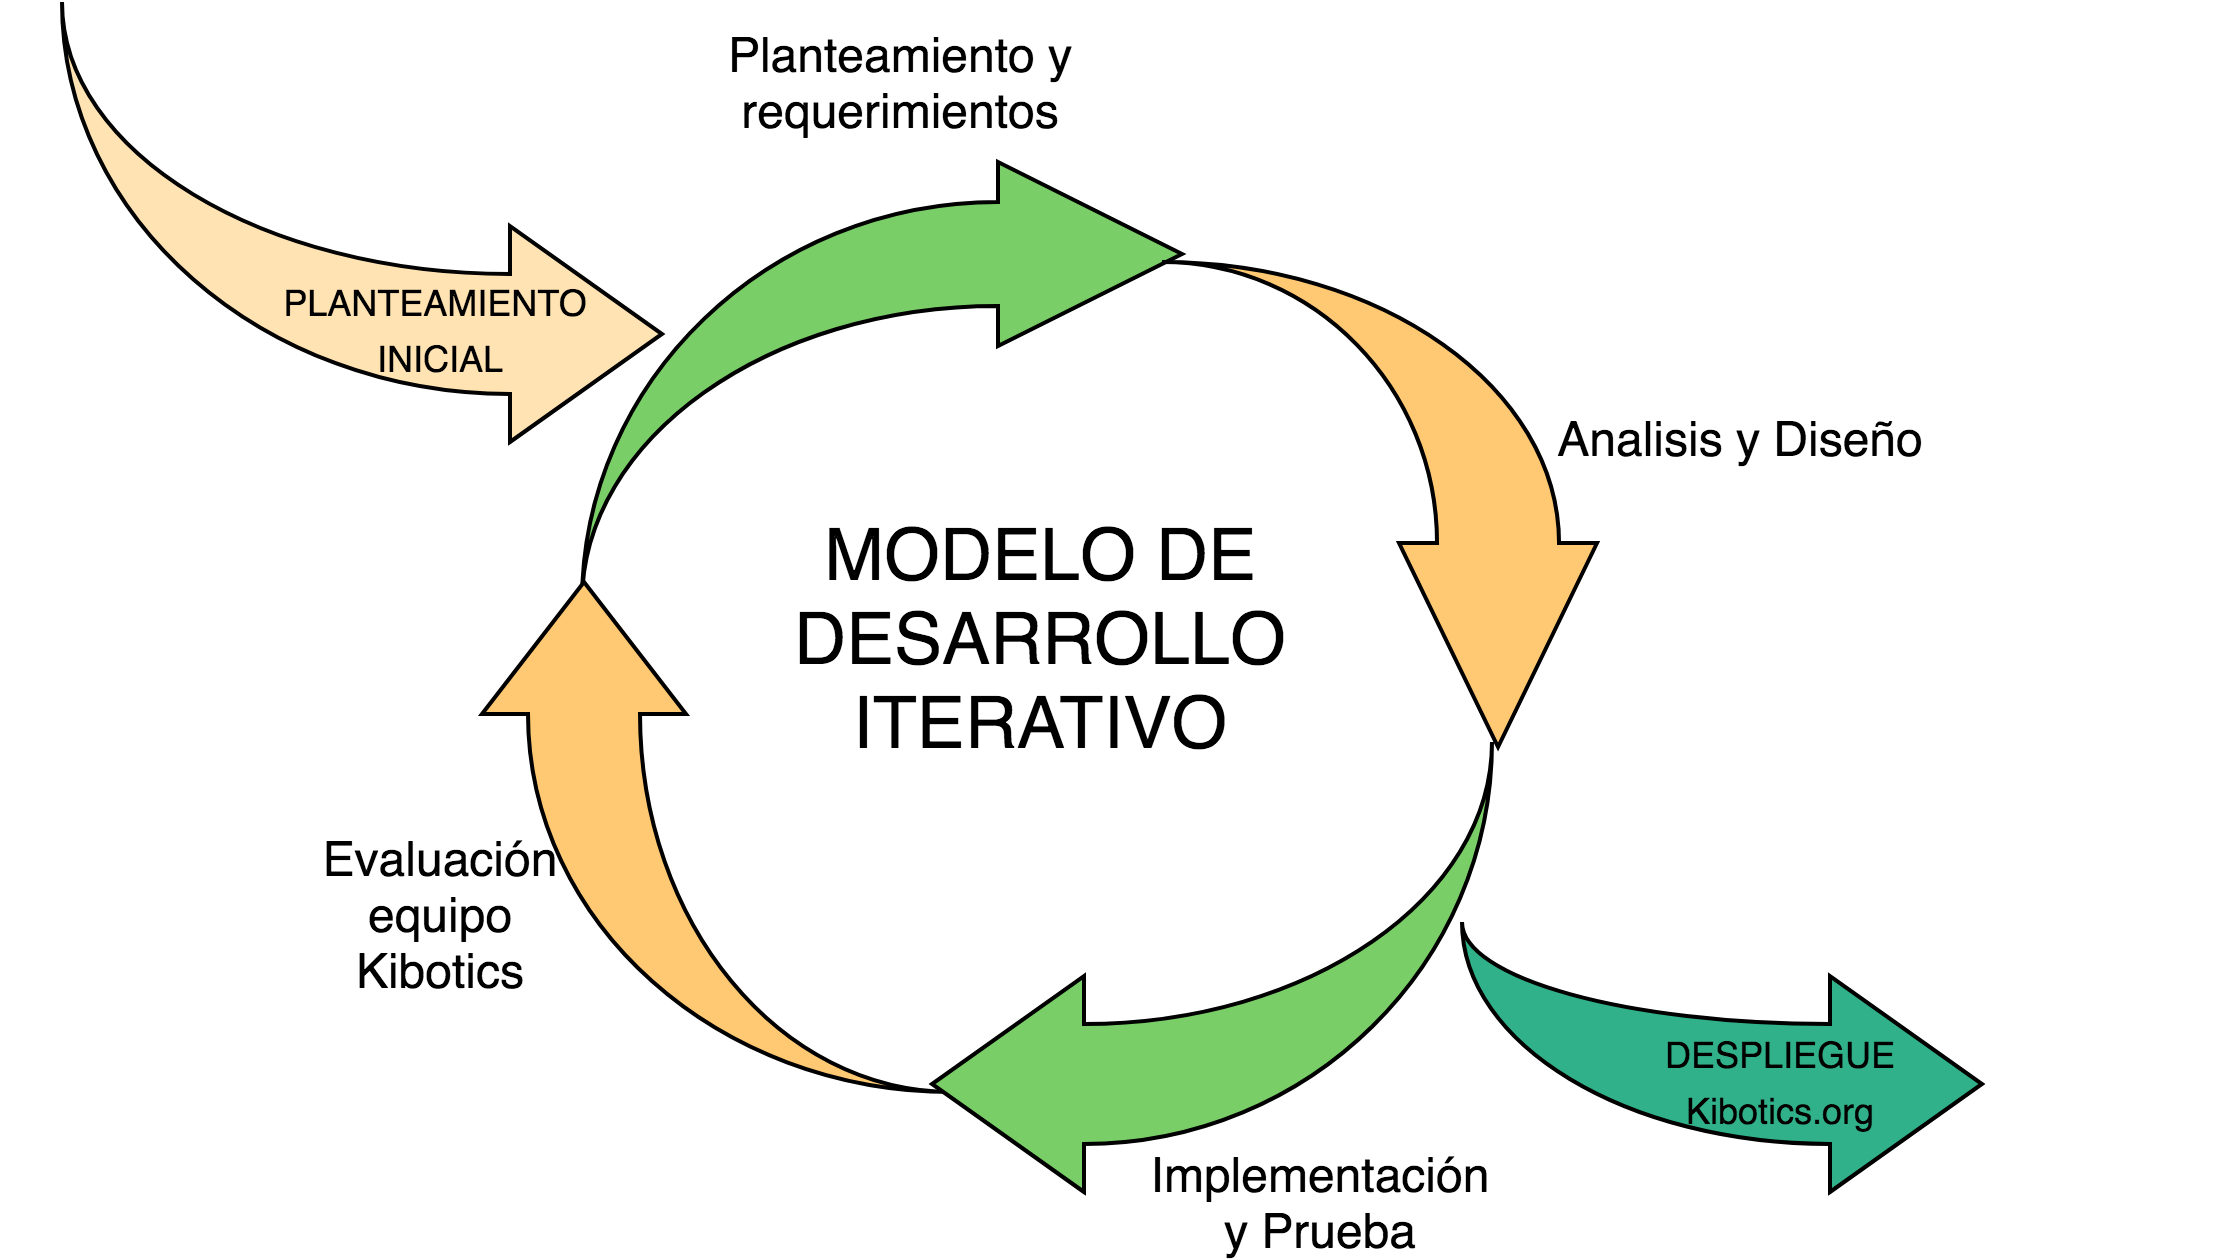
\includegraphics[width=0.6\columnwidth]{chapters/images/metodologiaiterativa.png}
    \caption{Modelo iterativo}
    \label{fig:my_label}
\end{figure}


El código desarrollado y las mejoras se han integrado progresivamente en el código fuente oficial de Kibotics en GitHub \footnote{https://github.com/} mediante su flujo de trabajo  incidencia (\textit{issue}), rama (\textit{branch}) y parche (\textit{pullresquest}). De esta forma la plataforma oficial está siempre actualizada con los últimos cambios añadidos y verificados por el equipo de desarrolladores.

Para llevar acabo esta metodología se establecieron reuniones semanales con el tutor para la orientación de este trabajo fin de grado. A lo largo del proyecto se ha mantenido la comunicación con el tutor y el equipo de Kibotics a través de la plataforma Slack \footnote{https://slack.com/}. 



Además se ha creado una página web tipo blog para llevar un seguimiento de las tareas realizadas y los objetivos semanales. \footnote{https://roboticslaburjc.github.io/2020-tfg-marta-quintana/}

\begin{figure}[H]
    \centering
    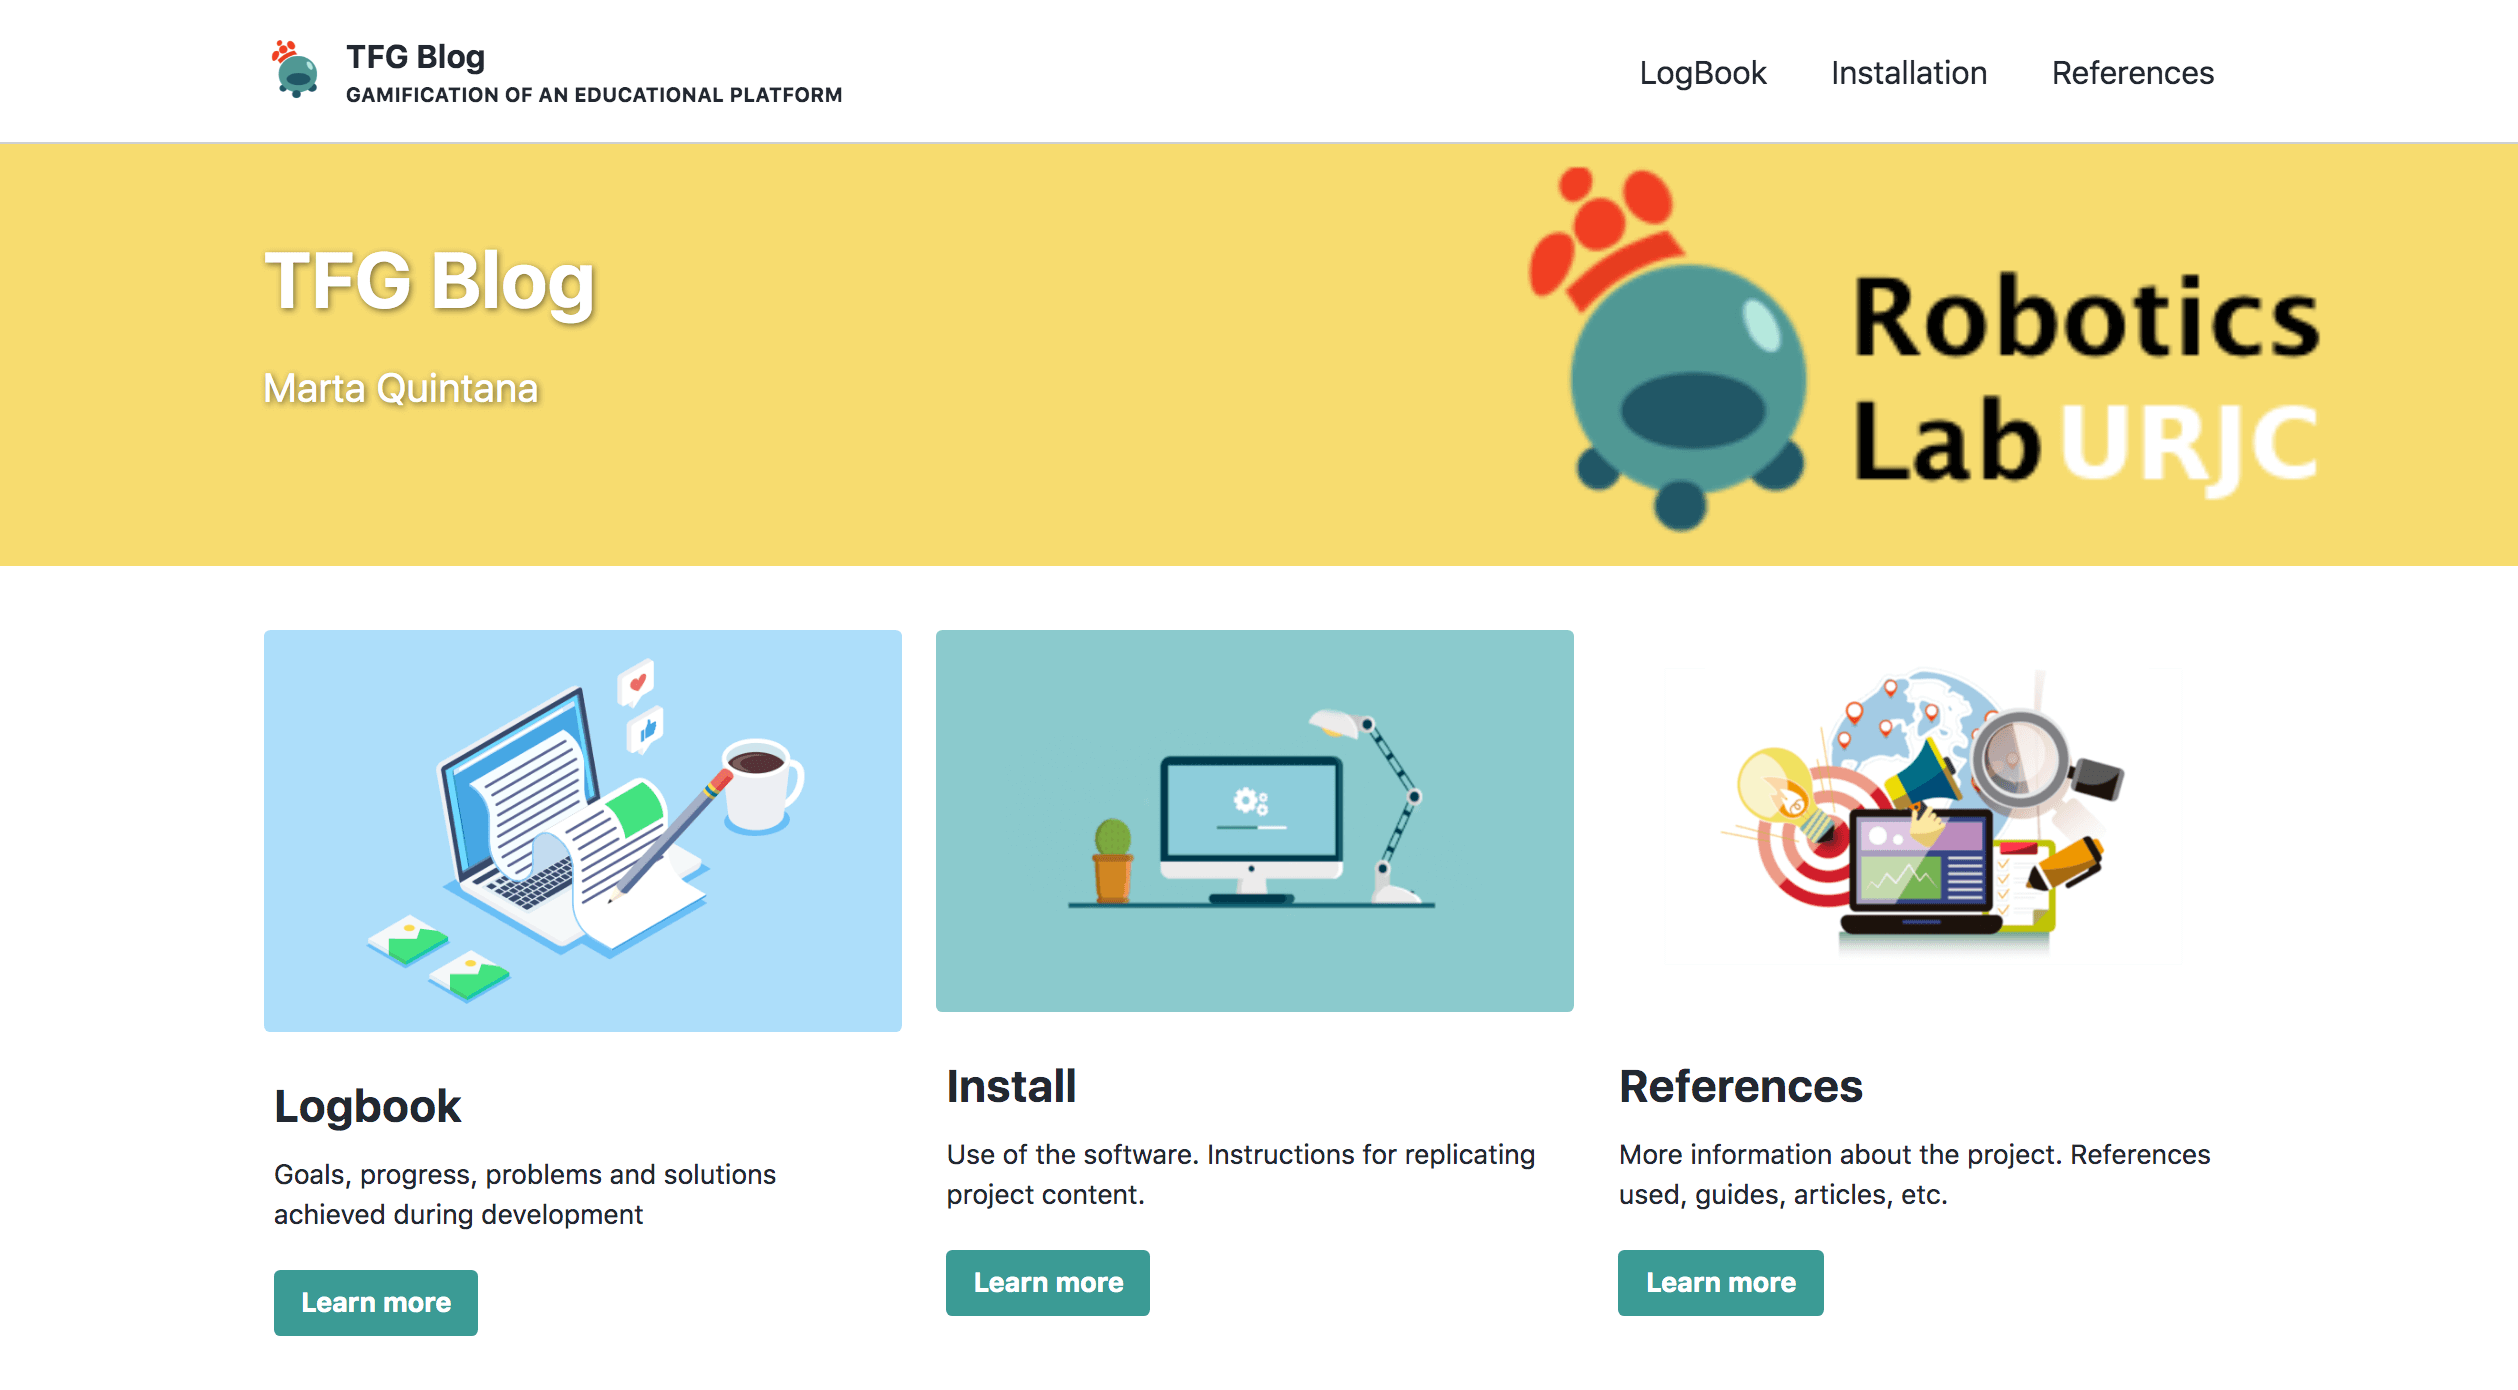
\includegraphics[width=0.6\linewidth]{chapters/images/webtfg.png}
    \caption{Página web de este TFG}
    \label{fig:my_label}
\end{figure}

\section{Plan de Trabajo}
El plan de trabajo seguido durante este proyecto se puede dividir en las siguientes etapas:


\begin{itemize}
    \item \textbf{Aterrizaje en Kibotics y repaso de tecnologías web}: Toma de contacto con Kibotics y repaso de HTML5, JavaScript, Django y otras tecnologías que se utilizan en la plataforma.
    
    \item \textbf{Estudio Web Audio API y Tensor FlowJS}: Realización de ejercicios y tutoriales de distintas herramientas para introducir sonido y reconocimiento de audio en Kibotics.
   
    \item \textbf{Diseño Teleoperador Acústico con Teachable Machine}: Creación de un teleoperador acústico con reconocimiento de audio. 

    \item \textbf{Prototipo de aspiradora robótica}: Diseño y creación de modelos del nuevo ejercicio.
    \item \textbf{Diseño ejercicio aspiradora robótica confeti}: Desarrollo de una aspiradora robótica simulada, un nuevo actuador de absorción y piezas de confeti que puedan ser absorbidas por la aspiradora.
    
    \item \textbf{Prototipo ejercicio Mbot con Pinza basado en A-Frame}: Creación de un prototipo en A-Frame nativo para el estudio de las físicas y mallas de colisión. 
    \item \textbf{Preparación del ejercicio del pañuelo}: Creación e implementación del ejercicio, desarrollo del circuito, una lata y un Mbot con Pinza realizados con Blender y JavaScript, para ofrecernos físicas más realistas.

\end{itemize}



% HERRAMIENTAS %
%%%%%%%%%%%%%%%%%%%%%%%%%%%%%%%%%%%%%%%%%%%%%%%%%%%%%%%%%%%%%%%%%%%%%%%%%%%%%%%%
\chapter{Infraestructura utilizada}
\label{infraestructura}
En este capítulo vamos a profundizar en las tecnologías y herramientas que se han empleado a lo largo de este trabajo. Por un lado se explican los lenguajes de programación (JavaScript, Python y Scratch) y los lenguajes de documentos (HTML5 y JSON)  utilizados. Por otro lado, hablaremos de TensorFlowJS, Web Audio API y Teachable Machine, tecnologías que nos ofrecen procesamiento de audio en aplicaciones web. Otras aplicaciones como Blender y A-Frame han sido fundamentales para el  modelado 3D y realidad virtual. Finalmente, hablaremos de la plataforma Kibotics, su estructura y las tecnologías web que la componen.
\section{Lenguajes de programación y de documentos}
\subsection{HTML5}
HTML5 es la última versión de HTML cuyas siglas corresponden a \textit{``HyperText Markup Language''} es el bloque de construcción más básico de la Web\cite{html}. \textit{``HyperText''} significa hipertexto, se refiere a enlaces que conectan páginas web entre sí, ya sea dentro de un único sitio web o entre sitios web. 
\textit{``Markup''} significa marca o etiqueta, ya que todas las páginas web están construidas en base a etiquetas. Con ellas se anota texto, imágenes y otros contenidos para mostrar en un navegador web. El formato HTML5 incluye etiquetas como:  \textless head\textgreater, \textless title\textgreater, \textless body\textgreater, \textless header\textgreater, \textless footer\textgreater, \textless article\textgreater, \textless section\textgreater, \textless p\textgreater, \textless div\textgreater, \textless span\textgreater, \textless img\textgreater, \textless aside\textgreater, \textless audio\textgreater, \textless canvas\textgreater, \textless datalist\textgreater, \textless details\textgreater, \textless embed\textgreater, \textless nav\textgreater, \textless output\textgreater, \textless progress\textgreater, \textless video\textgreater, \textless ul\textgreater, \textless ol\textgreater, \textless li\textgreater  y otros. En la Figura 3.1(a) podemos ver cómo es el uso de las etiquetas para la creación de una página web y en la Figura 3.1(b) cómo se visualizaría en el navegador.

Hablamos de \textit{``Language''} porque HTML es un lenguaje, tiene sus normas, tiene su estructura y una serie de convenciones que nos sirven para definir tanto la estructura como el contenido de una web. Esto no quiere decir que sea un lenguaje de programación. HTML no tiene estructuras de lenguaje de programación, como los bucles, las condiciones, las funciones, etcétera. HTML5 es un estándar que sirve para definir la estructura y el contenido de una página Web \cite{html2}. 

\begin{figure}[H]
    \begin{subfigure}[b]{0.5\textwidth}
  \centering
    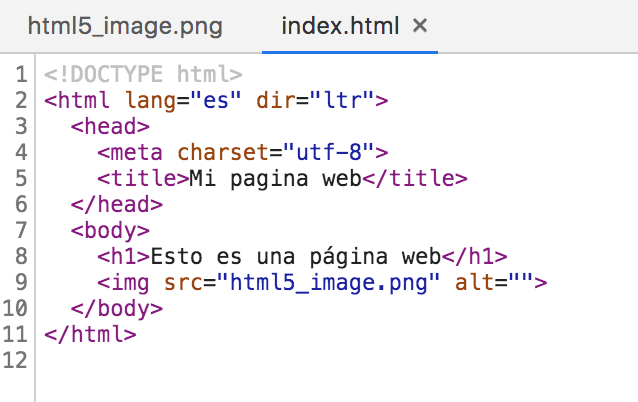
\includegraphics[width=0.9\textwidth, height=0.5\textwidth]{chapters/images/simplehtmlpage.png}
    \caption{Fuente de la página web}
    \label{fig:f2}
  \end{subfigure}
  \begin{subfigure}[b]{0.5\textwidth}
  \centering
    
\includegraphics[width=0.9\textwidth, height=0.5\textwidth]{chapters/images/simplehtml.png}
    \caption{Página web visualización}
    \label{fig:f1}
  \end{subfigure}
  \hfill
  
  \caption{Ejemplo de página web con HTML5}
\end{figure}

Generalmente junto con HTML se utilizan otras dos tecnologías web: CSS para la apariencia/presentación y JavaScript para la funcionalidad/comportamiento de una página web.
\\
\\
Kibotics utiliza plantillas basadas en HTML5 en las páginas web que sirve. En este TFG se va a utilizar HTML5 para modificar y crear las plantillas de las páginas web que mostrarán los nuevos ejercicios que vamos a introducir en la plataforma.

\subsection{JavaScript}
JavaScript es un lenguaje de programación interpretado, no necesita compilar los programas para ejecutarlos, pero sí un intérprete que en nuestro caso es el navegador. JavaScript sigue el estándar ECMAScript que se encarga de regir cómo debe ser interpretado, su operatividad y buen funcionamiento. Este lenguaje posee una sintaxis derivada de C y Java pero no tiene nada que ver con ellos.

Se utiliza principalmente para crear páginas web interactivas, que incorporan efectos como texto que aparece y
desaparece, animaciones, acciones que se activan al pulsar botones y ventanas con
mensajes de aviso al usuario\cite{javascript}.

El código JavaScript se ejecuta en el navegador del cliente y permite que éste interactúe con la página web. En la siguiente Figura 3.2 podemos ver un ejemplo de página web interactiva.\footnote{https://martaquintana.github.io/2018-19-CSAAI-Pong/pong-01.html}

\begin{figure}[H]
  \begin{subfigure}[b]{0.5\textwidth}
  \centering
    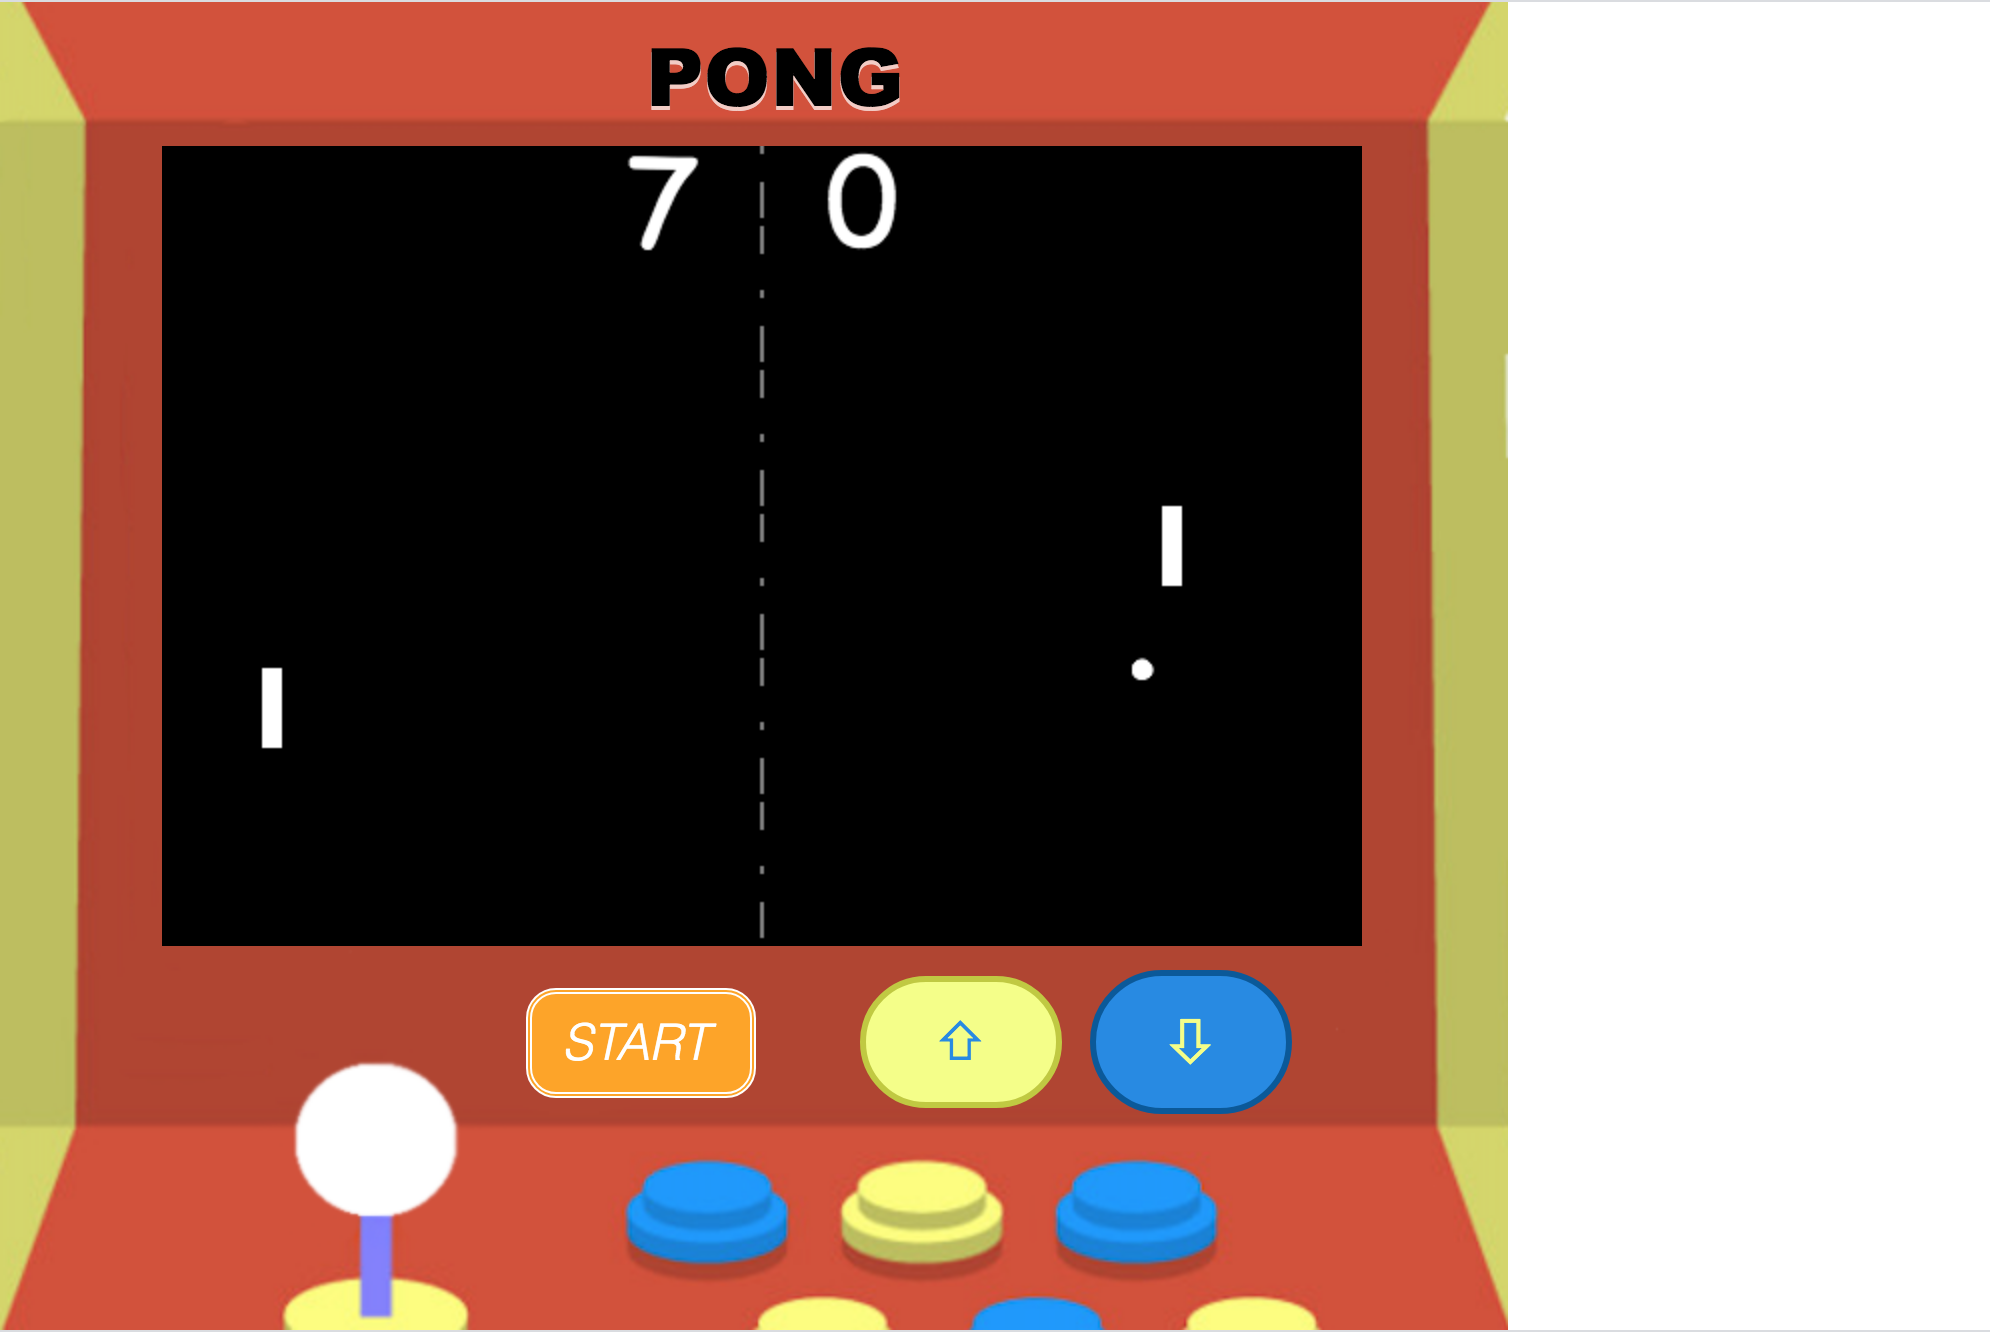
\includegraphics[width=1\textwidth, height=0.6\textwidth]{chapters/images/pong.png}
    \caption{Página web visualización}
    \label{fig:f1}
  \end{subfigure}
  \hfill
  \begin{subfigure}[b]{0.5\textwidth}
  \centering
    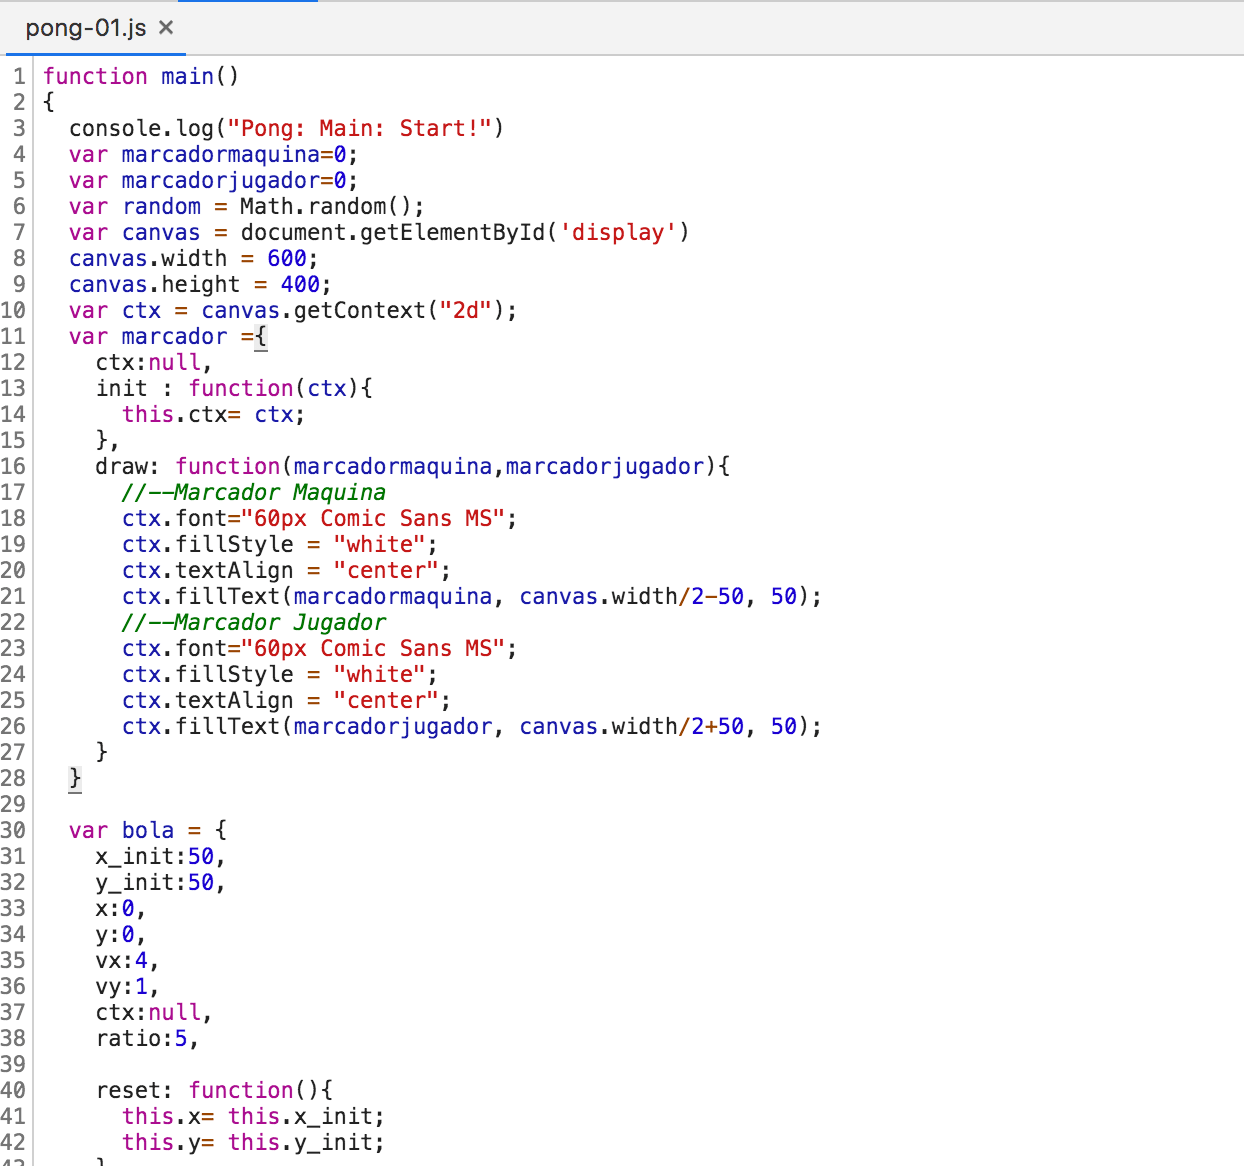
\includegraphics[width=1\textwidth, height=0.6\textwidth]{chapters/images/codigojs.png}
    \caption{Código JavaScript}
    \label{fig:f2}
  \end{subfigure}
  \caption{Ejemplo de página web interactiva con HTML5, CSS3 y JavaScript }
\end{figure}

En este trabajo JavaScript ha sido una pieza clave para su desarrollo y todos los ejercicios se han creado usando este lenguaje de programación.
 
\subsection{Python y Scratch}

Python es un lenguaje de programación orientado a objetos, es un lenguaje interpretado o de script, y al igual que JavaScript necesita un programa intermedio que haga de ``intérprete''. Es un lenguaje fuertemente tipado y multiplataforma. Su filosofía es que el código sea legible y tenga  una sintaxis muy limpia. Sencillo pero potente, lenguaje muy usado en la universidad y trabajo \cite{python}.

El servidor de Kibotics está programado en Python (usa la tecnología web Django). Los ejercicios disponibles en la plataforma se pueden resolver también con este lenguaje. Para usar Python las páginas web de los ejercicios contienen el editor ACE. ACE es un editor de código incrustable escrito en JavaScript \cite{aceeditor}. Esto permite al usuario escribir el código de la solución del ejercicio en Python e internamente este código se traduce a JavaScript para el correcto funcionamiento de los ejercicios. 

Como hemos comentado en la introducción, Scratch es un lenguaje de programación visual basado en bloques, creado y mantenido por Lifelong Kindergarten group en el MIT Media Lab. Para usar Scratch en Kibotics se usa Blocky, que es una librería de JavaScript desarrollada por Google. Permite usar en una página web un editor de código visual. Es compatible con Chrome, Firefox, Safari, Opera y otros navegadores. Corresponde a tecnologías del lado cliente y no tiene dependencia con el servidor \cite{blocky}.


Los ejercicios planteados en este TFG están resueltos tanto en Python como en Scratch. Al ser una plataforma para el ámbito educativo estos dos lenguajes son una buena alternativa para empezar a programar porque son lenguajes sencillos y con una curva de aprendizaje muy suave. En la Figura 3.3 podemos ver unos ejemplos de soluciones.

\begin{figure}[H]
  \begin{subfigure}[b]{1\textwidth}
  \centering
    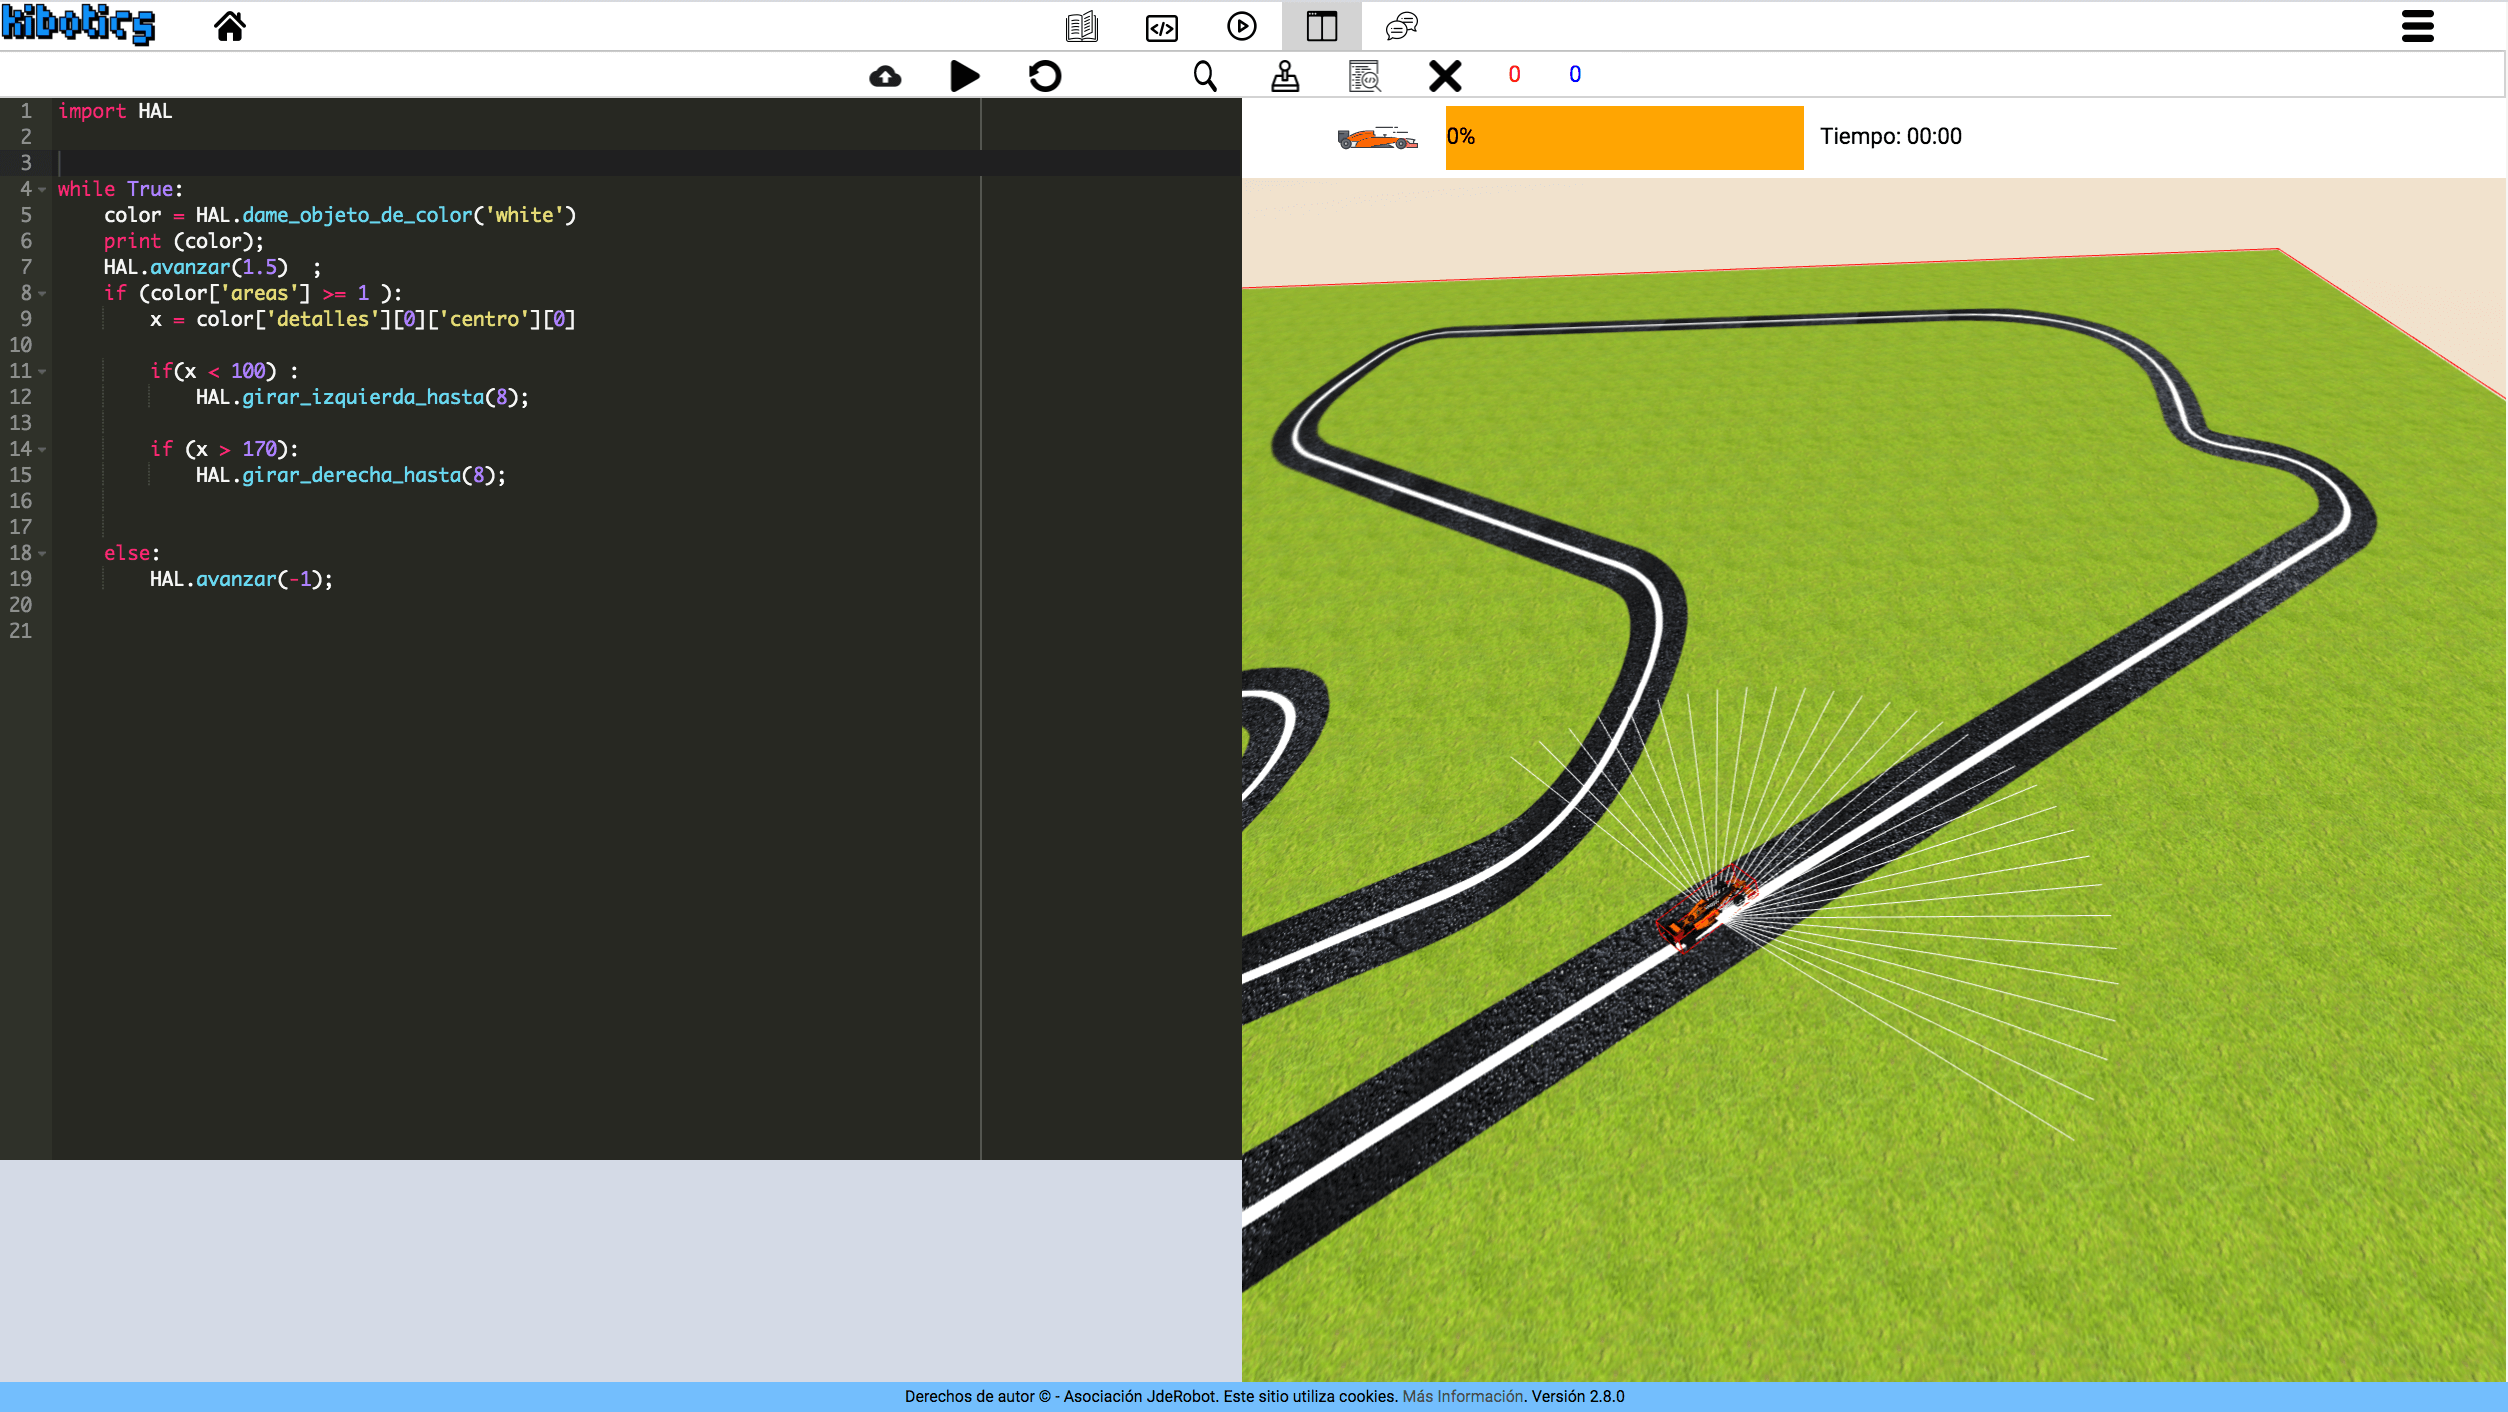
\includegraphics[width=0.95\textwidth, height=0.4\textwidth]{chapters/images/python.png}
    \caption{Solución en Python}
    \label{fig:f1}
  \end{subfigure}
  \hfill
  \begin{subfigure}[b]{1\textwidth}
  \centering
    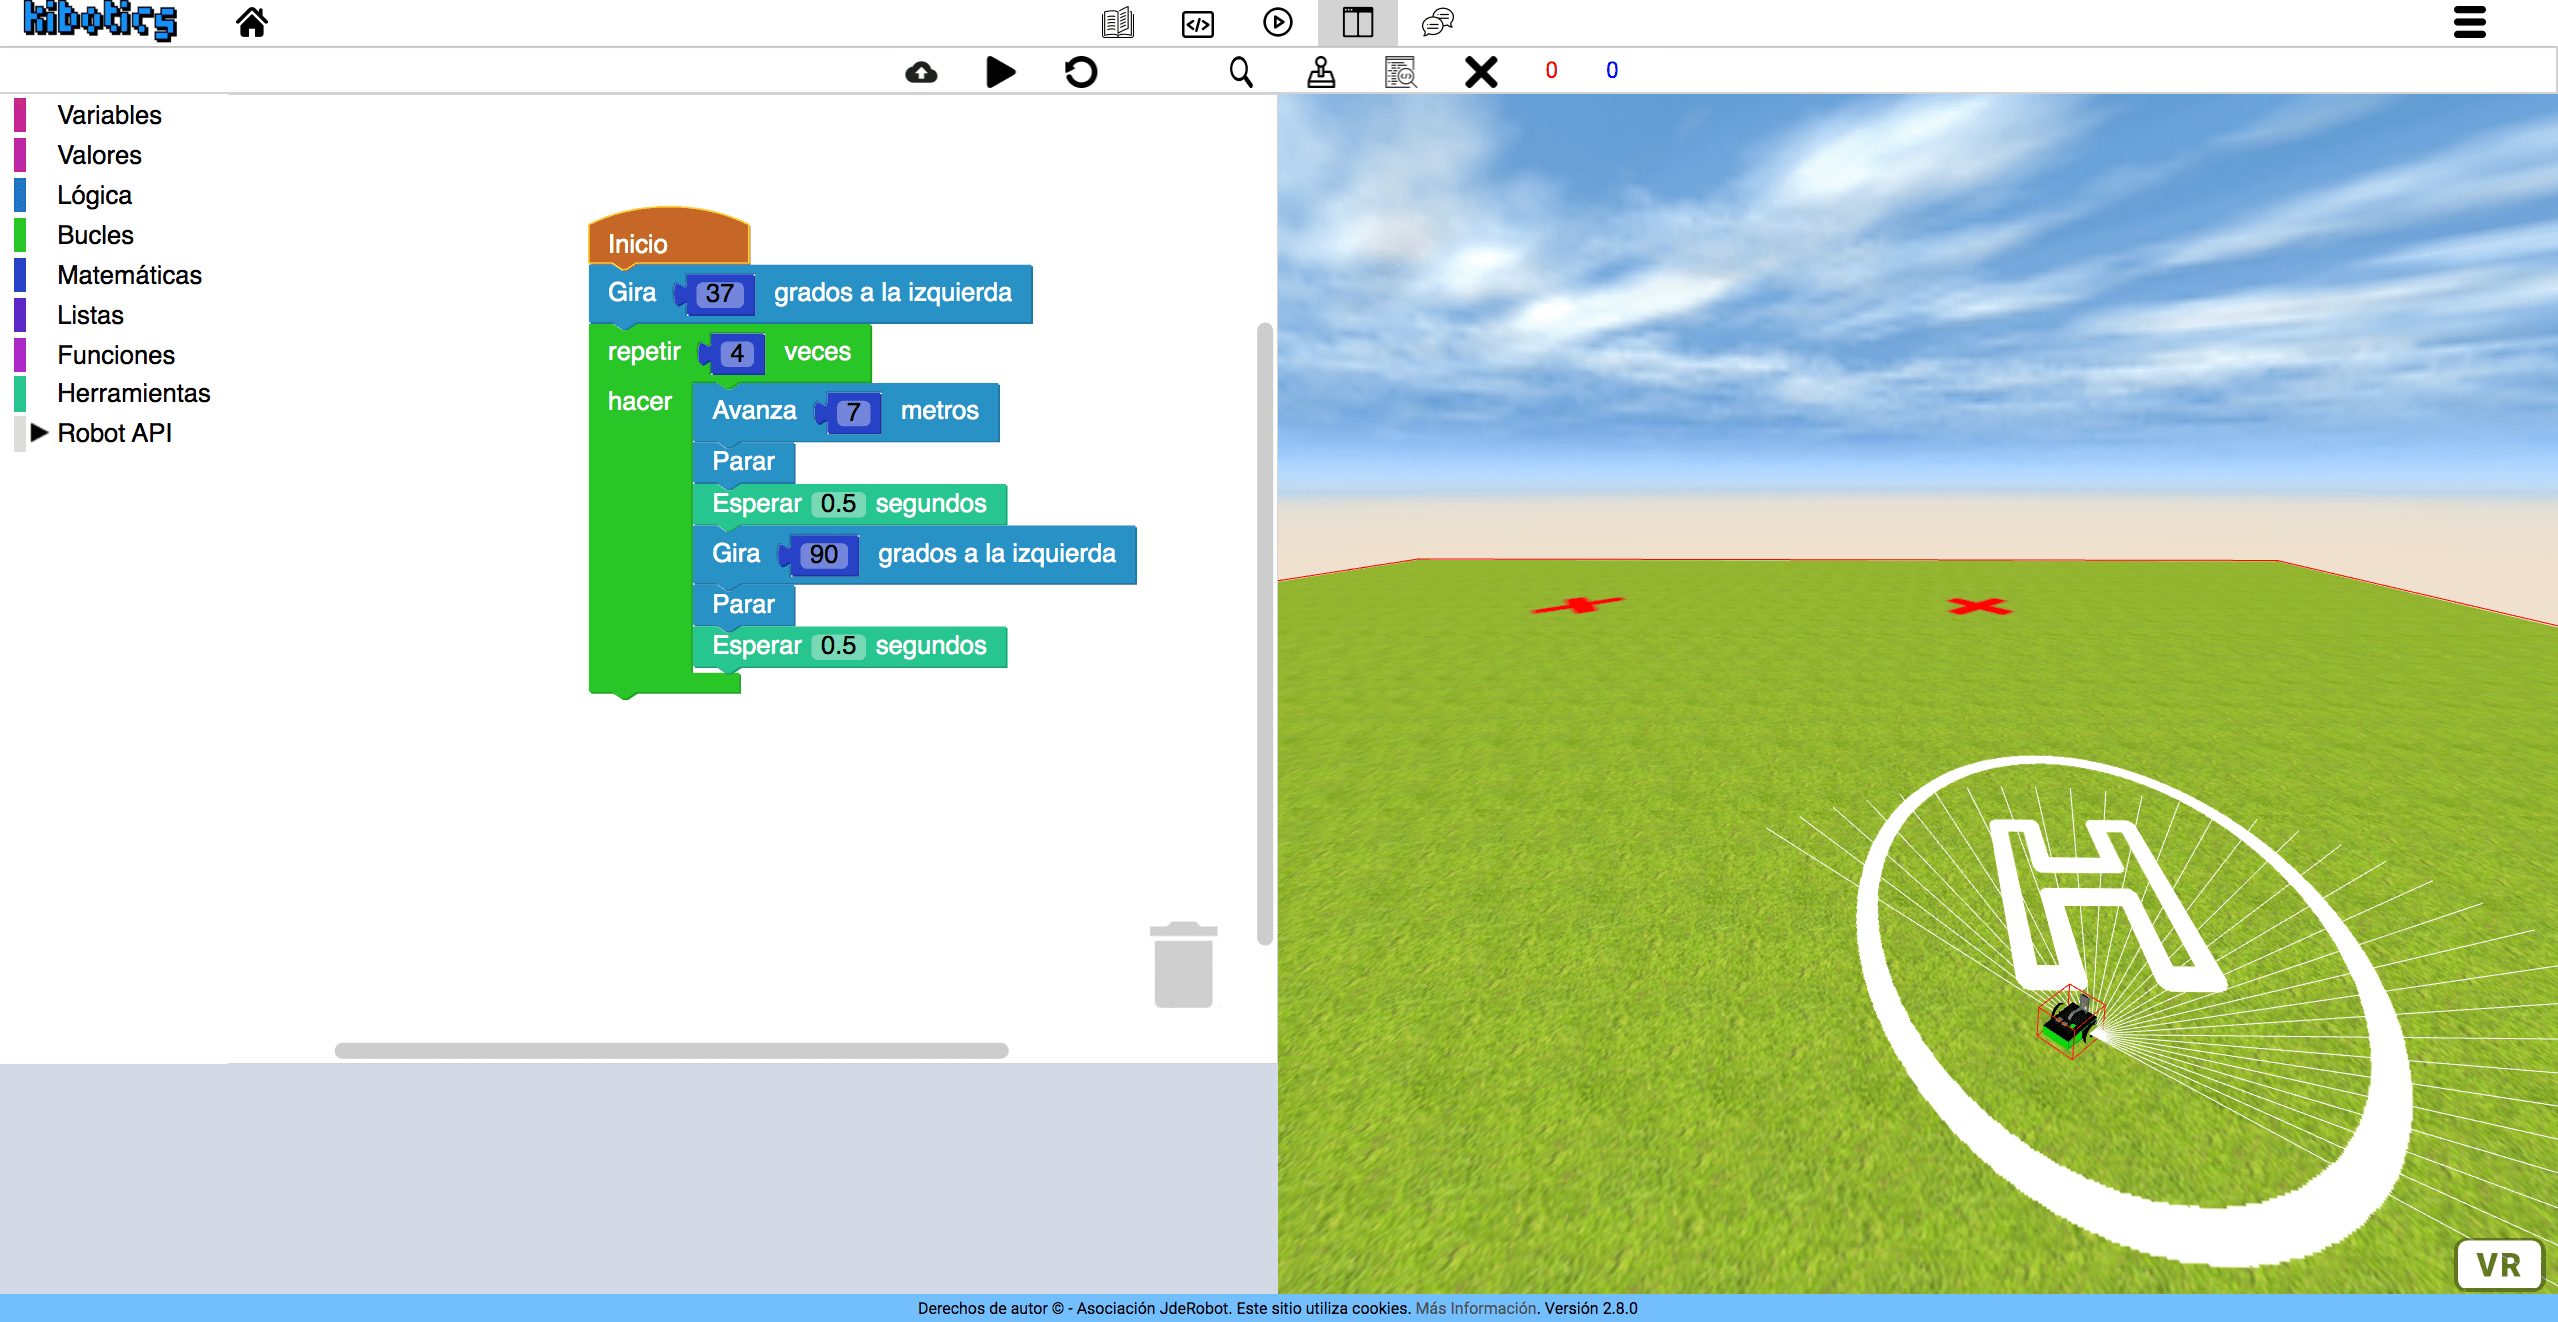
\includegraphics[width=0.95\textwidth, height=0.4\textwidth]{chapters/images/scratch2.png}
    \caption{Solución en Scratch}
    \label{fig:f2}
  \end{subfigure}
  \caption{Ejemplo de código en Kibotics }
\end{figure}


\subsection{JSON} JSON, cuyas siglas significan JavaScript Object Notation, es un formato de intercambio de datos muy ligero. Para nosotros es fácil de leer y escribir, además la interpretación y generación de ficheros es muy sencilla para las máquinas \cite{json}.

JSON es un formato de datos basado en texto estándar para representar datos estructurados con la sintaxis de objetos de JavaScript. Son archivos de texto plano con codificación UTF8, que son compatibles con todos los sistemas. Se utiliza para transmitir datos en aplicaciones web \cite{json2}. 
Este formato puede ser utilizado independientemente de JavaScript, y muchos entornos de programación poseen la capacidad de leer (convertir; \textit{parsear}) y generar ficheros JSON. En nuestro caso vamos a leer ficheros JSON desde JavaScript.

Un fichero JSON  típicamente está compuesto de dos estructuras: 
\begin{itemize}
    \item \textbf{Una colección de pares de nombre/valor}: En otros lenguajes son conocidos como objeto, registro, estructura, diccionario o lista de claves. 
    Ejemplo objeto: 
    \begin{lstlisting}
    {
        "id" : 7,
        "name" : "Robot",
        "type" : "Drone"
    }
     \end{lstlisting}
    \item \textbf{Una lista ordenada de valores}: En la mayoría de los lenguajes, esto se implementa como arreglos \textit{arrays}, vectores o listas.  
     Ejemplo array:  
     \begin{lstlisting}
        [ "blue", "yellow", "orange" ]
     \end{lstlisting}
\end{itemize}

Estas estructuras son universales en todos los lenguajes de programación, es por esto que  JSON es muy fácil utilizar para un programador. Todos los lenguajes disponen de funciones para interpretar cadenas JSON y convertir datos en cadenas JSON válidas.

En la Figura 3.4 podemos ver una pequeña parte de un fichero de configuración de un ejercicio con JSON en Kibotics. En esta plataforma se utiliza JSON para crear los ejercicios con las características específicas que le correspondan y en este TFG se han usado tanto para la creación de los mundos como para fijar las posiciones de los confetis en el ejercicio del Roomba que veremos más adelante.

\begin{figure}[H]
    \centering
    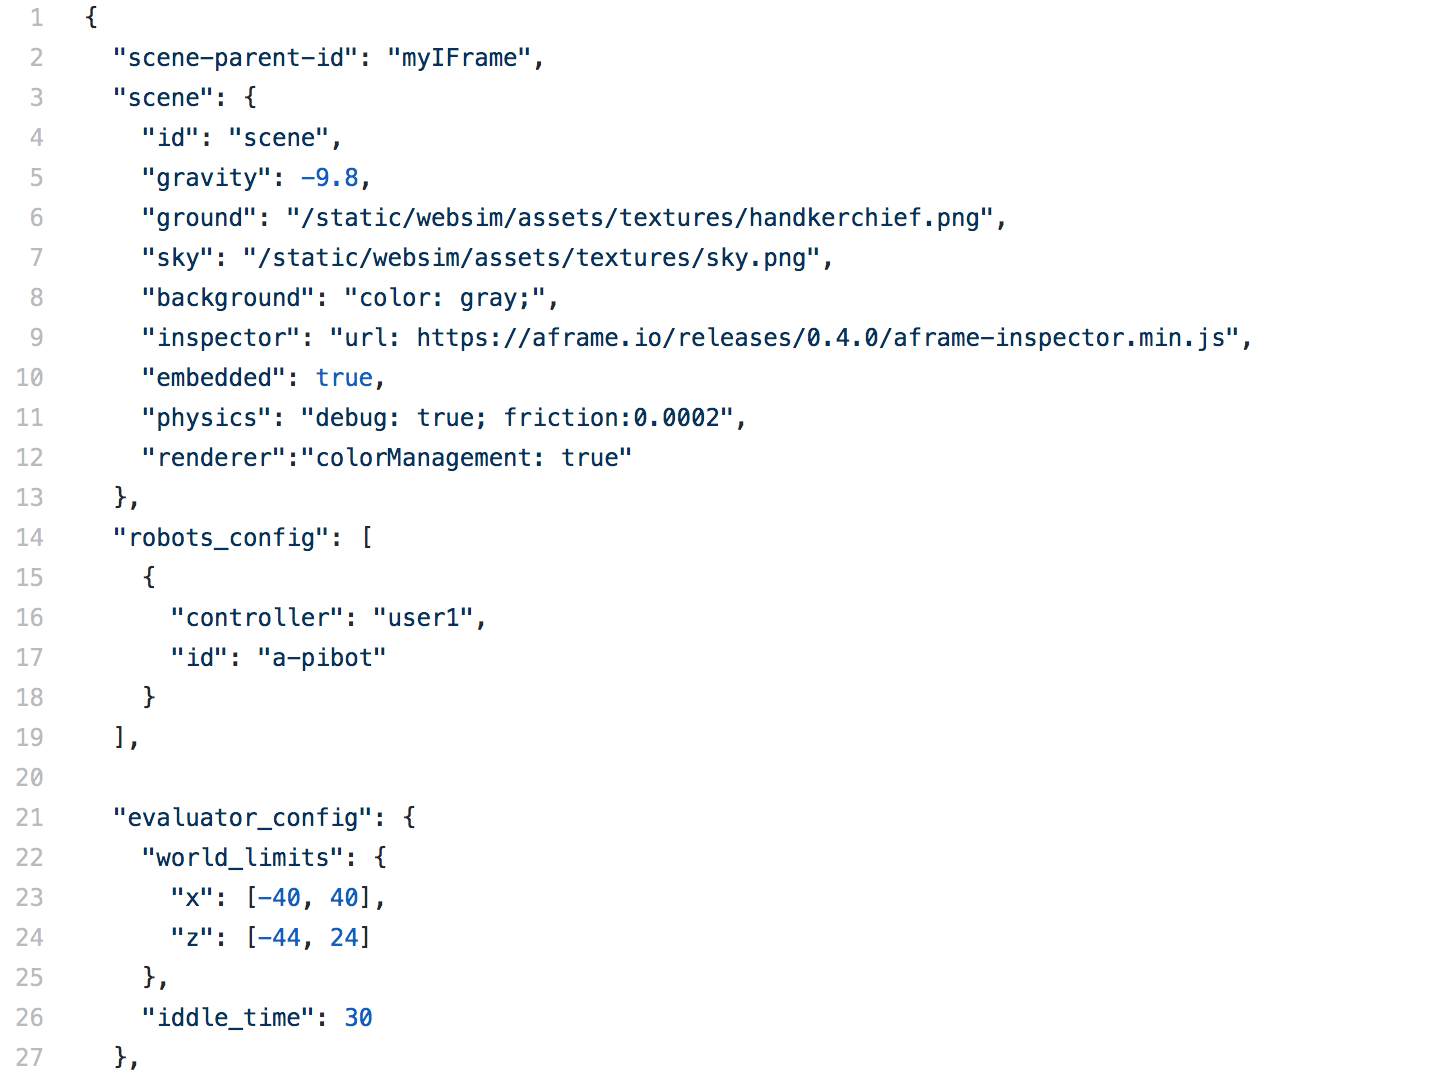
\includegraphics[width=0.6\textwidth, height=0.4\textwidth]{chapters/images/json.png}
    \caption{Parte de un fichero config.json de un ejercicio en Kibotics}
    \label{fig:my_label}
\end{figure}

\section{Herramientas}
\subsection{TensorFlowJS, Web Audio API y Teachable Machine}
Para procesar el audio en JavaScript se han tenido que analizar diferentes herramientas o APIs\footnote{Interfaz de programación de aplicaciones} de procesamiento de audio en la web. De esta forma hemos podido elegir la herramienta que mejor se adapta a nuestro problema.
Entre ellas TensorFlowJS, Web Audio API y Teachable Machine (Figura 3.5) son las herramientas que se han estudiado para llevar a cabo el teleoperador acústico.
\\
TensorFlowJS es una biblioteca de JavaScript para el entrenamiento y la implementación de modelos de aprendizaje automático en navegadores y en Node.js . TensorFlow es una plataforma de código abierto para la creación de modelos de aprendizaje automático \cite{tfjs}.

La API de Audio Web provee un sistema poderoso y versatil para controlar audio en la Web, permitiendo a los desarrolladores escoger fuentes de audio, agregar efectos al audio, crear visualizaciones de audios y aplicar efectos espaciales, entre otras cosas \cite{waa}.

Teachable Machine es una herramienta basada en la Web que hace posible crear modelos de aprendizaje automático de manera rápida, sencilla y accesible para todos \cite{tm}.

\begin{figure}[H]
    \centering
    \begin{subfigure}{.3\linewidth}
        
\includegraphics[width=1\textwidth]{chapters/images/tfjs.png}
        \caption{Tensor Flow JS}
    \end{subfigure}
    \hskip2em
    \begin{subfigure}{.3\linewidth}
    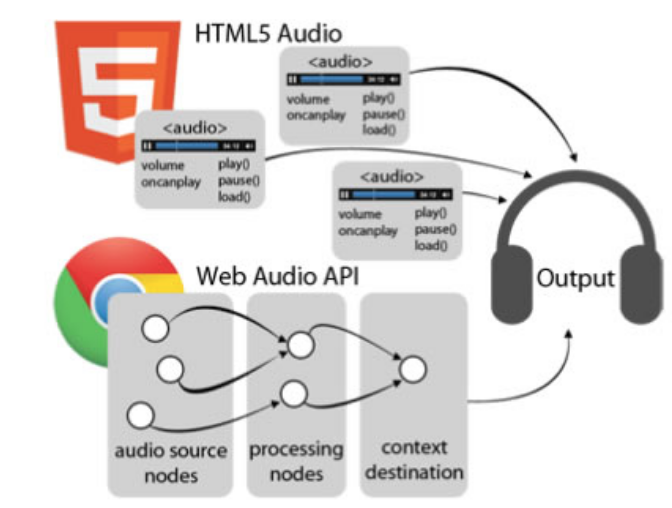
\includegraphics[width=1\textwidth]{chapters/images/waa.png}
        \caption{Web Audio API}
    \end{subfigure}
    \begin{subfigure}{.3\linewidth}
       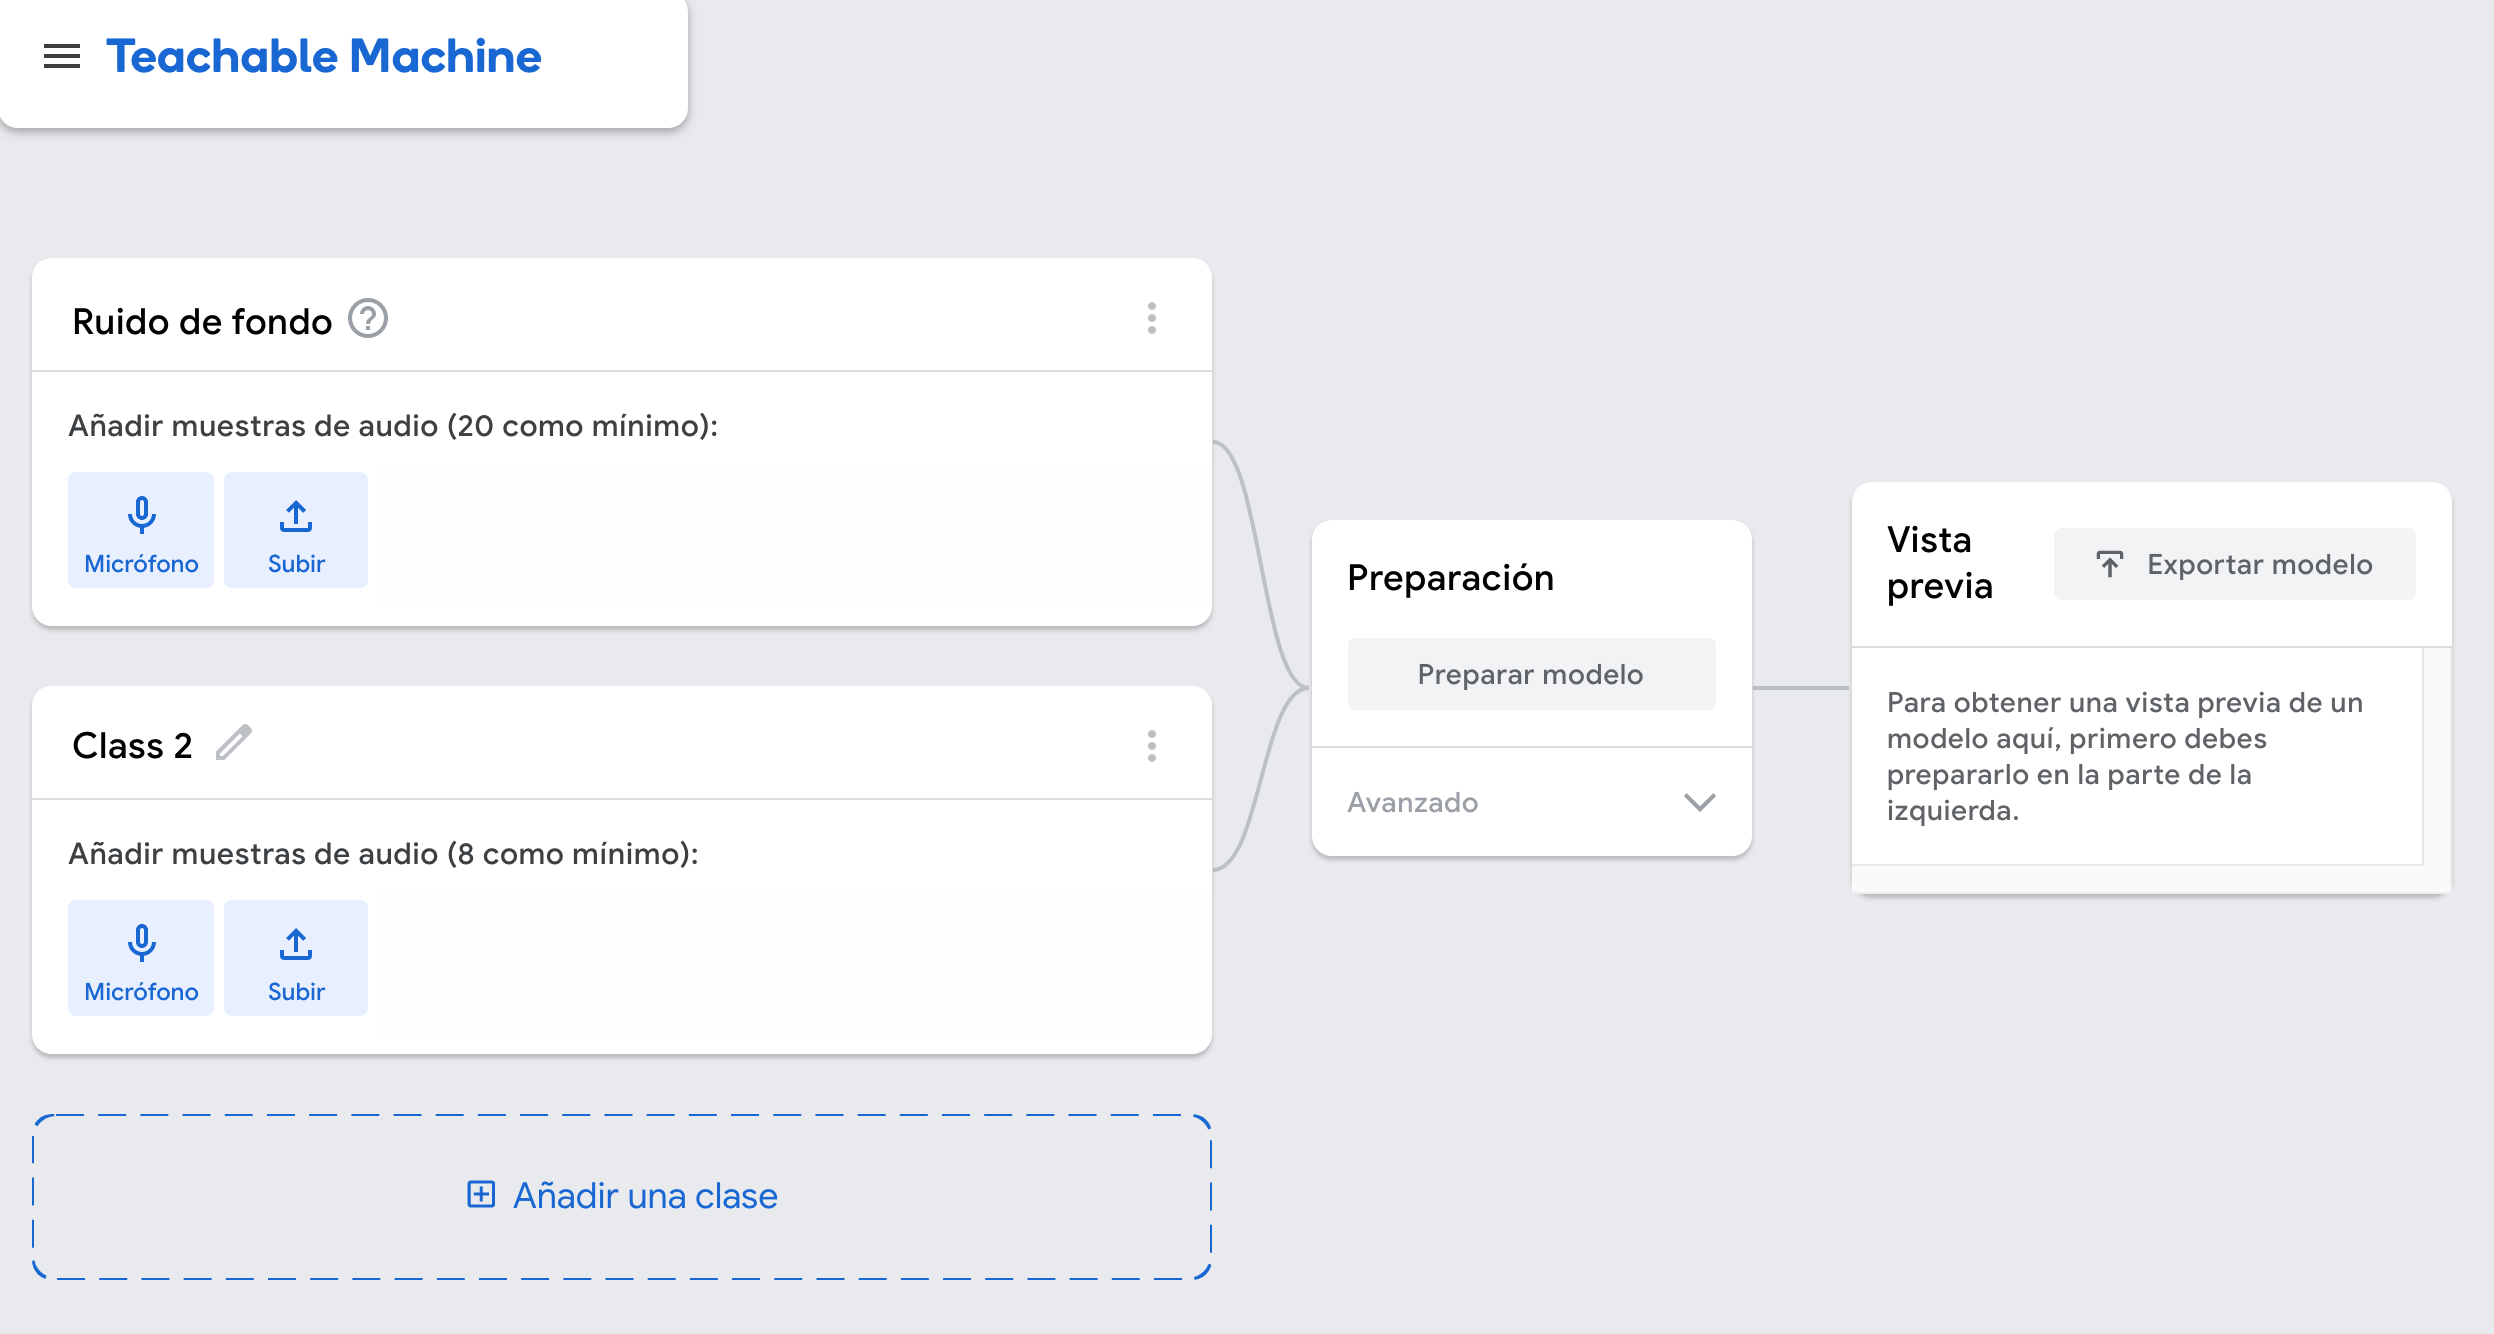
\includegraphics[width=1\textwidth, height=0.7\textwidth]{chapters/images/tm.png}
        \caption{Teachable Machine}
    \end{subfigure}
    \caption{Herramientas de reconocimiento de audio}
\end{figure}


En el Capítulo 4 se explicará en profundidad cómo se han usado estas tecnologías y por qué después de probar con cada una de estas tres herramientas, hemos elegido Teachable Machine para el desarrollo final del Teleoperador Acústico.


\subsection{A-Frame}

A-Frame es un marco web para crear experiencias de realidad virtual (VR). A-Frame utiliza HTML declarativo, lo que facilita bastante la creación de escenas en 3D y es accesible para todos, desde desarrolladores web, artistas y diseñadores, a educadores y estudiantes. Su estructura entidad-componente proporciona una infinidad de posibilidades y ofrece compatibilidad con \textit{three.js}, una biblioteca  escrita en JavaScript para crear y mostrar gráficos animados 3D en un navegador Web. 

Sin instalar nada, A-Frame permite manejar modelos 3D para crear entornos de realidad virtual solamente usando las etiquetas \textless script\textgreater  y \textless a-scene\textgreater. Es compatible con aplicaciones de realidad virtual como GearVR y Windows Mixed Reality entre otras. Además funciona perfectamente en ordenadores y teléfonos inteligentes \cite{aframe}. 


Para crear escenas en una página web solo es necesario importar la librería de A-Frame de esta forma: \begin{lstlisting}
    <script src="https://aframe.io/releases/1.2.0/aframe.min.js"></script>
\end{lstlisting} 
y poner las etiquetas corresponientes a-scene y los objetos que queramos que aparezacan en la escena con sus atributos.
A continuación se muestra un ejemplo de código correspondiente con la visualización de la escena en el navegador en la Figura 3.6.
\\
\begin{lstlisting}
    <html>
      <head>
        <script src="https://aframe.io/releases/1.2.0/aframe.min.js"></script>
      </head>
      <body>
        <a-scene>
          <a-box position="-1 0.5 -3" rotation="0 45 0" color="#4CC3D9"></a-box>
          <a-sphere position="0 1.25 -5" radius="1.25" color="#EF2D5E"></a-sphere>
          <a-cylinder position="1 0.75 -3" radius="0.5" height="1.5" color="#FFC65D"></a-cylinder>
          <a-plane position="0 0 -4" rotation="-90 0 0" width="4" height="4" color="#7BC8A4"></a-plane>
          <a-sky color="#ECECEC"></a-sky>
        </a-scene>
      </body>
    </html>
\end{lstlisting}

\begin{figure}[H]
    \centering
    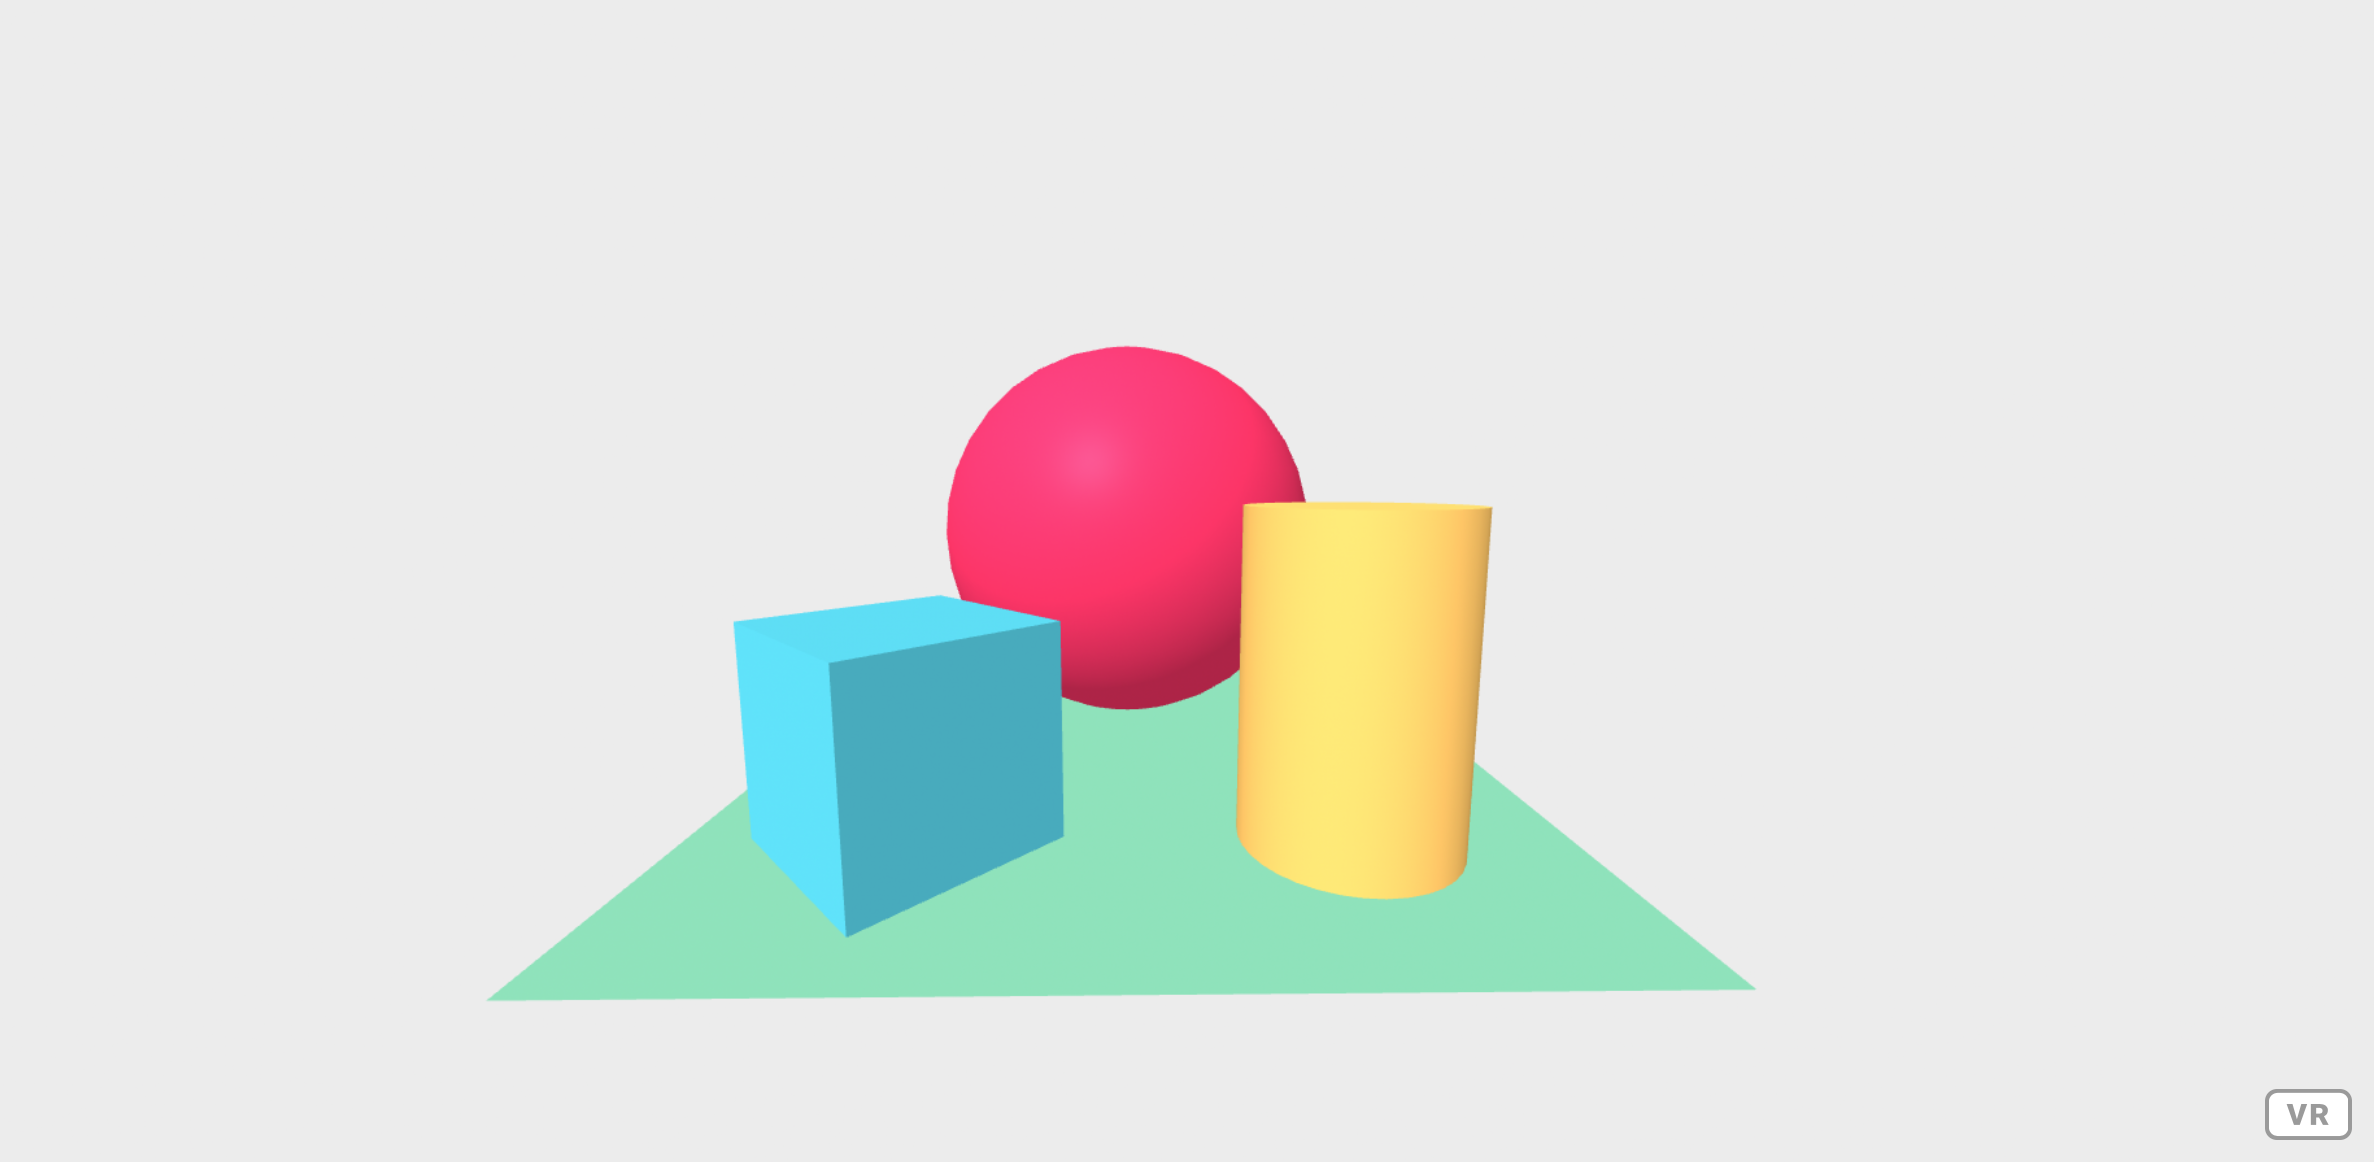
\includegraphics[width=1\textwidth, height=0.5\textwidth]{chapters/images/aframe.png}
    \caption{Ejemplo escena en A-Frame}
    \label{fig:my_label}
\end{figure}

A-Frame proporciona un inspector visual 3D incorporado (Figura 3.7). Presionando ctrl + alt + i, podemos inspeccionar la escena, esto es muy útil cuando necesitas la posición concreta de un objeto.

\begin{figure}[H]
    \centering
    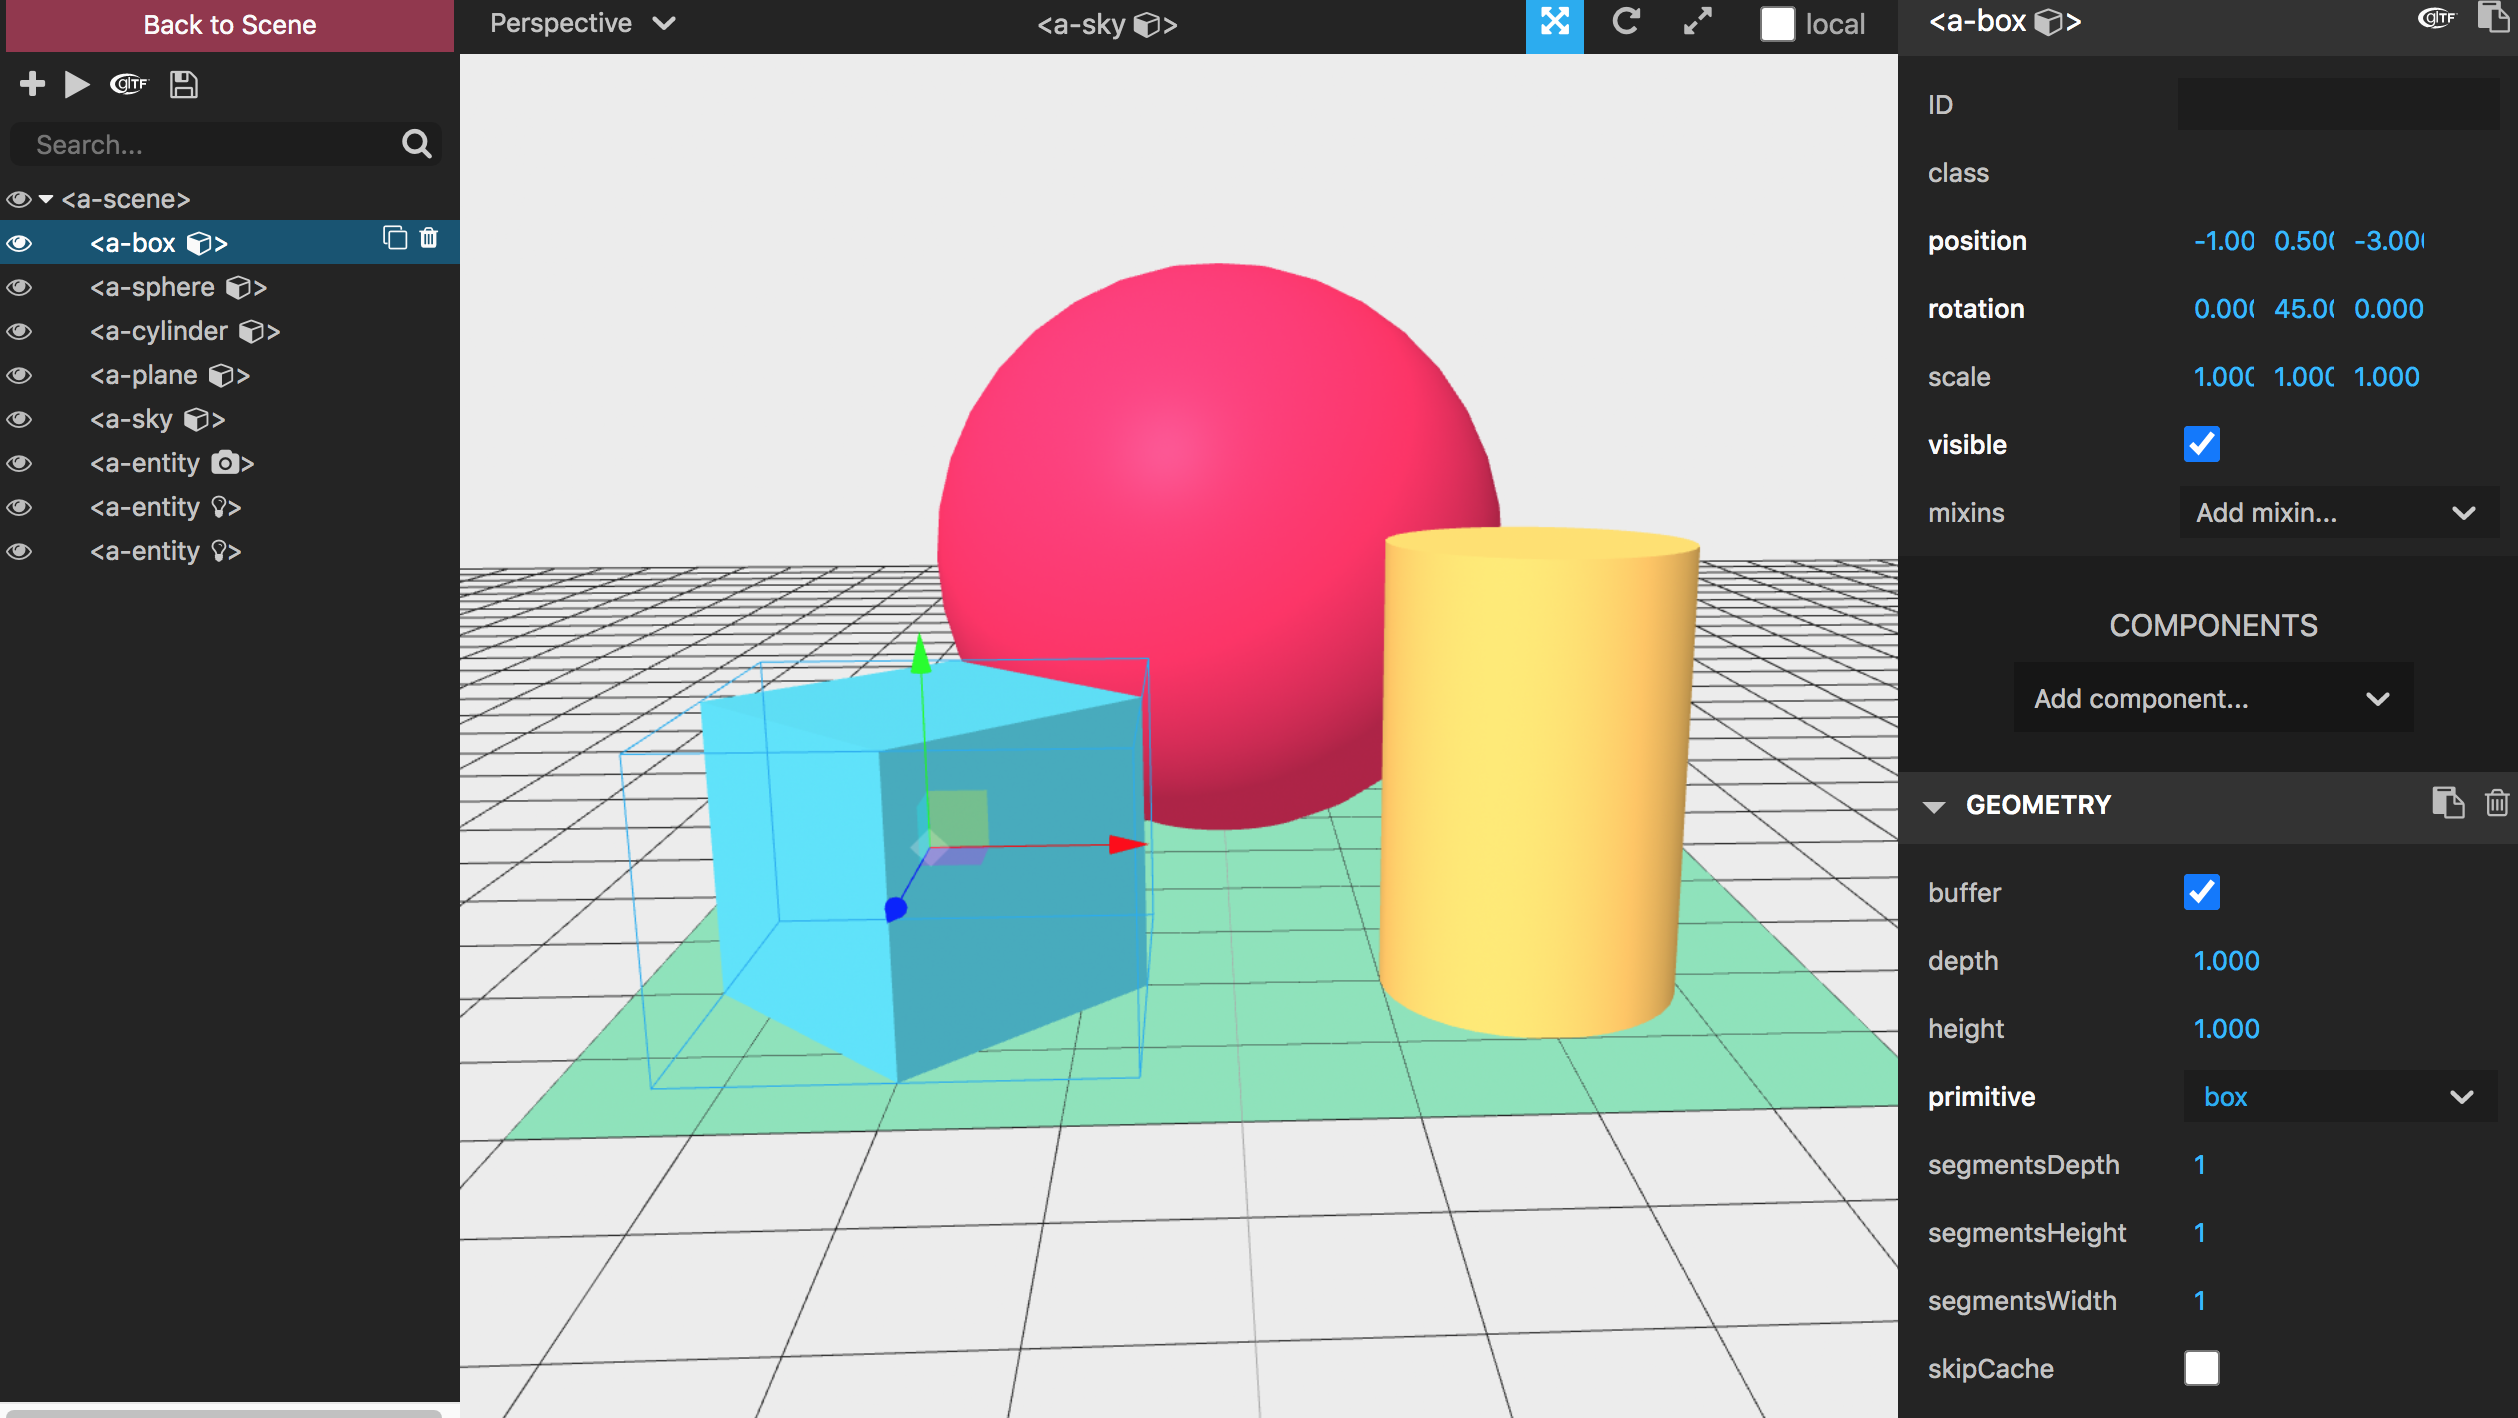
\includegraphics[width=0.8\textwidth, height=0.5\textwidth]{chapters/images/inspectoraframe.png}
    \caption{Inspector en A-Frame}
    \label{fig:my_label}
\end{figure}


En nuestro caso \textit{a-entity} serán los modelos 3D de los robots que se crearán con Blender  y se usarán componentes como \textit{a-box}, \textit{a-plane}, \textit{a-cylinder} y \textit{a-sphere} para crear componentes adicionales a la escena dándoles sus respectivas texturas. En este trabajo se ha usado la versión 1.1.0 de A-Frame.

\subsection{Blender}
Blender es un software de creación de modelos 3D gratuito, de código abierto y multiplataforma. Este programa se utiliza para el modelado, montaje, animación, simulación, renderizado 3d, así como para la  composición y seguimiento de movimiento, edición de vídeo y animación 2D
\cite{blender}. En este trabajo se ha usado la versión 2.93.0 de Blender.

Para exportar los modelos de Blender se ha usado el formato glTF (GL Transmission Format). Es un formato de archivo para escenas y modelos 3D basado en JSON. De esta forma se pueden integrar los modelos en A-Frame de forma sencilla y rápida.

Este programa se ha utilizado en este proyecto para crear los nuevos robots, escenarios e introducir animaciones a la plataforma. En la Figura 3.8 se muestra un ejemplo de un cubo animado con Blender. 

\begin{figure}[H]
    \centering
    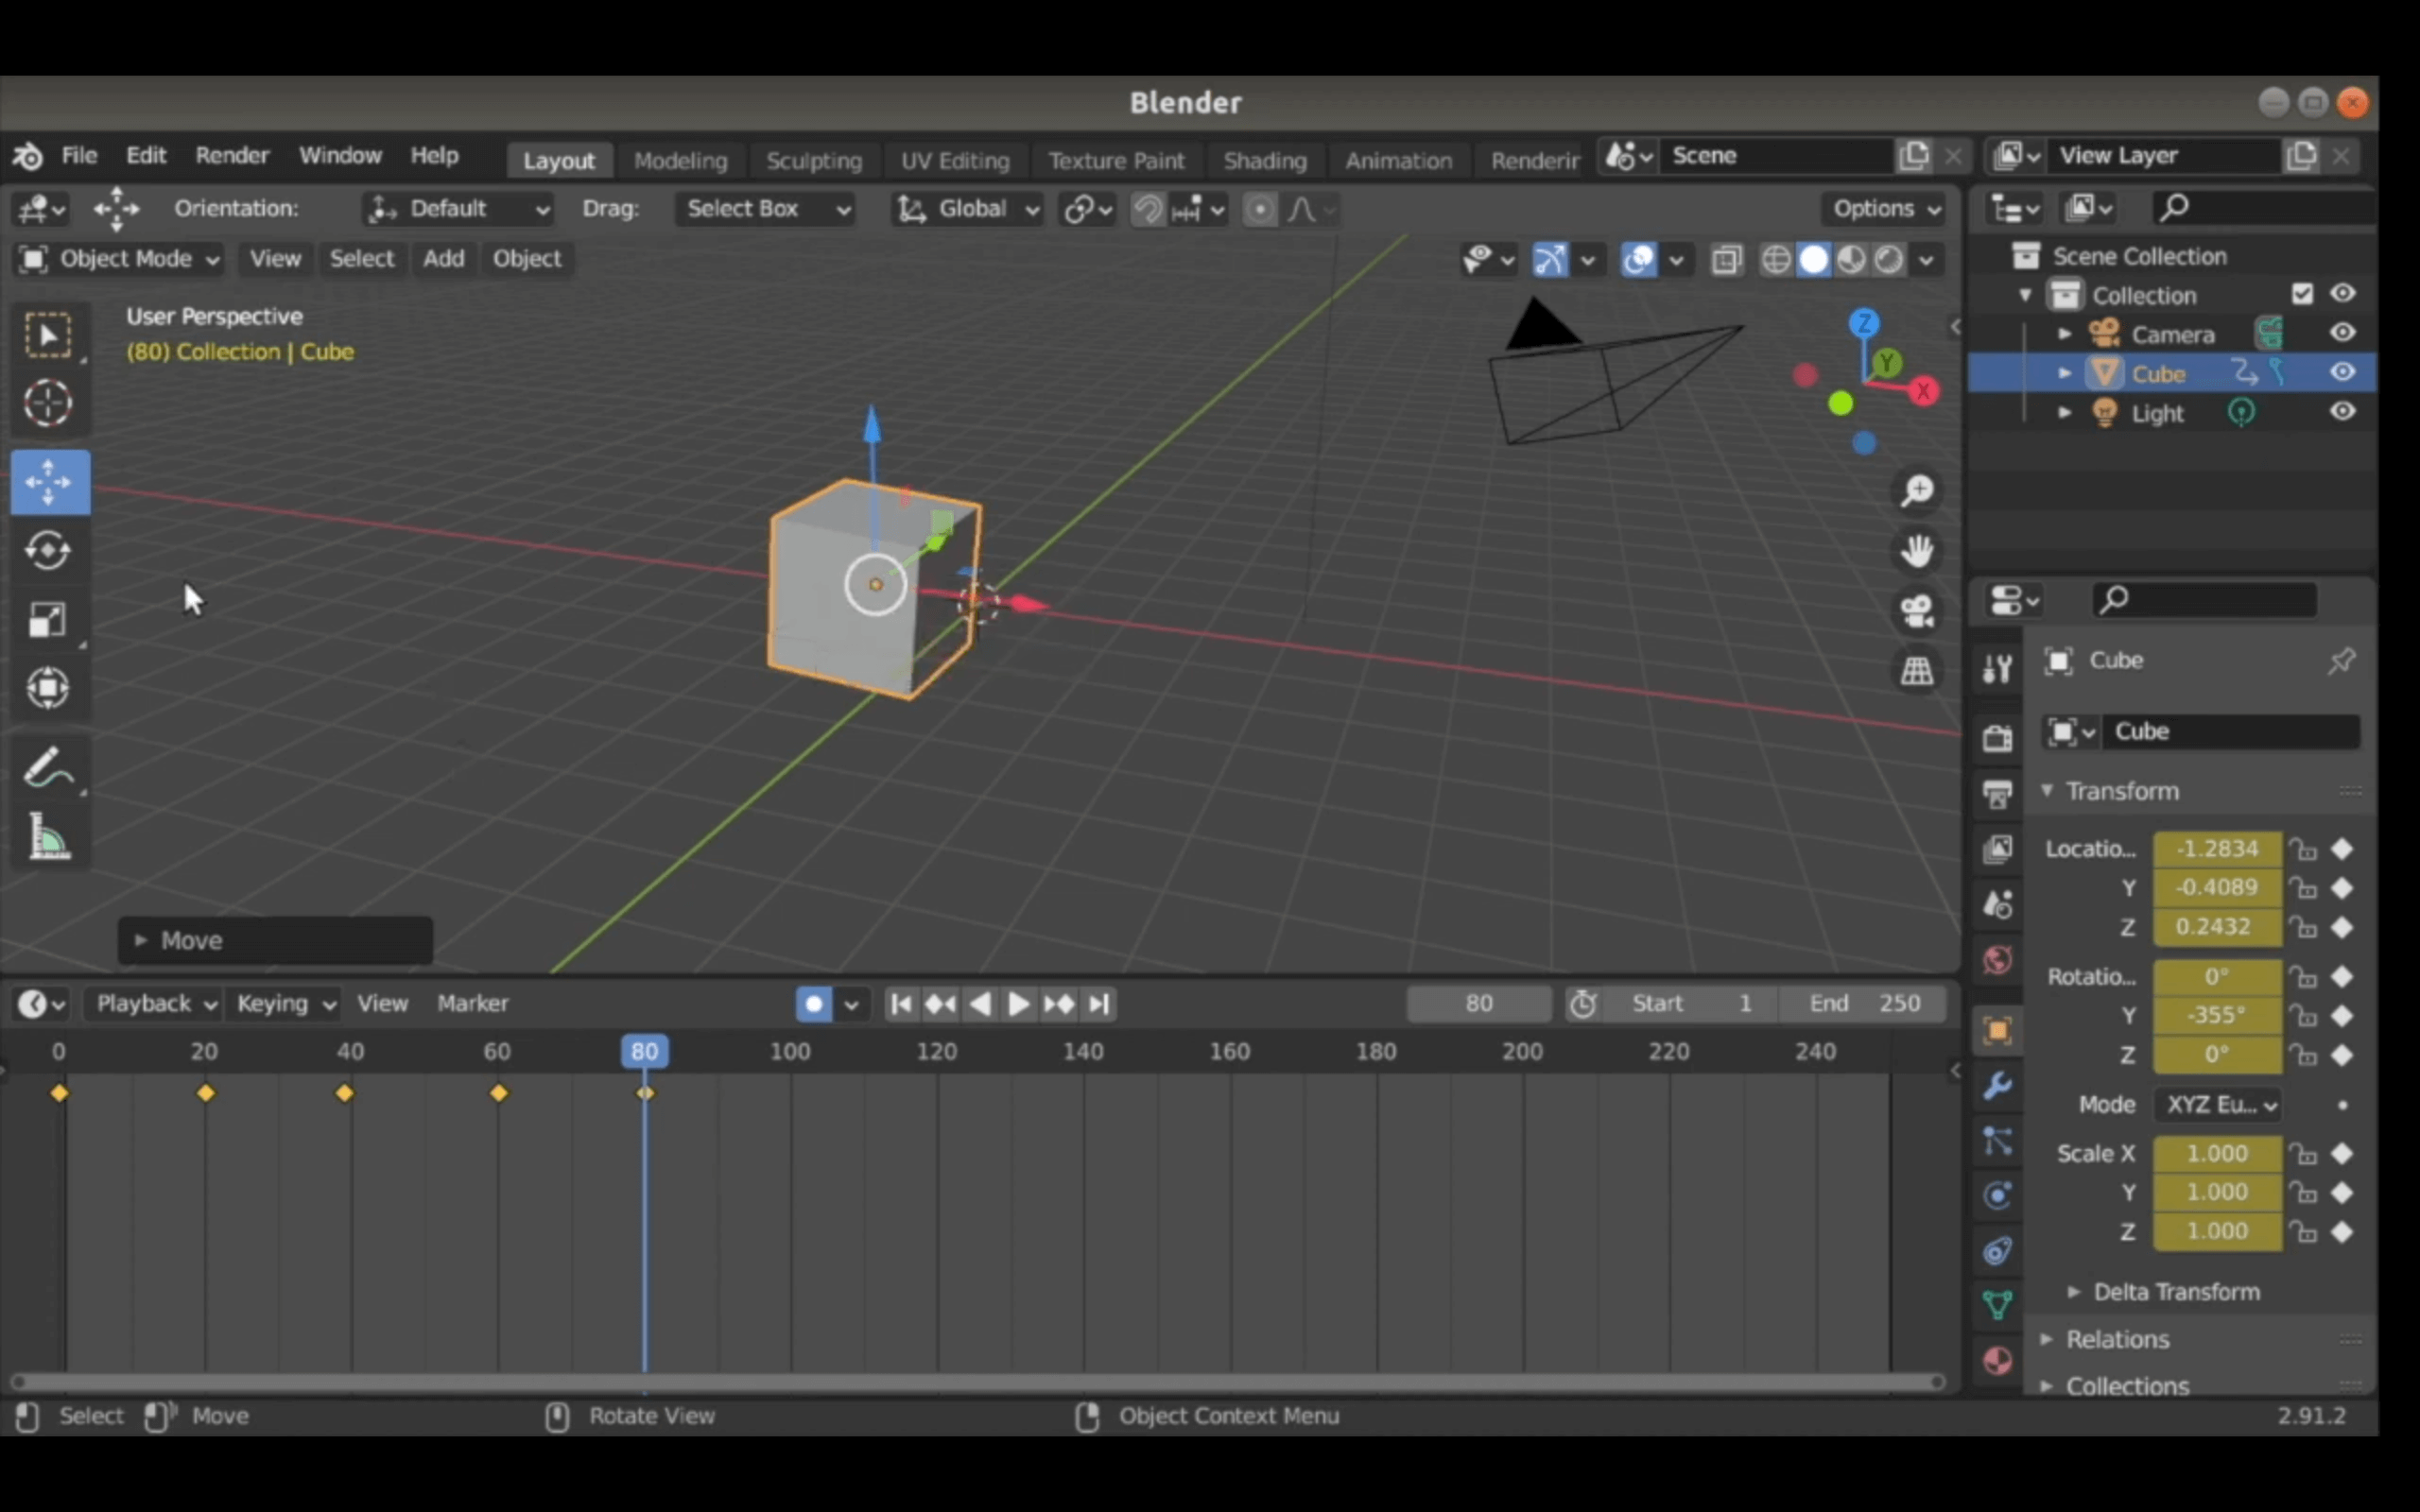
\includegraphics[width=0.7\textwidth, height=0.4\textwidth]{chapters/images/blender.png}
    \caption{Blender}
    \label{fig:my_label}
\end{figure}

\subsection{Plataforma Kibotics}

Kibotics es una plataforma web para docencia en robótica y programación. Esta plataforma se basa en tecnologías web como Django para la parte servidor y utiliza un simulador llamado Websim que se apoya en A-Frame para representar los escenarios de los ejercicios en el navegador del usuario.

Esta plataforma en línea ofrece contenidos educativos para facilitar el aprendizaje en programación a alumnos de primaria, secundaria y bachillerato. Ofrece cursos en lenguajes Scratch y Python. Los ejercicios están disponibles tanto para robots físicos como simulados. Destacan Mbot, Dron Tello y Pibot entre otros.
También ofrece interacción social gracias a un foro.

La simulación de robots reales permite  depurar el software al máximo antes de ejecutarlo en un robot físico y así reducir los costes, ya que no necesitas tener un robot para cada alumno y evitar  posibles daños de los robots y accidentes.

Para usar esta plataforma no es necesario instalar nada, solo tener acceso a Internet. Al ser una aplicación web tenemos la ventaja de que es multiplataforma y podemos usarla en distintos dispositivos.

Kibotics tiene la filosofía \textit{Learn by doing}, aprender haciendo. Las lecciones de teoría junto ejercicios prácticos hacen que los contenidos educativos se vayan adaptando según la complejidad de cada ejercicio. En la Figura 3.9 podemos ver algunos de los ejercicios que ofrecen.

\begin{figure}[H]
\begin{subfigure}{.5\textwidth}
  \centering
  % include first image
  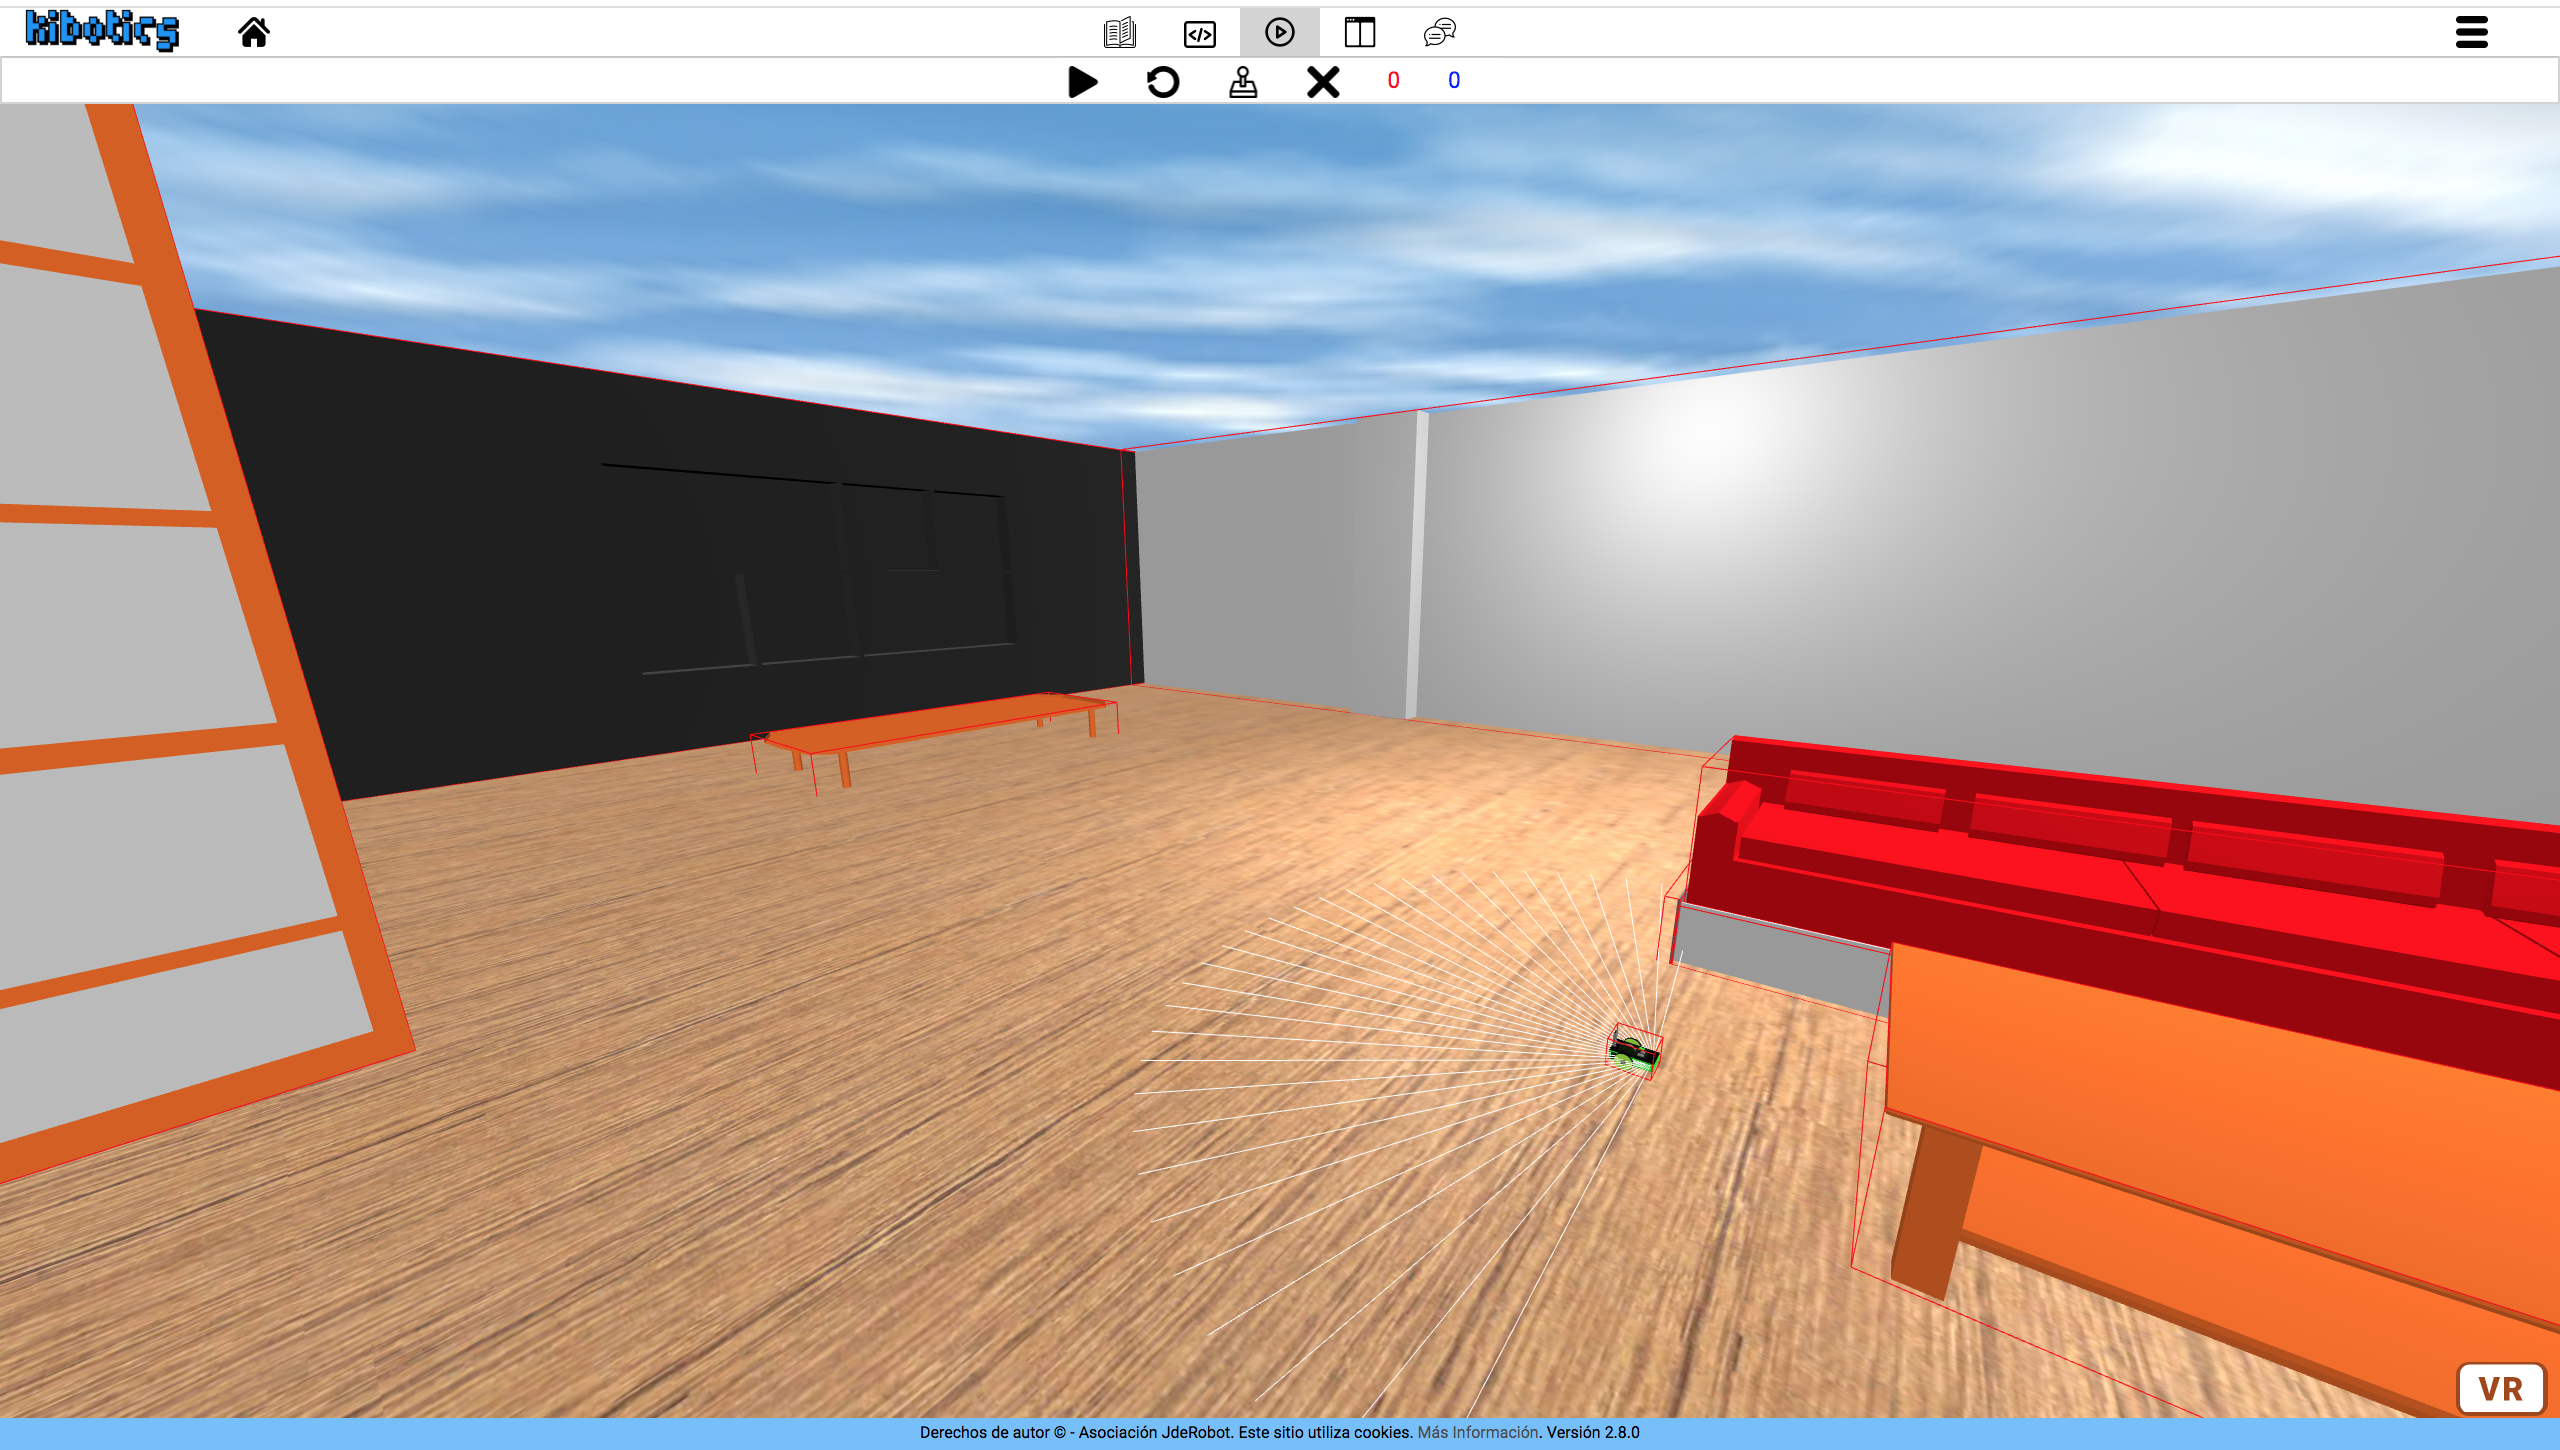
\includegraphics[width=.95\linewidth]{chapters/images/chocagira.png}  
  \caption{Choca-gira US}
  \label{fig:sub-first}
\end{subfigure}
\begin{subfigure}{.5\textwidth}
  \centering
  % include second image
  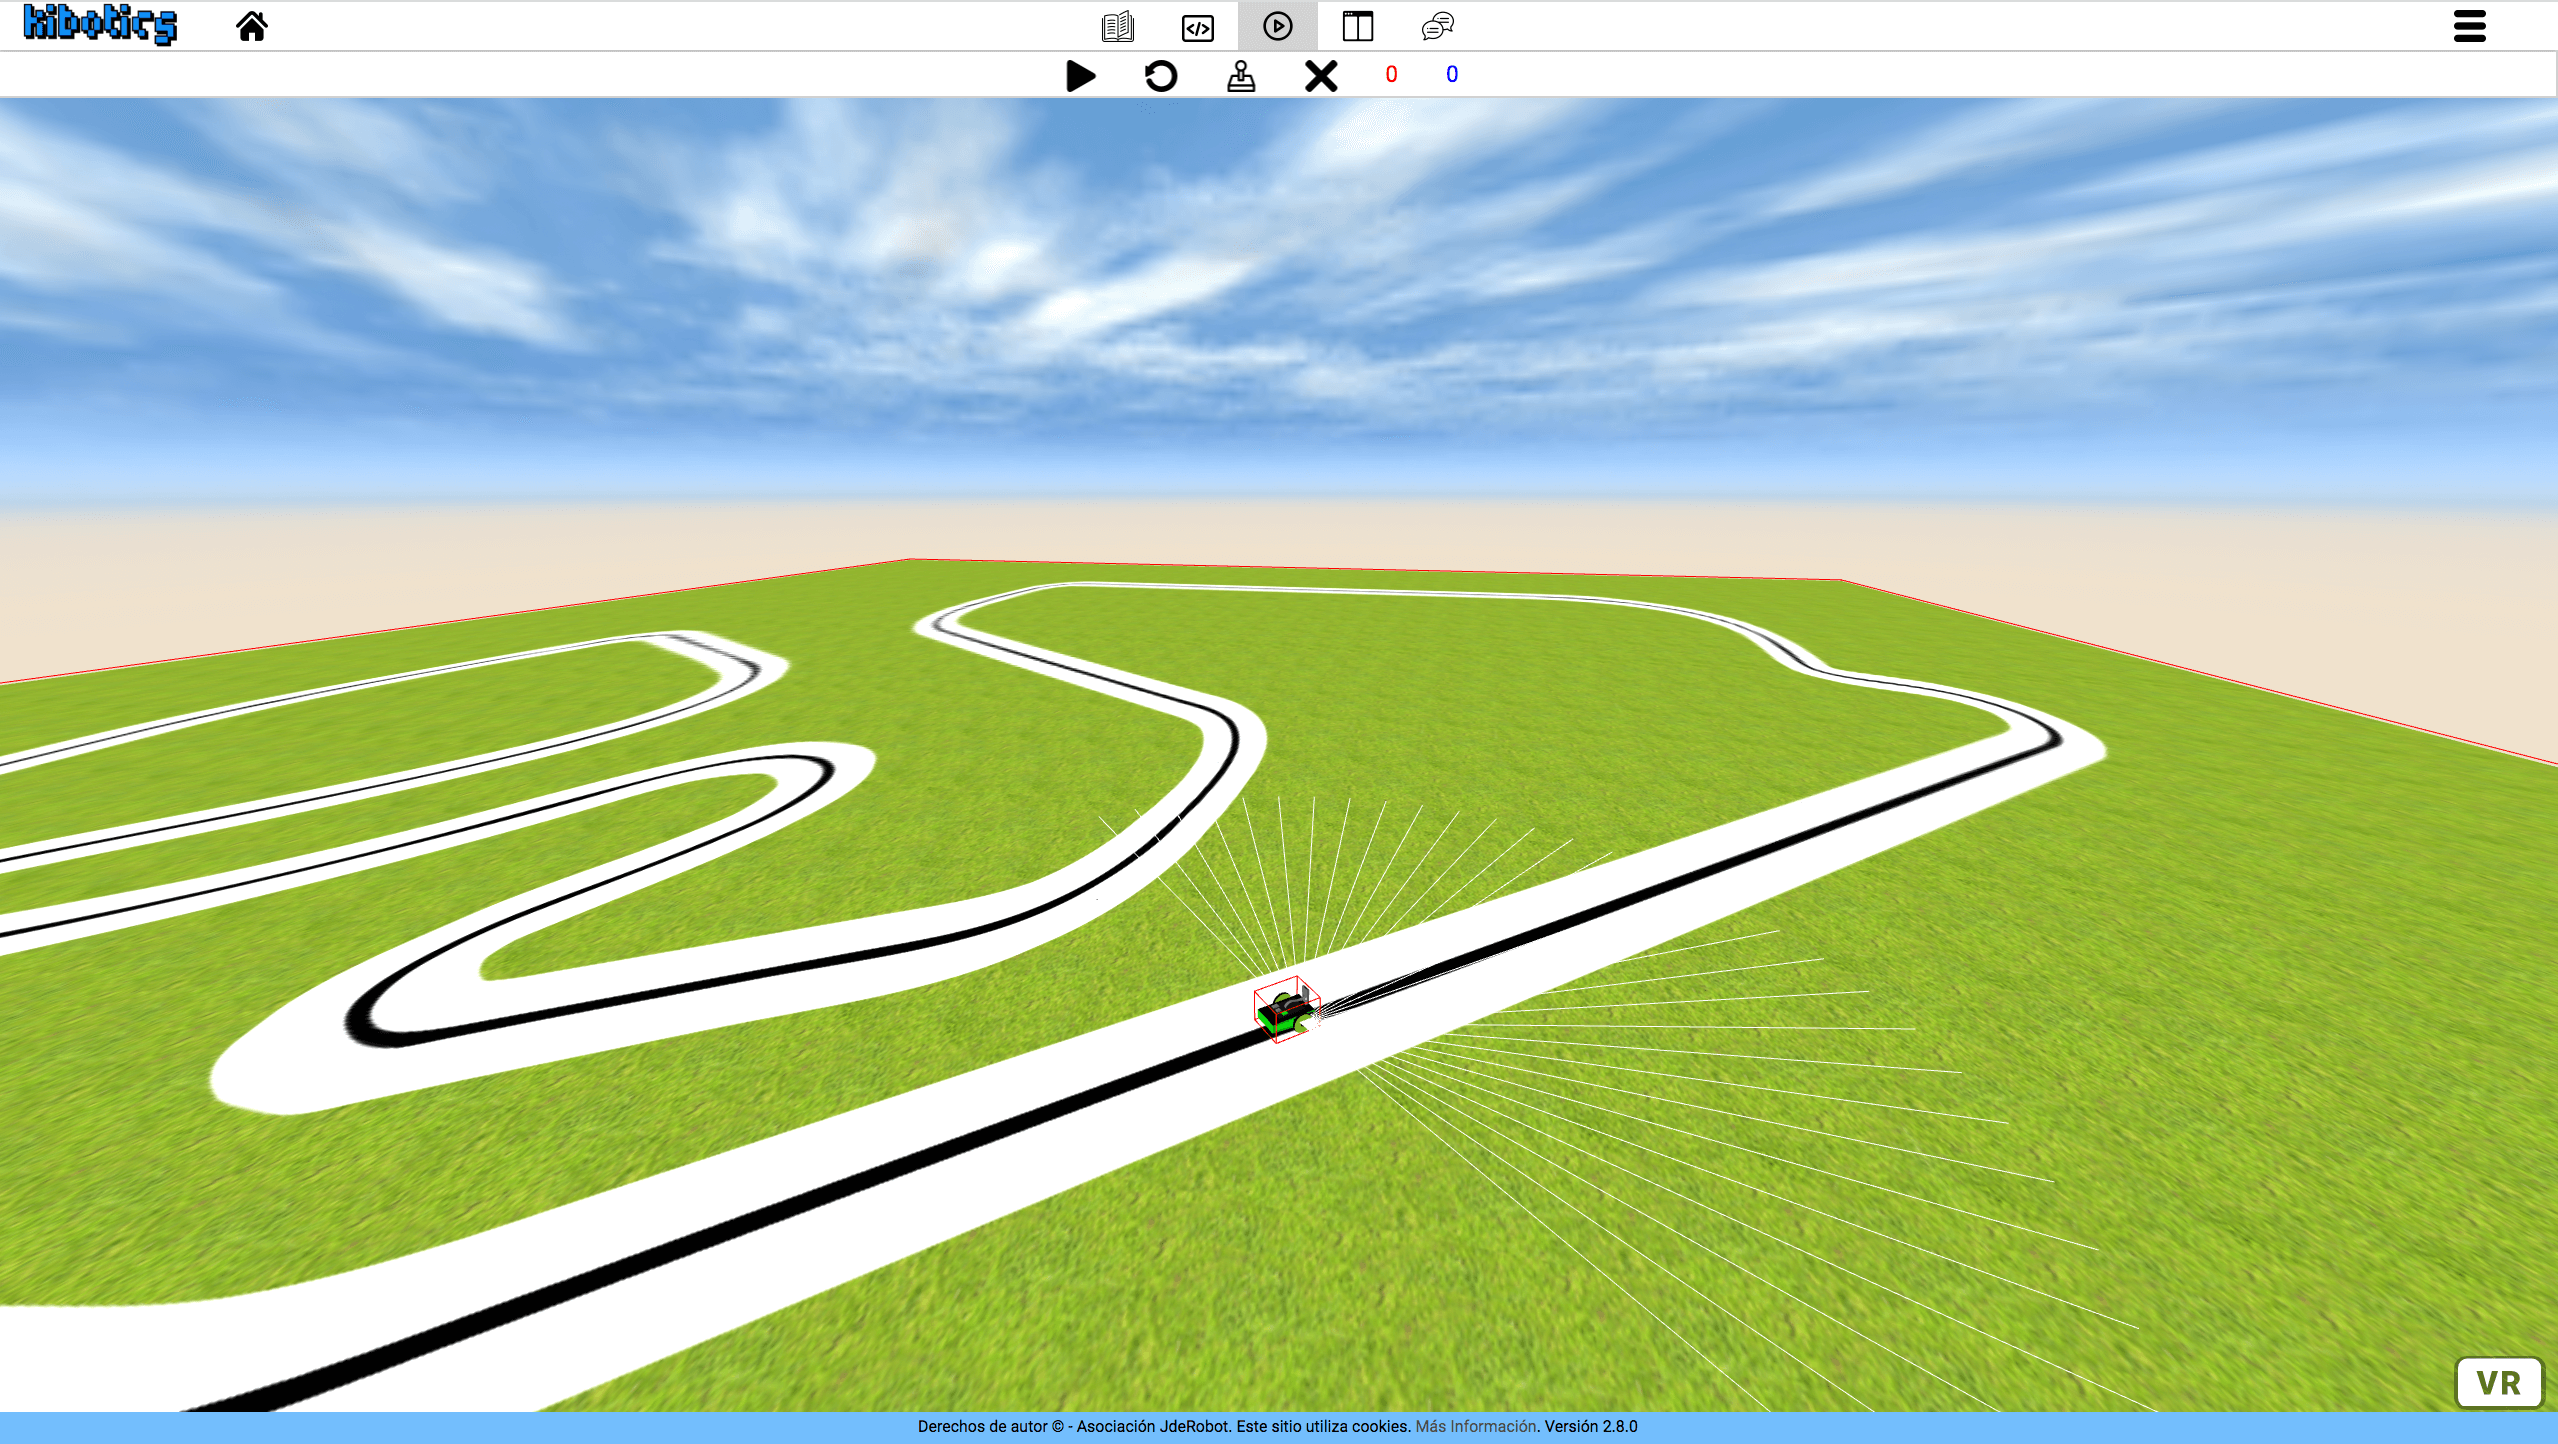
\includegraphics[width=.95\linewidth]{chapters/images/siguelineasir.png}  
  \caption{Sigue líneas IR}
  \label{fig:sub-second}
\end{subfigure}
\begin{subfigure}{.5\textwidth}
  \centering
  % include third image
  \includegraphics[width=.95\linewidth]{chapters/images/atraviesabosque.png}  
  \caption{Atraviesa Bosque}
  \label{fig:sub-third}
\end{subfigure}
\begin{subfigure}{.5\textwidth}
  \centering
  % include fourth image
  \includegraphics[width=.95\linewidth]{chapters/images/colores.png}  
  \caption{Sigue objeto con visión}
  \label{fig:sub-fourth}
\end{subfigure}
\caption{Ejercicios Kibotics}
\label{fig:partes robot}
\end{figure}


Kibotics en los últimos años ha ofrecido cursos para la escuela de pensamiento computacional INTEF, el ayuntamiento de Fuenlabrada, la empresa Logix5, Universidad Rey Juan Carlos, IES Martinez Uribarri (Salamanca) y la Comunidad de Madrid \cite{kiboticspdf}.


\subsection{Navegadores web utilizados}

En este Trabajo Fin de Grado se han usado los navegadores Chrome y Firefox por ser los navegadores más extendidos y que proporcionan gran rendimiento, estabilidad y seguridad. Se han utilizado para la visualización de la página web de Kibotics y la ejecución y pruebas de los distintos ejercicios. 


\chapter{Ejercicio teleoperador acústico y banda sonora}\label{audio}
En los siguientes capítulos se explican los ejercicios desarrollados en este trabajo fin de grado. El primero de ellos es el teleoperador acústico. En este capítulo se nombran las herramientas utilizadas y cómo se ha realizado este ejercicio. También se muestra cómo se ha añadido la posibilidad de incluir efectos de sonido y bandas sonoras a los ejercicios ya existentes. 

\section{Teleoperador Acústico}
\subsection{Enunciado}
En este ejercicio se va a desarrollar un teleoperador acústico. El objetivo es crear un algoritmo de reconocimiento de voz con JavaScript, para poder dirigir un robot de Kibotics con la voz. 

El alumno deberá indicarle  al robot órdenes claras para que él reconozca cada orden  y pueda moverse por el escenario. Hay dos escenarios disponibles, un muro de piedra y una portería de rugby, el robot elegido es un dron que deberá moverse por el mundo sin chocar con ellos.

\subsection{Desarrollo del ejercicio}

Para empezar con este ejercicio se utilizó un fichero de configuración sencillo en el que sólo aparece un dron y un plano con una textura de césped. Este fichero es necesario para que el simulador Websim construya la escena 3D. El fichero de configuración está escrito en JSON y Websim lo analiza para construir los mundos con A-Frame. 
Ésta sería una parte de ese fichero donde se muestra la configuración de la escena \textit{(scene)}, los robots \textit {(robots\_config)}, las texturas \textit{(assets)} y los objetos \textit{(objects)}.

\begin{lstlisting}
{
    "scene-parent-id": "myIFrame",
    "scene": {
        "id": "scene",
        "gravity": 0,
        "sky": "../../assets/textures/sky.png",
        "background": "color: gray;",
        "inspector": "url: https://aframe.io/releases/0.4.0/aframe-inspector.min.js",
        "embedded": true,
        "physics": "debug: true"
    },
    "robots_config": [
        {
            "controller": "user1",
            "id": "a-pibot"
        }
    ],
    "assets": [
        {
            "tag": "img",
            "attr": {
                "id": "ground",
                "alt": "Texture for the scene ground",
                "src": "../../assets/textures/escenarioLiso-min.png"
            }
       ],
    "objects":[
     
        {
            "tag": "a-plane",
            "attr": {
                "static-body": {
                    "mass": 100000
                },
                "position": { "x":0, "y":0, "z":0 },
                "rotation": { "x":-90, "y":0, "z":0 },
                "width": "100",
                "height": "100",
                "src":"#ground"
            }
        },
        {
            "tag": "a-robot",
            "attr": {
                "id": "a-pibot",
                "gltf-model":"../../assets/models/drone_animation.gltf",
                "scale": { "x":0.5, "y":0.5, "z":0.5},
                "position": { "x":0, "y":4, "z":0},
                "rotation": { "x":0, "y":90, "z":0},
                "dynamic-body":{"mass": 1}

            },      
  }
\end{lstlisting}


Una vez creada la escena del ejercicio, se han estudiado 3 herramientas de procesamiento de audio: Web Audio API, TensorFlow JS y Teachable Machine. Todo el desarrollo del teleoperador acústico se ha realizado en JavaScript.

Web Audio API permite escoger fuentes de audio, agregar efectos de sonido, crear visualizaciones, efectos espaciales, filtros y grabaciones, entre otras cosas.
Se estudió la  posibilidad de hacer una red neuronal con esta API. Con esta tecnología se hizo un grabador donde el audio se grababa temporalmente en la memoria del navegador y un analizador en frecuencia en tiempo real \cite{waa2} .  En estos vídeos se puede ver el grabador \footnote{https://www.youtube.com/watch?v=u9aerlWpCdM} y el analizador \footnote{https://www.youtube.com/watch?v=OZk4l7WFTZw} mencionados anteriormente.

Web Audio API es muy útil para visualizado y efectos de sonido pero no nos proporcionaba la suficiente información para poder hacer procesamiento de audio y reconocer palabras, por lo cual se estudiaron otras alternativas para realizar el teleoperador acústico. 

TensorFlow JS es una biblioteca de JavaScript para el aprendizaje automático. Esta herramienta se utiliza para clasificación de imágenes, detección de objetos, segmentación del cuerpo, estimación de pose, detección de rostros y, entre otras, aplicaciones de reconocimiento y clasificación de comandos de voz \cite{tensorflowmodel}.

Para empezar a entender cómo funcionan los modelos, capas y  tensores, en definitiva,  las redes neuronales en esta biblioteca, se realizaron distintos tutoriales de Youtube y de TensorFlow JS tanto de clasificación de imágenes como de reconocimiento de audio. En este video \footnote{https://www.youtube.com/watch?v=x8sUG1CyLdc} se ven las diferentes pruebas que se hicieron. En la Figura 4.1 se puede ver un ejemplo de modelo de detección de objetos.

\begin{figure}[H]
    \centering
    \includegraphics[width=0.8\textwidth, height=0.4\textwidth]{chapters/images/imagerecognition.png}
    \caption{TensorFlow JS ejemplo detección de objetos. }
    \label{fig:my_label}
\end{figure}

Con TensorFlow JS se hicieron dos prototipos. El primero se realizó con un modelo pre-entrenado que reconocía 10 palabras entre ellas go, stop, right, left y seven (que se utilizó para que el robot fuera hacia atrás).
Este modelo al ser pre-entrenado y definido por TensorFlow JS no era muy exacto y el ruido de fondo afectaba demasiado a la hora de detectar cada palabra en nuestro ejercicio. Por ello, el segundo prototipo se hizo con un modelo que se entrenaba con la voz del alumno que usara ese ejercicio.

En este segundo prototipo cada palabra necesitaba grabar sus muestras, al menos unas 100 muestras por palabra, incluidas las muestras de ruido de fondo para que la detección fuera más precisa. Este modelo funcionaba más o menos bien pero no era lo más adecuado para el ejercicio que se había planteado. A pesar de que funcionaba bien se descartó porque era una tarea muy laboriosa grabar todas las muestras cada vez que entrabas en el ejercicio. 
En estos videos \footnote{https://www.youtube.com/watch?v=DcwJzCOE4kI}
\footnote{https://www.youtube.com/watch?v=nPeCAb47jiU}se puede ver  como era el modelo.

Investigando el mundo de reconocimiento de audio y JavaScript se descubrió la herramienta Teachable Machine, la tecnología  que finalmente se ha usado en este proyecto.

Teachable Machine es una herramienta basada en la Web para crear modelos de aprendizaje automático destaca por modelos de clasificación de imágenes, sonidos y posturas. Teachable Machine internamente usa TensorFlowJS . 

La creación de un modelo en Teachable Machine tiene 3 fases: recopilación, preparación y exportación del modelo a tu proyecto.

\begin{itemize}
\item \textit{Recopilación :}

Para hacer el modelo primero hay que recopilar muestras, para ello fue necesaria la participación de 10 personas para que el modelo fuera más completo y pudiera reconocer la palabra independientemente de si la voz del usuarios es más aguda o más grabe.  Se usaron aproximadamente 10 muestras de cada palabra por persona. El modelo cuenta con 105 muestras por cada palabra (10 muestras x 10 personas). Las palabras que queremos reconocer son \textit{go, stop, back, right, left, up, down } y el ruido de fondo. Esto ha supuesto un total de 840 muestras.

Las muestras se grabaron una a una en la página de creación de modelos de Teachable Machine en la Figura 4.2 se puede ver el modelo y las muestras grabadas.


\begin{figure}[H]
 \centering
    \includegraphics[width=0.8\textwidth, height=0.4\textwidth]{chapters/images/teachablemachine.png}
    \caption{Modelo realizado en Teachable Machine}
\end{figure}
 

\item  \textit{Preparación :}

Una vez conseguidas todas las muestras, hay que preparar el modelo. Teachable Machine permite cambiar las épocas. Gracias a unas tablas de precisión y pérdidas por época puedes guiarte para que en función de tus datos puedas ajustar este parámetro. Para este proyecto se utilizaron los valores predeterminados que nos proporcionaban buenos resultados.

\item  \textit{Exportación del modelo a Websim :}

Una vez preparado, la página muestra una vista previa en el que puedes probar y ver el porcentaje de aciertos de cada palabra y con esto decidir si necesitas añadir más muestras o cambiar los parámetros de tu modelo.  En la Figura 4.3 podemos ver la visualización de prueba.

\begin{figure}[H]
 \centering
    \includegraphics[width=0.4\textwidth, height=0.6\textwidth]{chapters/images/teachablemachine2.png}
    \caption{Vista previa del modelo}
\end{figure}
 

Una vez ajustado y con las 105 muestras por palabra, se exportó el modelo. 
Para exportarlo, Teachable Machine lo puede alojar en sus servidores y proporcionarte  un enlace de forma gratuita o puedes descargarlo, se optó por alojarlo en la nube de Teachable Machine para que no ocupara mucho espacio en Kibotics, ya que la forma de importarlo  a JavaScript era similar en ambas opciones.
Una vez subido a la nube, Teachable Machine te proporciona una URL de la dirección de tu modelo y  te proporciona el código necesario para importarlo a tu proyecto desde JavaScript.
\end{itemize}

Con estos 3 pasos ya tenemos creado nuestro modelo en Teachable Machine. Para probar el funcionamiento de este modelo se hizo una prueba de reconocimiento de audio sin fusionarlo con el comportamiento del robot en Websim. En este enlace \footnote{https://martaquintana.github.io/Audio\_Recognition/index.html} se puede probar el funcionamiento de este código basado en HTML5, CSS3, JavaScript y Teachable Machine(TensorFlowJS) (Ver Figura 4.4). Esta página web pide permiso para acceder al micrófono y cuando lo tiene, analiza el audio  y muestra la probabilidad de cada palabra en tiempo real.  

Este es el código de esa página web de prueba del modelo en el que se incluye el código que nos facilita Teachable Machine a la hora de exportar el modelo:

\begin{lstlisting}
<html>
<head>
  <script src="https://cdn.jsdelivr.net/npm/@tensorflow/tfjs@1.3.1/dist/tf.min.js"></script>
  <script src="https://cdn.jsdelivr.net/npm/@tensorflow-models/speech-commands@0.4.0/dist/speech-commands.min.js"></script>
  <style type="text/css">
    button{
      text-decoration: none;
      padding: 10px;
      font-weight: 600;
      font-size: 20px;
      color: #ffffff;
      background-color: #AAA;
      border-radius: 6px;
      border: 2px solid black;
    }
    button:hover{
      color: black;
      background-color: #ffffff;
    }
    button:active {
    box-shadow: 0 2px #666;
    transform: translateY(2px);
  }

  </style>
</head>
<body>

<div>Teachable Machine Audio Model</div>
<button type="button" onclick="init()">Start</button>
<h3 id = "prediction" > The most probable word: </h3>
<div  id="label-container"  style="background-color: #D3D3D3;"></div>

<script type="text/javascript">
    // more documentation available at
    // https://github.com/tensorflow/tfjs-models/tree/master/speech-commands

    // the link to your model provided by Teachable Machine export panel
    const URL = "https://teachablemachine.withgoogle.com/models/P3XdF5r5d/";

    async function createModel() {
        const checkpointURL = URL + "model.json"; // model topology
        const metadataURL = URL + "metadata.json"; // model metadata

        const recognizer = speechCommands.create(
            "BROWSER_FFT", // fourier transform type, not useful to change
            undefined, // speech commands vocabulary feature, not useful for your models
            checkpointURL,
            metadataURL);

        // check that model and metadata are loaded via HTTPS requests.
        await recognizer.ensureModelLoaded();

        return recognizer;
    }

    async function init() {
        const recognizer = await createModel();
        const classLabels = recognizer.wordLabels(); // get class labels
        const labelContainer = document.getElementById("label-container");
        const word = document.getElementById("prediction");
        for (let i = 0; i < classLabels.length; i++) {
            labelContainer.appendChild(document.createElement("div"));
        }

        // listen() takes two arguments:
        // 1. A callback function that is invoked anytime a word is recognized.
        // 2. A configuration object with adjustable fields
        recognizer.listen(result => {
            const scores = result.scores; // probability of prediction for each class
            var word_index = 0;
            // render the probability scores per class
            for (let i = 0; i < classLabels.length; i++) {
                const classPrediction = classLabels[i] + ": " + result.scores[i].toFixed(2);
                labelContainer.childNodes[i].innerHTML = classPrediction;
                //The most probable word
                if (result.scores[i].toFixed(2) >= result.scores[word_index].toFixed(2)) {
                   word_index = i;

                }
            }
            var prediction = classLabels[word_index];
            word.innerHTML = "The most probable word: " + prediction;
            //console.log(prediction);
        }, {
            includeSpectrogram: true, // in case listen should return result.spectrogram
            probabilityThreshold: 0.75,
            invokeCallbackOnNoiseAndUnknown: true,
            overlapFactor: 0.50 // probably want between 0.5 and 0.75. More info in README
        });

        // Stop the recognition in 5 seconds.
        // setTimeout(() => recognizer.stopListening(), 5000);
    }
</script>
</<body>
</html>

\end{lstlisting}


\begin{figure}[H]
    \centering
    \includegraphics[width=0.8\textwidth, height=0.4\textwidth]{chapters/images/audioprueba.png}
    \caption{Página web de prueba de reconocimiento de audio}
    \label{fig:my_label}
\end{figure}

Una vez se comprobó que el modelo funcionaba, se incorporó  el modelo de reconocimiento de audio a Websim, para ello  se creó el siguiente fichero audio.js que se importa en el HTML del ejercicio de la siguiente forma:   

\textless script type=``text/javascript" src=``js/audio.js" \textgreater

Código de audio.js:

\begin{lstlisting}
document.addEventListener('robot-loaded', (evt)=>{
  localRobot = evt.detail;
  console.log(localRobot);
});
// more documentation available at
// https://github.com/tensorflow/tfjs-models/tree/master/speech-commands

// the link to your model provided by Teachable Machine export panel
const URL = "https://teachablemachine.withgoogle.com/models/P3XdF5r5d/";
var connection = false;
var noise_times = 0;

async function createModel() {
    const checkpointURL = URL + "model.json"; // model topology
    const metadataURL = URL + "metadata.json"; // model metadata

    const recognizer = speechCommands.create(
        "BROWSER_FFT", // fourier transform type, not useful to change
        undefined, // speech commands vocabulary feature, not useful for your models
        checkpointURL,
        metadataURL);

    // check that model and metadata are loaded via HTTPS requests.
    await recognizer.ensureModelLoaded();

    return recognizer;
}

async function analizar(recognizer,classLabels,word) {
//  for (let i = 0; i < classLabels.length; i++) {
  //    labelContainer.appendChild(document.createElement("div"));
  //}

  // listen() takes two arguments:
  // 1. A callback function that is invoked anytime a word is recognized.
  // 2. A configuration object with adjustable fields
  recognizer.listen(result => {
      console.log(noise_times)
      const scores = result.scores; // probability of prediction for each class
      var word_index = 0;

      // render the probability scores per class
      for (let i = 0; i < classLabels.length; i++) {
          const classPrediction = classLabels[i] + ": " + result.scores[i].toFixed(2);
          //labelContainer.childNodes[i].innerHTML = classPrediction;
          //The most probable word
          if (result.scores[i].toFixed(2) >= result.scores[word_index].toFixed(2)) {
             word_index = i;
          }
      }
      var prediction = classLabels[word_index];
      word.innerHTML = "The most probable word: " + prediction;
      if (String(prediction) == "_background_noise_"){
        noise_times = noise_times + 1;
      }else{
        noise_times = 0;
      }
      if (connection){
        if (String(prediction) == "Go") {
          localRobot.setV(0.9);
          //que se mueva el robot
        }else if (String(prediction) == "Stop") {
           localRobot.setV(0);
           localRobot.setW(0);
           localRobot.setL(0);
          //que se pare
        }else if (String(prediction) == "Back"){
           localRobot.setV(-0.9);
        }else if (String(prediction) == "Right"){
            localRobot.setW(-0.005);

        }else if (String(prediction) == "Left"){
            localRobot.setW(0.005);

        }else if (String(prediction) == "Up"){
            localRobot.setL(0.25);

        }else if (String(prediction) == "Down"){
            noise_times = 0;
            console.log(localRobot.velocity);
            if (localRobot.velocity.y = 0.25) {
              localRobot.setL(-0.25);
            }
        }
        //For stop going down or going up, turn left or turn right say the word : STOP

      }
      //console.log(prediction);
  }, {
      includeSpectrogram: true, // in case listen should return result.spectrogram
      probabilityThreshold: 0.75,
      invokeCallbackOnNoiseAndUnknown: true,
      overlapFactor: 0.50 // probably want between 0.5 and 0.75. More info in README
  });

  // Stop the recognition in 10 seconds.
  setTimeout(() => {recognizer.stopListening(); }, 10000);

}

async function listen() {
        document.getElementById("listen_again").style.visibility = 'hidden';
        //--------TEACHABLE MACHINE--------------
        const recognizer = await createModel();
        const classLabels = recognizer.wordLabels(); // get class labels
        //const labelContainer = document.getElementById("label-container");
        const word = document.getElementById("prediction");
      //  for (let i = 0; i < classLabels.length; i++) {
        //    labasync function listen() {elContainer.appendChild(document.createElement("div"));
        //}

       var id = setInterval(() => {if(noise_times <= 10){analizar(recognizer,classLabels,word)}else{
          setTimeout(() => {console.log("Se ha parado de analizar")
            word.innerHTML = "The most probable word: " ;
            clearInterval(id);
            document.getElementById("listen_again").style.visibility = 'visible';
            //Robot Control opcional
            //localRobot.setV(0);
            //localRobot.setW(0);
            //localRobot.setL(0);
          }, 10000);
        }}, 10150);

}

async function Back\_To\_Listen(){
   document.getElementById("prediction").innerHTML= 'The most probable word: <br> <img src="https://wbl.telcel\-id.com:8443/images/Load\_Icon.gif" alt="Loading the model">'
   noise\_times = 0;
   listen();
}

async function Connect\_To\_Robot() {
    if (connection){connection= false;
      document.getElementById("connection").style.backgroundColor= "red";
      console.log( "Desconectado");
    }else{
        connection = true;
        listen();
        console.log( "CONECTADO AL ROBOT");
        document.getElementById("connection").style.backgroundColor= "green";
    }
}
\end{lstlisting}

Con el fichero de configuración, el HTML y este código JavaScript el ejercicio se visualiza como se muestra en la Figura 4.5.

\begin{figure}[H]
    \centering
    \includegraphics[width=0.8\textwidth, height=0.4\textwidth]{chapters/images/audio.png}
    \caption{Ejercicio teleoperador acústico}
    \label{fig:my_label}
\end{figure}

A continuación se explica como funciona este programa.

Cuando se pulsa al boton Conect\_To\_Robot se llama a la función del mismo nombre que internamente ejecuta  la funcion listen() que es la que inicializa el reconocimiento y analiza el audio cada 10 segundos.
Este botón se pone en verde cuando esta analizando y en rojo cuando está desconectado, esto quiere decir que el robot no reconoce ninguna palabra mientras el botón esté de ese color.

La función listen() inicializa el modelo y crea las etiquetas que necesita, se ha creado un setTimeout para esperar 10 segundos hasta que cargue el modelo. Cuando este carga, se establece un setInterval para que cada 10 segundos se ejecute la función analizar que devuelve la palabra estimada.

La función analizar es la que invoca al analizador o \textit{recognizer}, en él se predice la palabra que cree que es más probable que haya dicho el usuario.  \textit{Prediction} es esa palabra que tiene  la probabilidad más alta.

Una vez tenemos la \textit{prediction} se compara esta palabra con las 8 palabras que hemos entrenado el modelo \textit{go, stop, back, right, left, up, down y \_background\_noise\_}

Gracias al evento 'robot-loaded' cuando el robot está cargado en el escenario,  obtenemos el objeto localRobot, que en nuestro ejercicio es el dron. En Kibotics poseen una API\footnote{Application Programming Interfaces} llamada HAL API \footnote{Hardware Abstraction Layer} con funciones para controlar el movimiento del robot.  Cuando se predice una de las 8 palabras en los condicionales \textit{if(){} else if() {}}se llama a una de estas funciones de velocidad : localRobot.setV(), para asignar la velocidad lineal, se utiliza para ir hacia delante ``go'', ir hacia atrás ``back '' o parar ``stop'',  localRobot.setW() para la velocidad angular, se usa para girar a la derecha``right'' o a la izquierda``left'' y  localRobot.setL() para asignar la velocidad que va a subir ``up'' o bajar ``down'' el dron. Si se predice que es ruido de fondo no afecta en el comportamiento del dron.

La implementación del ejercicio con Teachable Machine  nos ha aportado sencillez y más precisión que los modelos mencionados anteriormente.
Una vez realizado el ejercicio se optimizó para que el navegador del usuario no estuviera todo el tiempo analizando el  audio si no tenemos nada que decirle al dron y aprovechar los recursos del ordenador del usuario.

La optimización se realizó añadiendo el contador \textit{(noise\_times)} que aparece en el código anterior, este cuenta las veces que se predice ruido de fondo. Se estableció un máximo de 10 las veces seguidas que la predicción es \textit{\_background\_noise\_}. Como se analiza el audio cada 10 segundos esto quiere decir que si han pasado 100 segundos y siempre ha detectado ruido de fondo, la función analizar para de ejecutarse y no se predice ninguna palabra. Cuando ocurre esto se muestra en el navegador un nuevo botón \textit{(Continue analizing)} que  si lo pulsas desaparece y se reinicia el procesamiento de audio. Ver Figura 4.6.

\begin{figure}[H]
  \begin{subfigure}[b]{0.5\textwidth}
  \centering
    \includegraphics[width=0.95\textwidth, height=0.7\textwidth]{chapters/images/optimizacionaudio.png}
    \caption{Botón Continue analizing }
    \label{fig:f1}
  \end{subfigure}
  \hfill
  \begin{subfigure}[b]{0.5\textwidth}
  \centering
    \includegraphics[width=0.95\textwidth, height=0.7\textwidth]{chapters/images/optimizacionaudio2.png}
	\caption{Se reinicia el procesamiento de audio.}    
    \label{fig:f2}
 
  \end{subfigure}
  \caption{Optimización del modelo }
\end{figure}


Para este ejercicio se crearon dos escenarios uno con portería de rugby y otro con una pared que se añadieron al  fichero de configuración del drone que hemos visto al principio del capítulo. La portería se creó con Blender y la pared con A-Frame en el fichero de configuración de Websim. Ver Figura 4.7 y 4.8.

 \begin{figure}[H]
  \begin{subfigure}[b]{0.5\textwidth}
  \centering
    \includegraphics[width=0.95\textwidth, height=0.7\textwidth]{chapters/images/porteriablender.png}
    \caption{}
    \label{fig:f1}
  \end{subfigure}
  \hfill
  \begin{subfigure}[b]{0.5\textwidth}
  \centering
    \includegraphics[width=0.95\textwidth, height=0.7\textwidth]{chapters/images/porteriawebsim.png}
	\caption{}    
    \label{fig:f2}
 
  \end{subfigure}
  \caption{Modelos portería en Blender y  en Websim }
\end{figure}


\begin{figure}[H]
\centering
    \includegraphics[width=0.7\textwidth, height=0.5\textwidth]{chapters/images/pared.png}
    \caption{Pared de piedra en Websim}
    \label{fig:f1}
  \end{figure}



\subsection{Solución de referencia}

Este ejercicio es un juego, el objetivo es dirigir al dron con tu voz para cruzar por la portería de rugby o pasar de un lado al otro de la pared sin chocarte con ellas. Se ha realizado un video promocional \footnote{https://youtu.be/sr54MxMw954} y este otro vídeo \footnote{https://www.youtube.com/watch?v=85oTxgQQrck} donde se muestran unas posibles soluciones para guiar al dron en los distintos escenarios.

 \begin{figure}[H]
  \begin{subfigure}[b]{0.5\textwidth}
  \centering
    \includegraphics[width=1\textwidth, height=0.7\textwidth]{chapters/images/solucionaudio.png}
    \caption{}
    \label{fig:f1}
  \end{subfigure}
  \hfill
  \begin{subfigure}[b]{0.5\textwidth}
  \centering
    \includegraphics[width=1\textwidth, height=0.7\textwidth]{chapters/images/solucionaudio2.png}
	\caption{}    
    \label{fig:f2}
 
  \end{subfigure}
  \caption{Ejemplo solución teleoperador acústico}
\end{figure}


\section{Banda Sonora}

Para añadir banda sonora a los ejercicios existentes en Kibotics, se estudió como insertar audio desde HTML5 e implementarlo con JavaScript en Websim.

El elemento HTML \textless audio\textgreater  se usa para reproducir un fichero de audio en una página web.
Los atributos que destacan de este elemento son \textit{controls, source, loop y autoplay }.
El atributo \textit{controls} proporciona controles como reproducir, parar y subir o bajar el volumen.
 \textit{Source} permite especificar la fuente de audio, en este caso un fichero en formato mp3, ogg o wav. \textit{Loop} permite volver a reproducir el audio cuando este se acaba, el audio estará en bucle y \textit{autoplay} se utiliza para que una vez se cargue el fichero de audio, este empiece a reproducirse.

Para hacer esta mejora a Kibotics, en la carpeta assets de Websim se añadió una nueva carpeta llamada ``soundtracks'' con temas musicales para poner en los ejercicios. Las canciones usadas son de Patrick De Artega Royalty Free Music  \footnote{ https://patrickdearteaga.com Credits to Patrick De Artega Royalty Free Music 2020}
y los temas que se han añadido son:
Chiptronical, Common Fight, Goliath's Foe, Resilience, Spring Village, TheTrueStory of Beelzebub y Vals de su jardín


La banda sonora de cada ejercicio se define en su fichero de configuración. En ese fichero se ha creado un objeto con una  la etiqueta ``soundtrack'', el identificador ``audio'' y la dirección del fichero fuente del audio (\textit{src}) que se quiere asignar como banda sonora, como se muestra en el siguiente código:

\begin{lstlisting}
 	{"tag":"soundtrack",
        "attr": {
            "id":"audio",
            "src": "../assets/soundtracks/Spring\_Village.ogg"
          }
        },
   \end{lstlisting}

Websim tiene un analizador de ficheros json llamado config\_parser.js, con este fichero JavaScript se analiza el fichero de configuración (incluyendo el objeto que hemos mencionado anteriormente) y traducirlo a A-Frame.

Cuando Websim lee el fichero de configuración (formato JSON) se llama a parseSoundtrack() que recibe los objetos de la escena para analizar si hay banda sonora o no en el ejercicio.

\begin{lstlisting}
 	await parseSoundtrack(sceneObjects);
\end{lstlisting}

En el siguiente código se muestra como se analizan todos los objetos de la escena y si alguno tiene la etiqueta ``soundtrack'', la variable soundtrack  que por defecto siempre es \textit{false}, pasa a ser \textit{true} y se asigna a la variable audio el atributo  ``src'' del objeto, en este caso ``../assets/soundtracks/Spring\_Village.ogg".  
Si soundtrack es \textit{true}, se crea un objeto Audio() de HTML5 desde JavaScript; y se le asigna el \textit{src} del audio configurado y se empieza a reproducir. Como \textit{reproducir.loop} es \textit{true}, el audio estará en bucle todo el tiempo.

\begin{lstlisting}
export function parseSoundtrack(sceneObjects){
  var soundtrack = false;
  for (var i = 0; i <sceneObjects.length;i++){
   if (sceneObjects[i]['tag']== 'soundtrack'){
     soundtrack = true;
     var audio=sceneObjects[i]['attr']['src'];
    }
  }
  if (soundtrack) {
    var reproducir = new Audio();
        reproducir.src= audio
        reproducir.loop= true;
        reproducir.play();
  }
  return;
}
\end{lstlisting}

En este video \footnote{https://www.youtube.com/watch?v=c\_\_BayBCSX4} se puede escuchar la banda sonora que se ha asignado en un ejercicio de ejemplo.

\subsection{Efecto de sonido por colisión }

Los efectos de sonido son muy importantes en los juegos, es por ello que se pensó mejorar la experiencia del usuario añadiendo el efecto de sonido de colisión. 

Se implementó con el evento \textit{`collide'} de A-Frame. Cuando se detecta una colisión este evento llama a una función que reproduce un audio y pone a 0 todas las velocidades V, W y L del robot.  En este caso la reproducción del audio se hace una vez por choque como pasaría en la realidad.

\begin{lstlisting}
  document.addEventListener('collide', function (e) {
      console.log('Robot has collided!');
      var reproducir = new Audio();
      reproducir.src= 'http://sonidosmp3gratis.com/sounds/000215403\_prev.mp3';   //collision sound
      reproducir.play();
      localRobot.setV(0);
      localRobot.setW(0);
      localRobot.setL(0);
	});
	
\end{lstlisting}

Esta función sirve para todos los ejercicios de la plataforma con o sin  bandas sonoras y para el teleoperador acústico. En el video de las soluciones  \footnote{https://www.youtube.com/watch?v=85oTxgQQrck}  en el escenario de la pared de piedra se puede escuchar el efecto de sonido por colisión cuando el dron choca con la pared.
\chapter{Ejercicio aspiradora robótica atrapa confeti}\label{chap:aspiradora}
En los siguientes capítulos se explica el proceso de desarrollo de los tres ejercicios realizados en este trabajo fin de grado. Este capítulo está dedicado al primero de ellos, este ejercicio consiste en una aspiradora robótica que atrapa piezas de confeti que están dispersas por el suelo de una casa. En primer lugar se expone el enunciado y los objetivos. En segundo lugar cómo se ha implementado y creado los modelos de robot aspiradora y escenario, para la plataforma Kibotics. Finalmente, se muestran las soluciones de referencia creadas en Python y Scratch que satisfacen el objetivo del ejercicio.

Para hacer el ejercicio descrito a continuación, se utilizaron las herramientas Blender, el simulador Websim de Kibotics que contiene la tecnología A-Frame y los lenguajes JavaScript, HTML5 y JSON.

\section{Enunciado}
La finalidad de este ejercicio era programar una aspiradora robótica que se encuentre en una habitación y que ésta fuera capaz de recoger piezas de confeti cuando pase por encima. El evaluador automático que se ha realizado nos servirá para contar el confeti recogido por los usuarios en un tiempo determinado.

El alumno deberá programar en Scratch o en Python un algoritmo de planificación de ruta para que consiga atrapar el mayor número de trozos de confeti en 5 minutos. El objetivo del usuario es que utilice los sensores y actuadores del robot para que cuando detecte un objeto próximo, por ejemplo una pared o una mesa, se mueva en ángulos aleatorios. 

Para la visualización de este ejercicio y que los usuarios de Kibotics puedan acceder a él, se ha creado una página web. Gracias a esta página web, los usuarios tienen acceso a la teoría del ejercicio y  disponen de un editor y el simulador Websim necesarios para hacer el ejercicio. 

La teoría del ejercicio se creó en HTML5 y se modificaron las plantillas que utiliza el servidor Django de Kibotics.
En las siguientes figuras podemos ver la página de teoría donde se explica el objetivo del ejercicio y los requisitos (Figura 4.1). Para explicar al alumno los diferentes algoritmos de cobertura que pueden utilizar los aspiradores robóticos, se ha añadido un poco de teoría sobre esos algoritmos (Figura  4.2), unas pequeñas pistas y un ``¿Sabías que... ? '' (Figura 4.3) hablando de las primeras aspiradoras y cómo funcionaban. 
\\

\begin{figure}[H]
    \centering
    \includegraphics[width=1\textwidth, height=0.5\textwidth]{chapters/images/teoria1.png}
    \caption{Página de teoría enunciado y requisitos}
    \label{fig:my_label}
\end{figure}
\begin{figure}[H]
    \centering
    \includegraphics[width=1\textwidth, height=0.5\textwidth]{chapters/images/teoria2.png}
    \caption{Teoría}
    \label{fig:my_label}
\end{figure}
\begin{figure}[H]
    \centering
    \includegraphics[width=1\textwidth, height=0.5\textwidth]{chapters/images/teoria3.png}
    \caption{Pistas y ¿sabías que.. ?}
    \label{fig:my_label}
\end{figure}

\section{Modelos del mundo}
Para este ejercicio se crearon nuevos muebles con Blender (ver Figuras 4.4 y 4.5) para que el escenario pareciera una habitación realista (ver Figura 4.6).
\begin{figure}[H]
  \begin{subfigure}[b]{0.5\textwidth}
  \centering
    \includegraphics[width=0.95\textwidth, height=0.6\textwidth]{chapters/images/silla.png}
    \caption{Modelo silla}
    \label{fig:f1}
  \end{subfigure}
  \hfill
  \begin{subfigure}[b]{0.5\textwidth}
  \centering
    \includegraphics[width=0.95\textwidth, height=0.6\textwidth]{chapters/images/mesa.png}
	\caption{Modelo mesa}    
    \label{fig:f2}
 
  \end{subfigure}
  \caption{Modelos en Blender}
\end{figure}

\begin{figure}[H]
  \centering
 \includegraphics[width=0.7\textwidth]{chapters/images/sofa.png}
  \caption{Modelo sofá en Blender}
\end{figure}

\begin{figure}[H]
\centering
\includegraphics[width=0.8\textwidth, height=0.4\textwidth]{chapters/images/habitacioncon.png}
\caption{Habitación amueblada}
\end{figure}

Estos objetos se añadieron en el fichero de configuración JSON del ejercicio definiendo su identificador, modelo 3D gltf, la posición y la escala. El código que se muestra a continuación pertenece a la creación de la mesa pero la estructura  de todos los elementos añadidos es la misma: 
\begin{lstlisting}
{    "tag": "a-entity",
          "attr": {
              "id": "model-table",
              "gltf-model":"/static/websim/assets/models/mesa.gltf",
              "position":{"x":40, "y":0,"z":0},
              "scale": {"x":3,"y":3,"z":3}
          }
      },
\end{lstlisting}

También se añadieron a ese fichero de configuración, de forma muy similar, las paredes, una puerta y un cuadro. Se ajustó la posición, dimensiones y texturas correspondientes.

Para que el ejercicio tuviera mayor dificultad se introdujeron 2 pelotas con movimiento. Para conseguir este movimiento se consideraron dos posibilidades: animación desde Blender o animación desde A-Frame. 
En el vídeo \footnote{https://www.youtube.com/watch?v=1JPb3Mw8638}  se puede ver cómo hacer una animación no lineal sencilla en Blender. Para poder usar animaciones de Blender en Websim, es necesario que sean animaciones no lineales. Estudiando ambas opciones, se optó por la animación en A-Frame desde el fichero de configuración, que era el método ideal para Websim. De esta forma dejamos toda la creación de las pelotas, asignación de texturas, posición y  animación definido en la configuración.

Para animar un objeto desde A-Frame añadimos el atributo \textit{``animation"} y completamos los valores necesarios como desde dónde a dónde quieres que se mueva  el objeto o el tiempo que quieres que tarde en hacer esa animación. Por ejemplo, en el siguiente código se puede ver cómo se define la animación en diagonal de la pelota de baloncesto. Las dos pelotas tienen los mismos atributos pero con valores diferentes.
\begin{lstlisting}
  {    "tag": "a-sphere",
            "attr": {
                "id":"basketball",
                "position": { "x":-40, "y":1.5, "z":-40 },
                "rotation": { "x":0, "y":0, "z":0 },
                "radius": 1.5,
                "src":"#basketball",
                "static-body": {
                    "mass": 2
                },              
	           "class":"collidable",
                "animation": "property: position; from: -40 1.5 -40 ;to: 40 1.5 40; dir: alternate; dur: 10000; loop: true"
            }
        },
\end{lstlisting}

En el escenario de este ejercicio se crearon un conjunto de 100 trozos de papel, confeti, repartidos por el suelo. Estos modelos se hicieron con la etiqueta \textit{a-cylinder} de A-Frame.  

El confeti no se crea desde el fichero de configuración, dado que se tendrían que crear uno a uno todos los confetis y extendería demasiado el fichero. Lo que se ha hecho es que, una vez esta cargado el mundo en el navegador del usuario, usando JavaScript, creamos dinámicamente todos los confetis.

Primero se generó un programa para fijar aleatoriamente las posiciones de los confetis en el mundo, así los confetis quedan esparcidos por la habitación. Estas posiciones x, y, z de los confetis se guardaron en otro fichero JSON llamado \textit{data.json}, de esta forma, todos los alumnos cuentan con el mismo escenario. El escenario está formado por 100 confetis de colores y el color de cada uno se elige aleatoriamente cuando se crea desde JavaScript .

Parte del fichero data.json: 
\begin{lstlisting}
  data = '[{"x":-39,"y":0,"z":-14},
                {"x":7,"y":0,"z":-11},
                {"x":-6,"y":0,"z":-9},
                {"x":-33,"y":0,"z":28},
                {"x":-11,"y":0,"z":41},
                {"x":-11,"y":0,"z":-13},
                {"x":19,"y":0,"z":23},
                {"x":19,"y":0,"z":-30},
                {"x":-4,"y":0,"z":-27},
                {"x":25,"y":0,"z":20},
                ....]'
 \end{lstlisting}


Para leer el fichero \textit{data.json} se utiliza éste código en la plantilla HTML del ejercicio.
\begin{lstlisting}
 <script type="text/javascript" src="{\% static '/data.json' \%}"></script > 
 \end{lstlisting}


En el siguiente código podemos ver cómo se crea el confeti con la función \textit{document .createElement(`a\- cylinder')}. Una vez creado se le asignan los atributos con la función  \textit{setAttribute}.  El identificador es confeti más un número  n, n es un número de 0-99 que se le asigna para crear 100 confetis diferentes (ejemplo de id del confeti número 50   id=``confeti50"). Además se le asigna los atributos posición, con la posición correspondiente que se lee del \textit{data.json}, el color que es aleatorio gracias a la función \textit{getRandomColor()} y  como es un cilindro, se define la altura y radio del confeti.
Los confetis no cuentan con malla de colisión para que el aspirador pueda pasar por encima de ellos y absorberlos de una forma más natural.
Estas son las funciones necesarias para la creación de las piezas de confeti: 
\begin{lstlisting}
function getRandomColor() {
    var letters = '0123456789ABCDEF';
    var color = '#';
    for (var i = 0; i < 6; i++) {
      color += letters[Math.floor(Math.random() * 16)];
    }
    return color;
}

document.addEventListener('robot-loaded', (evt)=>{
    localRobot = evt.detail;
    var sceneEl = document.querySelector('a-scene');

    // CREATE CONFETI
    var n = 0;
    var n_confetis = 99;
    score = 0;
    var array = JSON.parse(data);

    for ( n = 0; n <=n_confetis ; n++) {
      var c = document.createElement('a-cylinder');
      var num_conf="confeti"+ String(n)
      c.setAttribute('id', num_conf);
      pos = {x:array[n].x, y:0,z:array[n].z}
    
      c.setAttribute('position',pos);
    
      var color = getRandomColor();
      c.setAttribute('color', color);
      c.setAttribute('height', "0.25");
      c.setAttribute('radius', 1);
      sceneEl.appendChild(c);
}
\end{lstlisting}

\section{Modelo aspiradora}

El robot propuesto en este ejercicio es una aspiradora robótica. Se crearon varios prototipos en Blender hasta que se llegó al modelo final que podemos ver en la Figura 4.7. Su diseño está inspirado en los aspiradores robóticos más conocidos como Roomba o Dyson. El logo que aporta color al aspirador pertenece a la asociación JdeRobot \footnote{https://jderobot.github.io/}, pilar fundamental en el desarrollo de la plataforma Kibotics.
 
 \begin{figure}[H]
  \begin{subfigure}[b]{0.5\textwidth}
  \centering
    \includegraphics[width=0.95\textwidth, height=0.7\textwidth]{chapters/images/roombablender.png}
    \caption{}
    \label{fig:f1}
  \end{subfigure}
  \hfill
  \begin{subfigure}[b]{0.5\textwidth}
  \centering
    \includegraphics[width=0.95\textwidth, height=0.7\textwidth]{chapters/images/roombablender2.png}
	\caption{}    
    \label{fig:f2}
 
  \end{subfigure}
  \caption{Modelo de la aspiradora robótica  realizado en Blender.}
\end{figure}

Los robots en A-Frame está definidos por una apariencia 3D (geometría más texturas) y una malla de colisión.
El simulador Websim analiza ficheros JSON para formar mundos con la tecnología A-Frame. De esta forma es sencillo crear los objetos con pares \textit{``atributo": ``valor''}. A continuación podemos ver cómo se define el identificador del nuevo robot, se importa el modelo 3D (en formato gltf) que hemos creado en Blender de la aspiradora y se le asignan otros atributos como la posición, escala y rotación del robot. El \textit{dynamic-body} de A-Frame nos facilita el movimiento del robot y el atributo \textit{collide} asigna una malla de colisión cilíndrica para que la aspiradora pueda chocarse con los demás elementos del mundo usando físicas de A-Frame y todo sea mucho más realista.


\begin{lstlisting}
{    "tag": "a-robot",
            "attr": {
                "id": "a-pibot",
                "gltf-model":"/static/websim/assets/models/roombajderbotgrey.gltf",
                "scale": { "x":2, "y":2, "z":2},
                "position": { "x":0, "y":4, "z":30},
                "rotation": { "x":0, "y":90, "z":0},
                "dynamic-body":{"mass": 10, "shape":"none",
                "shape__handle":{"shape": "cylinder",
                         "height": 0.36,
                         "radiusTop": 1.2,
                         "radiusBottom": 1.2,
                         "offset": "-0.1 0.2 -0.55"},
                "collide":{}

            },
\end{lstlisting}

El robot que acabamos de describir es un objeto de A-Frame inanimado, la capacidad de movimiento autónomo se la proporciona el código del alumno. Al guardar el código del ejercicio, éste se envía al servidor por websockets a un software que lo traduce a JavaScript y le asigna al cerebro del robot el código que le ha llegado. Gracias a este software el robot es capaz de moverse por la escena gracias al código del usuario y está sujeto a las físicas realistas de Aframe.

El robot también debe ser capaz de aspirar trozos de papel de la escena, por ello, se ha tenido que implementar un actuador ficticio, el actuador de absorción. Este actuador debe hacer que cuando el robot pase encima de una pieza de confeti, la pieza en concreto desaparezca de la escena.

La absorción se implementó en JavaScript utilizando la función \textit{setInterval}. Esta función ejecuta las funciones que estén definidas dentro, cada un cierto periodo de tiempo indefinidamente.
Se ha establecido que cada 25ms este programa comprueba la distancia entre la aspiradora robótica y cada uno de los confetis. La posición del robot es su centro de masas, por eso se  utilizó la distancia euclídea para calcular la distancia entre el centro del robot y el centro del confeti n, si esta distancia d es menor o igual a 2, el confeti n cambia su atributo 'visible' a false. 

\begin{lstlisting}
roomba=sceneEl.querySelector('#a-pibot')

 setInterval(function(){

       for ( n = 0; n <=n_confetis ; n++) {
        d = Math.sqrt(Math.pow((array[n].z-roomba.getAttribute('position').z), 2)+Math.pow((array[n].x-roomba.getAttribute('position').x), 2));

       if ( d <= 2 ){
         num_conf="#confeti"+ String(n)
         confeti=sceneEl.querySelector(num_conf)
         confeti.setAttribute('visible', false);
         }
        }
      }
    }, 25);
 });
\end{lstlisting}

Las pruebas de absorción se estudiaron tanto en función de la posición como por colisión. En este vídeo \footnote{https://www.youtube.com/watch?v=xkC\_qHXKUDs} se puede ver el primer prototipo con colisión y en este otro por posición \footnote{https://www.youtube.com/watch?v=If2XMcr1ci4}, al ser un efecto más parecido a lo que ocurre en la realidad se eligió implementar este ejercicio con la absorción basada en posición (ver Figura 4.8).

\begin{figure}[H]
  \begin{subfigure}[b]{0.5\textwidth}
  \centering
    \includegraphics[width=0.8\textwidth, height=0.5\textwidth]{chapters/images/prototiporoomba.png}
    \caption{Modelos aspiradora y confeti en A-Frame}
    \label{fig:f1}
  \end{subfigure}
  \hfill
  \begin{subfigure}[b]{0.5\textwidth}
  \centering
    \includegraphics[width=0.8\textwidth, height=0.5\textwidth]{chapters/images/prototiporoomba2.png}
	\caption{Confeti invisible}    
    \label{fig:f2}
 
  \end{subfigure}
  \caption{Absorción por posición}
\end{figure}


\section{Evaluador automático}
Para contar el número de confetis que es capaz de recoger un usuario en un periodo de tiempo, se creó un evaluador automático. Este evaluador automático se introdujo dentro de la absorción. Como en esa parte se calcula la distancia euclídea, ahora cada vez que d es menor o igual a 2 se suma un punto e indica que el confeti n ha sido  ``absorbido'' por el aspirador. La puntuación máxima es de 100, dado que depende del número de confetis. También se establece una cuenta atrás de 5:00 minutos. Una vez acabado el tiempo (Tiempo 00:00), aunque la aspiradora pase por encima de otros confetis visibles, éstos no serán absorbidos ni se aumentará el contador del evaluador.

En el siguiente código podemos ver como se hace comprobación de las posiciones del confeti para la absorción con la distancia euclídea d y la puntuación del evaluador con la variable \textit{score} que se incrementa cuando el confeti n se hace invisible y no se ha acabado el tiempo. En la Figura 4.9 se muestra cómo se visualiza el evaluador en la página web del ejercicio.

\begin{lstlisting}
startEvaluator = () => {
  started = true;
}
roomba=sceneEl.querySelector('#a-pibot')
 setInterval(function(){
       //console.log("Roomba",roomba.getAttribute('position').z);
      // console.log("Confeti",confeti.getAttribute('position'));
       //console.log("Confeti",confeti.getAttribute('position').z)
       for ( n = 0; n <=n_confetis ; n++) {
        d = Math.sqrt(Math.pow((array[n].z-roomba.getAttribute('position').z), 2)+Math.pow((array[n].x-roomba.getAttribute('position').x), 2));

       if ( d <= 2 ){
         num_conf="#confeti"+ String(n)
         confeti=sceneEl.querySelector(num_conf)
         if (confeti.getAttribute('visible') == true) {
	         var counter= document.getElementById('time').innerHTML;
		     // Tiempo: 00:00	
	         if((counter[8] =='0') && (counter[9]=='0') && (counter[11]=='0') && (counter[12]== '0')){      
	 	        score = score;
		    }else{
	 	        score+=1;
		       document.getElementById('confeti_recogido').innerHTML = "Confetti recogido: "+ score;
		    }
         }
         confeti.setAttribute('visible', false);
        }
      }
    }, 25);
 });
\end{lstlisting}

 \begin{figure}[H]
  \centering
 \includegraphics[width=0.35\textwidth]{chapters/images/evaluadoraspiradora.png}
  \caption{Evaluador automático para el ejercicio aspiradora robótica}
\end{figure}
\section{Solución de referencia}

Hay muchas formas diferentes  de resolver este ejercicio, en este apartado se proponen dos soluciones en los dos lenguajes que soporta Kibotics. En la Figura 4.10 se muestra una solución realizada en Scratch y en la Figura 4.11 una para Python.

\begin{figure}[H]
    \centering
    \includegraphics[width=0.7\textwidth, height=0.27\textwidth]{chapters/images/solucionroombascratch.png}
    \caption{Solución en Scratch }
    \label{fig:my_label}
\end{figure}
\begin{figure}[H]
    \centering
    \includegraphics[width=0.7\textwidth, height=0.27\textwidth]{chapters/images/solucionroombapython.png}
    \caption{Solución en Python}
    \label{fig:my_label}
\end{figure}

En estas soluciones se ha hecho un algoritmo de cobertura usando el sensor de ultrasonidos para detectar la distancia entre el robot y los objetos de la habitación. Cuando la distancia que devuelve el sensor es muy pequeña, el robot para, retrocede y gira un número aleatorio de grados para luego continuar avanzando y aspirando por la habitación.

Este ejercicio ya está disponible en la plataforma Kibotics. También se han realizado dos vídeos promocionales para presentar el nuevo ejercicio de la plataforma con los códigos que se han mostrado anteriormente en las Figuras 4.10 y 4.11. Estos vídeos \footnote{https://www.youtube.com/watch?v=5Q0TmwunYWY} \footnote{https://www.youtube.com/watch?v=Twc9wsPFjaY} sirven de ejemplo y motivación para los alumnos que vayan a realizarlo.
\chapter{Ejercicio juego del pañuelo} \label{gripper}
En este capítulo se expone cómo ha sido el desarrollo del juego del pañuelo. Primero hablaremos del enunciado, seguidamente hablaremos de los prototipos y su implementación final, junto con las herramientas que se han utilizado. Para terminar se ofrecen dos soluciones de referencia en Python y Scratch que lo resuelven.

\section{Enunciado}
El propósito es crear un ejercicio con un nuevo robot que sea capaz de coger objetos y moverlos por el escenario. El nuevo robot debe tener pinzas móviles para atrapar otros objetos. 

El juego del pañuelo es muy popular entre los más pequeños y también en el mundo de la robótica. En las competiciones de robots este juego consiste en programar un sigue líneas. El robot debe recorrer un circuito, ser capaz de coger una lata que obstaculiza el camino y volver con ella a la posición de salida. En la Figura 5.1 a y 5.1 b podemos ver cómo es este juego en competiciones de robótica.

\begin{figure}[H]
  \begin{subfigure}[b]{0.5\textwidth}
  \centering
    \includegraphics[width=0.95\textwidth, height=0.4\textwidth]{chapters/images/jp.png}
    \caption{Juego del pañuelo con un robot \footnote{https://www.youtube.com/watch?v=FsS2CSudl7c}}
    \label{fig:f1}
  \end{subfigure}
  \hfill
  \begin{subfigure}[b]{0.5\textwidth}
  \centering
    \includegraphics[width=0.95\textwidth, height=0.4\textwidth]{chapters/images/jp2.png}
    \caption{Juego del pañuelo multirobot \footnote{https://www.youtube.com/watch?v=6T\_Ua\-TaB6Q}}
    \label{fig:f2}
  \end{subfigure}
  \caption{Juego del Pañuelo en competiciones robóticas}

\end{figure}

En este trabajo fin de grado hemos hecho nuestra versión del juego del pañuelo basándonos en las competiciones existentes. De esta forma, los alumnos pueden adquirir experiencia y animarse en un futuro a presentarse a competiciones de alto nivel.
 
En este ejercicio el alumno deberá programar en Python o en Scratch, un algoritmo que permita que el Mbot con pinzas avance siguiendo la línea negra del circuito hasta que se encuentre a poca distancia de la lata. Una vez se encuentre enfrente de la lata, el robot debe cerrar las pinzas y dar media vuelta para volver a la casilla de salida, llevando consigo la lata en todo momento. Gracias a un evaluador automático vamos a obtener la puntuación, ésta va a depender del porcentaje de circuito recorrido y si lleva o no la lata entre las pinzas.


Se creó la página web de teoría con HTML5  y se añadió a las plantillas de Django en Kibotics en su versión de Python y Scratch. La teoría relacionada con este ejercicio, se muestra en las Figuras 5.2, 5.3, 5.4, 5.5, 5.6 y 5.7. Esta información ayuda a  los alumnos a entender mejor como funcionan los sensores y actuadores y sea más sencilla la realización del ejercicio.

\begin{figure}[H]
    \centering
    \includegraphics[width=0.8\textwidth, height=0.4\textwidth]{chapters/images/teoriag1.png}
    \caption{Página de teoría enunciado y requisitos}
    \label{fig:my_label}
\end{figure}
\begin{figure}[H]
    \centering
    \includegraphics[width=0.8\textwidth, height=0.4\textwidth]{chapters/images/teoriag2.png}
    \caption{Teoría infrarrojos}
    \label{fig:my_label}
\end{figure}
\begin{figure}[H]
    \centering
    \includegraphics[width=0.8\textwidth, height=0.4\textwidth]{chapters/images/teoriag3.png}
    \caption{Teoría sensor infrarrojos}
    \label{fig:my_label}
\end{figure}

\begin{figure}[H]
    \centering
    \includegraphics[width=0.8\textwidth, height=0.4\textwidth]{chapters/images/teoriag4python.png}
    \caption{Teroría sensores y actuadores en Python}
    \label{fig:my_label}
\end{figure}
\begin{figure}[H]
    \centering
    \includegraphics[width=0.8\textwidth, height=0.4\textwidth]{chapters/images/teoriag4scratch.png}
    \caption{Teroría sensores y actuadores en Python}
    \label{fig:my_label}
\end{figure}
\begin{figure}[H]
    \centering
    \includegraphics[width=1 \textwidth, height=0.3\textwidth]{chapters/images/teoriag5.png}
    \caption{¿Sabías que.. ?}
    \label{fig:my_label}
\end{figure}

Para que nuestro ejercicio sea acorde con el juego del pañuelo que conocemos todos y con las competiciones actuales, necesitamos hacer un robot con pinzas, una lata  y un circuito. Las principales tecnologías que se han utilizado en este ejercicio son Blender, JavaScript, A-Frame y Websim .

\section{Modelos del mundo}
En este apartado se explica como se han creado los modelos de la lata y el circuito de este ejercicio.
El modelo 3D de la lata se creó con Blender (Figura 5.13 a). Para hacer el circuito se utilizó  GIMP que es un programa de edición de imágenes gratuito y multiplataforma (versión 2.10), con él se diseño la imagen .png del circuito (Figura 5.13 b) .
 
\begin{figure}[H]
  \begin{subfigure}[b]{0.5\textwidth}
  \centering
    \includegraphics[width=0.95\textwidth, height=0.6\textwidth]{chapters/images/lata.png}
    \caption{Modelo lata}
    \label{fig:f1}
  \end{subfigure}
  \hfill
  \begin{subfigure}[b]{0.5\textwidth}
  \centering
     \includegraphics[width=0.95\textwidth, height=0.6\textwidth]{chapters/images/handkerchief.png}
     \caption{Circuito diseñado en GIMP del juego del pañuelo} 
    \label{fig:f2}
 
  \end{subfigure}
  \caption{Modelos en Blender}
\end{figure}
 
 
Los objetos se añadieron de la siguiente forma al fichero de configuración:
\begin{lstlisting}
 ...
 "assets": [
    {
      "tag": "img",
      "attr": {
        "id": "ground",
        "alt": "Texture for the scene ground",
        "src": "/static/websim/assets/textures/handkerchief.png"
      }
    },
    {
      "tag": "a-asset-item",
      "attr": {
        "id": "model-pibot"
      }
    },
    {
      "tag": "a-asset-item",
      "attr": {
        "id": "model-can"
      }
    },
    ],
    
   "objects":[
 {
      "tag": "a-entity",
      "attr": {
        "id":"object",
        "gltf-model":"/static/websim/assets/models/can.gltf",
        "position": { "x":-2.25, "y":0.6, "z":-10.25},
        "rotation": { "x":0, "y":0, "z":0},
        "scale": { "x":0.3, "y":0.3, "z":0.3},
        "body":{"type": "dynamic", "mass": 20, "shape":"cylinder"},
        "class": "collidable"
      }
    },
    
    {
      "tag": "a-plane",
      "attr": {
        "static-body": {
          "mass": 100000
        },
        "position": { "x":0, "y":0, "z":-4 },
        "rotation": { "x":-90, "y":0, "z":0 },
        "width": "100",
        "height": "100",
        "src":"#ground"
      }
    },
    ]
 ...
 \end{lstlisting}

A la hora de crear la escena en el fichero de configuración de este ejercicio, se tuvo que añadir el atributo ``renderer":``colorManagement: true"  para que los colores en Websim fueran los mismos que se habían diseñado en Blender, sino los modelos se verían más oscuros. 

\begin{lstlisting}
"scene": {
    "id": "scene",
    "gravity": -9.8,
    "ground": "/static/websim/assets/textures/handkerchief.png",
    "sky": "/static/websim/assets/textures/sky.png",
    "background": "color: gray;",
    "inspector": "url: https://aframe.io/releases/0.4.0/aframe-inspector.min.js",
    "embedded": true,
    "physics": "debug: false; friction:0.0002",
    "renderer":"colorManagement: true"
  },
  
 ...
 \end{lstlisting}


\section{Modelo robot con pinza}
En este apartado se va a explicar,  por un lado, el estudio del prototipo en A-Frame nativo hecho por Roberto, un colaborador de JdeRobot, y por otro, hablaremos de cómo se ha creado finalmente el nuevo robot con pinzas.

\subsection{Antecedentes}
El prototipo existente en la plataforma estaba realizado en A-Frame nativo, (HTML5, JavaScript y la librería de A-Frame) sin Websim.

Este primer prototipo cogía el modelo del Mbot que ya se usaba en Kibotics para algunos ejercicios y lo representaba en la escena, el robot se movía con eventos de teclado con JavaScript. 

Las pinzas eran dos ortoedros a los lados del robot. Estas pinzas estaban creadas con a-box y eran  independientes del robot. Con este prototipo se estudió el movimiento de las pinzas con respecto a la posición del robot. El código JavaScript era muy complejo y todos los objetos dependían de la actualización continua de la posición. 
Se encontraron muchas dificultades a la hora de realizar giros del robot con las pinzas, dado que éstas estaban definidas por el centro de masas y al rotar las pinzas había que hacerlo con funciones senoidales para que se movieran en concordancia con la rotación del robot. En la Figura 5.8 y en estos vídeos \footnote{https://www.youtube.com/watch?v=BpAujxcWx-Y}\footnote{https://www.youtube.com/watch?v=w5plHB\_4G7Y} se puede ver el prototipo y los problemas con el giro.

 \begin{figure}[H]
  \centering
 \includegraphics[width=0.40\textwidth]{chapters/images/prototipo.png}
  \caption{Prototipo robot con pinza en A-Frame nativo.}
\end{figure}

En este trabajo fin de grado el prototipo mencionado se ajustó y se llevó a Websim pero no funcionaba bien. Esta dependencia continua de la posición del robot con respecto a las pinzas y la lata con el cierre de las pinzas era muy compleja y muy poco realista. En este vídeo  \footnote{https://www.youtube.com/watch?v=eVM9n4mziTQ\&t=46s} se puede ver como era el funcionamiento en Websim con el JavaScript de este primer prototipo.  


\subsection{Modelo Mbot con pinzas}
La idea principal de este ejercicio era que el robot pudiera coger con las pinzas una lata de la forma más natural posible.
Para el robot base se usó el modelo del Mbot, ya teníamos su  .gltf y para que fuera diferente a los anteriores que se usaban en la plataforma se cambió el color del robot desde Blender con tonos amarillos y azules (Figura 5.9). Se insertó en el fichero de configuración del ejercicio de la siguiente forma:

\begin{lstlisting}
 {
      "tag": "a-robot",
      "attr": {
        "id": "a-pibot",
        "gltf-model":"/static/websim/assets/models/mbot_base.gltf",
        "scale": { "x":25, "y":25, "z":25},
        "position": { "x":-35, "y":0.5, "z":-6},
        "rotation": { "x":0, "y":0, "z":0},
        "dynamic-body":{"mass": 1,"shape":"none"},
        "shape__main":{"shape": "box",
          "halfExtents": "0.055 0.04 0.05",
          "offset": "-0.025 0.04 0"
        }
      },
\end{lstlisting}

\begin{figure}[H]
  \centering
  \includegraphics[width=0.6\textwidth]{chapters/images/mbotbase.png}
	\caption{Modelo Mbot cambiado de color}  
\end{figure}


Para las pinzas  primero se implementaron ortoedros gracias a la etiqueta  \textless box \textgreater de A-Frame. Pero finalmente se cambiaron por un modelo más moderno diseñado en Blender (Figura 5.10) .

\begin{figure}[H]
  \centering
    \includegraphics[width=0.6\textwidth]{chapters/images/pinza.png}
	\caption{Modelo Pinza}    
\end{figure}


Las pinzas tenían que ser dependientes del robot para que su movimiento y los giros fueran coherentes. 
Para conseguir esta dependencia de las pinzas con el robot, desde el fichero de configuración, las pinzas se definieron como \textit{childs} del objeto robot base(el Mbot). De esta forma las pinzas y el robot forman un mismo objeto y se mueven a la vez.

\begin{lstlisting}
   {
      "tag": "a-robot",
      "attr": {
        "id": "a-pibot",
        "gltf-model":"/static/websim/assets/models/mbot_base.gltf",
        "scale": { "x":25, "y":25, "z":25},
        "position": { "x":-35, "y":0.5, "z":-6},
        "rotation": { "x":0, "y":0, "z":0},
        "dynamic-body":{"mass": 1,"shape":"none"},
        "shape__main":{"shape": "box",
                                   "halfExtents": "0.055 0.04 0.05",
                                   "offset": "-0.025 0.04 0"
        }
      },
      
      "childs": [
            {
              "tag": "a-entity",
              "attr": {
                "id":"gripper-left",
		          "gltf-model":"/static/websim/assets/models/gripper.gltf",
                  "position": { "x":-0.033, "y":0, "z":-0.05},
                  "scale": { "x":0.005, "y":0.005, "z":0.006},
                  "rotation": { "x": 0, "y":-8, "z":180},
                  "body":{"type": "static", "mass": 1, "shape":"none"},
                  "shape__main":{"shape": "box",
                     "halfExtents": "1.5 1.5 6.5",
                                 "offset": "0 0 0"},
                  "shape__handle":{"shape": "box",
                           "halfExtents": "1.5 1 1",
                           "offset": "-2.2 -0.2 1.75"}
              }
            },
            {
              "tag": "a-box",

              "attr": {
                "id":"gripper-right",
		        "gltf-model":"/static/websim/assets/models/gripper.gltf",
                "position": { "x":0.033, "y":0, "z":-0.05},
                "scale": { "x":0.005, "y":0.005, "z":0.006},
                "rotation": { "x": 0, "y":8, "z":0},
                "body":{"type": "static", "mass": 1, "shape":"none"},
                "shape__main":{"shape": "box",
			       "halfExtents": "1.5 1.5 6.5",
                               "offset": "0 0 0"},
		        "shape__handle":{"shape": "box",
                         "halfExtents": "1.5 1 1",
                         "offset": "-2.2 -0.2 1.75"}
              }
              
            },
         
      ]
    },
    
\end{lstlisting}

A continuación se explica cómo se han ajustado los atributos de los objetos mostrados en el código anterior.

En A-Frame existen dos tipos de cuerpos: dynamic-body y static-body. Un objeto con dynamic-body  se mueve libremente. Los cuerpos dinámicos tienen masa, chocan con otros objetos, rebotan o se ralentizan durante las colisiones y caen si la gravedad está habilitada.
Los cuerpos estáticos son objetos animados o de posición fija. Otros objetos pueden chocar con cuerpos estáticos, pero los cuerpos estáticos en sí mismos no se ven afectados por la gravedad ni las colisiones.

El robot se definió como un cuerpo dinámico mientras que las palas de las pinzas eran cuerpos estáticos, de esta forma, las palas pueden estar elevadas del suelo y no les afecta  radicalmente las colisiones que pueda tener con la lata a la hora de cerrarse.

La malla de colisión se define por \textit{shape\_main y shape\_handle}. En el atributo \textit{body} se pone ``shape: none'' para poder ajustar la malla de colisión que viene por defecto con \textit{shape\_main y shape\_handle} .
\textit{Shape\_main} es la malla de colisión principal en la que se puede elegir la forma, \textit{shape}, lo que ocupa \textit{halfExtents} y se puede desplazar del centro del objeto \textit{offset}. Esto nos permite hacer la malla de colisión más grande o más pequeña que las dimensiones de nuestro objeto. \textit{ Shape\_handle} nos permite añadir una malla de colisión extra independientemente de si dentro de ese  objeto hay otro objeto o no. Esta malla de colisión extra se define respecto a la malla de colisión shape\_ main. Ambas mallas de colisión dependerán de la posición del objeto y se moverán lo mismo que él.

La malla de colisión extra se usó para la parte cúbica que tiene la parte central del modelo de la pinza usando la forma  \textit{ ``shape'' : ``box''},  ajustando  la posición y dimensiones del cubo, mientras que a la malla de colisión principal se le asigno a la parte del modelo con forma de ortoedro, también con \textit{ ``shape'' : ``box''} pero ajustandolo a las medidas del ortoedro.

En la Figura  5.11 se muestra el Mbot con pinzas con sus modelos, físicas y sus 5 mallas de colisión.

 \begin{figure}[H]
  \centering
 \includegraphics[width=0.55\textwidth]{chapters/images/mallas.png}
  \caption{Mallas de colisión del robot}
\end{figure}

Los usuarios tienen que programar el Mbot para que éste abra y cierre las pinzas cuando la lata esté cerca. Para ello, implementaron las funciones, closeGripper(), openGripper() y getObjectInGripper() en JavaScript para luego poder crear los bloques y funciones respectivas en Scratch y Python para que los usuarios puedan manejar todas las operaciones del robot. 
 
En Scracth se crearon nuevos bloques en los Motores : Abrir pinza, Cerrar Pinza y Dame objeto en pinza.
En Python  se crearon las nuevas funciones: HAL.abrir\_pinza(), HAL.cerrar\_pinza() y  HAL.dame\_objeto\_en\_pinza() que en el fondo todas ellas llaman las funciones JavaScript  del siguiente código para mover las pinzas y obtener la distancia entre la lata y el robot.
 
\begin{lstlisting}
export async function closeGripper() {

    let thread = getThread(this.myRobotID);
    thread.blocking_instruction = true;
    let gripperLeft = document.querySelector("#gripper-left")
    let gripperLeftPos = gripperLeft.object3D.position
    let gripperRight = document.querySelector("#gripper-right")
    let gripperRightPos = gripperRight.object3D.position
    let val = 0.025
    while (getThread(this.myRobotID).status !== "RELOADING" && gripperLeftPos.x < -0.020 && gripperRightPos.x > 0.020) {
        val = val - 0.001
        await document.querySelector("#gripper-left").setAttribute('position', {x: -val, y:0 , z: -0.05})
        await document.querySelector("#gripper-right").setAttribute('position', {x: val, y:0 , z: -0.05})
        await this.sleep(0.2);
    }
    thread.blocking_instruction = false;
}

export function getObjectInGripper() {
    let distance = this.getDistance();
    if (distance < 1.5) {
        return 1;
    } else {
        return 0;
    }
}

export async function openGripper() {
    await document.querySelector("#gripper-left").setAttribute('position', {x: -0.030, y:0 , z: -0.05})
    await document.querySelector("#gripper-right").setAttribute('position', {x: 0.030, y:0 , z: -0.05})

}
\end{lstlisting}


Una vez creado el robot y las funciones necesarias, estudió la posibilidad de que ajustando  las mallas de colisión de las pinzas se pudiera atrapar una lata con la fuerza que ejercieran al cerrarse. 
Las mallas de colisión son las líneas rojas que delimitan el entorno de un objeto y permiten definir una forma física alrededor de modelos personalizados. Esto hace que funcionen mejor y se comportarán con mayor realismo.

El cerrar las pinzas de esta forma,  la lata colisionaba con las mallas de colisión de las pinzas pero no se quedaba atrapada. Para solucionar ésto se rotaron las pinzas 8 grados en el eje y. También se ajustaron las físicas del mundo para que el robot pudiera arrastrar la lata sin problemas por el escenario. En la Figura 5.12 podemos ver como eran las pinzas sin rotar y con ortoedros y las nuevas pinzas con el modelo de Blender rotado 8 grados que finalmente se utilizó.


\begin{figure}[H]
  \begin{subfigure}[b]{0.5\textwidth}
  \centering
    \includegraphics[width=0.8\textwidth, height=0.5\textwidth]{chapters/images/pinzarecta.png}
    \caption{Primeras pinzas  con ortoedros rectas}
    \label{fig:f1}
  \end{subfigure}
  \hfill
  \begin{subfigure}[b]{0.5\textwidth}
  \centering
    \includegraphics[width=0.8\textwidth, height=0.5\textwidth]{chapters/images/pinzaok.png}
	\caption{Pinzas rotadas 8 grados}    
    \label{fig:f2}
 
  \end{subfigure}
  \caption{Mbot con pinzas}
\end{figure}

\section{Evaluador automático}

Por útimo se añadió un evaluador automático para mostrar el porcentaje del circuito recorrido con puntos de control y unos iconos para indicar que la lata esta cogida o no. Se muestra y guarda la puntuación total teniendo en cuenta el porcentaje recorrido, se suman 14 puntos si el robot lleva la lata y 20 puntos más si recorres todo el circuito con ella. Esto se hizo en un fichero .js que se importa al ejercicio llamado gripper\_evaluator.js. En la Figura 5.14 se muestra la visualización del evaluador. En el siguiente código se puede ver como se ha implementado la comprobación de los puntos de control y si el robot coge la lata o no.

\begin{lstlisting}
  let robot = Websim.simulation.getHalAPI(robID);
   var x = Math.round(robot.getPosition().x)
   var z = Math.round(robot.getPosition().z)
   var element = document.getElementById("a-car1bar");
   var totalpuntuation = document.getElementById("totalpuntuation");
   var status = false;


   var can = document.getElementById('object')
   var canx = can.getAttribute('position').x
   var canz = can.getAttribute('position').z
   var takencan_distance = Math.sqrt(Math.pow((canx-x), 2)+Math.pow((canz-z), 2));
   if (takencan_distance <= 2.5){
    extrapoint.innerHTML= "&#x1f3c5 &#x2728";
   }else{
    extrapoint.innerHTML= "";
   }
   
   var d = Math.sqrt(Math.pow((checkpoints[n][0]-x), 2)+Math.pow((checkpoints[n][2]-z), 2));
   var d1 = Math.sqrt(Math.pow((checkpoints[n][0]+1-x), 2)+Math.pow((checkpoints[n][2]+1-z), 2));
   var d2 = Math.sqrt(Math.pow((checkpoints[n][0]-1-x), 2)+Math.pow((checkpoints[n][2]-1-z), 2));
   var d3 = Math.sqrt(Math.pow((checkpoints[n][0]+1-x), 2)+Math.pow((checkpoints[n][2]-1-z), 2));
   var d4 = Math.sqrt(Math.pow((checkpoints[n][0]-1-x), 2)+Math.pow((checkpoints[n][2]+1-z), 2));
	
	if (d <= 1 || d1 <= 1 || d2 <= 1 || d3 <= 1 || d4 <= 1){
	       n+=1
	       if(n >= 48){
		   if (takencan_distance <= 2.5){
		       totalpuntuation.innerHTML=100;
		   }
		   status = true;
		   element.style.width = 100 + '%';
		   element.innerHTML = 100 + '%';
	     }
	   }
	  
	  var completed = Math.round(n/checkpoints.length*100)
	  
	  if (n!==48){
	    element.style.width = Math.round(completed) + '%';
	    element.innerHTML = Math.round(completed) + '%';
	    totalpuntuation.innerHTML=Math.round(completed*0.66);
	    if (takencan_distance <= 2.5){
		totalpuntuation.innerHTML=Math.round(completed*0.66)+14;
	    }
	  }
    
\end{lstlisting}

 \begin{figure}[H]
  \centering
 \includegraphics[width=0.8\textwidth, height=0.5\textwidth]{chapters/images/evaluadorpinza.png}
  \caption{Evaluador automático del juego del pañuelo}
\end{figure}


\section{Solución de referencia}
Este ejercicio se puede resolver de muchas formas, unas posibles soluciones son las que se muestran en la Figura 5.15 para Python y  en la Figura 5.16 para Scratch. 

\begin{figure}[H]
    \centering
    \includegraphics[width=0.7\textwidth, height=0.55\textwidth]{chapters/images/solucionppython.png}
    \caption{Solución en Python}
    \label{fig:my_label}
\end{figure}

\begin{figure}[H]
    \centering
    \includegraphics[width=0.7\textwidth, height=0.55\textwidth]{chapters/images/solucionpscratch.png}
    \caption{Solución en Scratch}
    \label{fig:my_label}
\end{figure}
\chapter{Conclusiones y trabajos futuros}\label{conclusion}
Para finalizar este trabajo, en este capítulo hablaremos de las conclusiones a las que se han llegado en este proyecto, si se han cumplido o no los objetivos,  los conocimientos adquiridos, posibles mejoras y futuros proyectos.

\section{Conclusiones}

El objetivo principal de este trabajo era introducir la \textit{gamificación} en la plataforma Kibotics. A continuación vamos a analizar los subobjetivos propuestos y comprobar si se ha cumplido o no el objetivo principal:

\begin{itemize}
    \item Diseñar y desarrollar un nuevo juego que analice el audio en tiempo real y explorar la posibilidad de añadir bandas sonoras a los ejercicios actuales.  Este subobjetivo se ha cumplido satisfactoriamente, gracias a Teachable Machine, tenemos un ejercicio de reconocimiento de audio en el que el usuario puede dirigir al dron por los dos escenarios que se han creado. También se ha cumplido la posibilidad de tener bandas sonoras en los ejercicios ya disponibles en la plataforma y adicionalmente se ha añadido un efecto de sonido de colisión. 

    \item Diseñar y desarrollar un nuevo ejercicio sobre una aspiradora robótica que tiene que limpiar una habitación.  Este subobjetivo se ha cumplido dado que se ha  diseñado y realizado un ejercicio de una aspiradora robótica que tiene que limpiar una habitación llena de piezas de confeti y obstáculos para aumentar la dificultad y el usuario lo vea como un reto.

    \item Diseñar y desarrollar un nuevo ejercicio sobre un robot que juega al pañuelo, recorriendo una línea, una lata que ejerce de pañuelo y regresando con ella al lugar de partida. Este subobjetivo también se ha cumplido, se ha creado un nuevo escenario y un robot con pinzas capaz de recoger objetos, gracias a su diseño y las mallas de colisión de A-Frame, las pinzas son capaces de atrapar una lata y moverla por el circuito. El circuito es similar a los que aparecen en las competiciones oficiales de robótica y para su resolución el usuario tiene que usar varios sensores, el sensor de distancia para atrapar la lata y el sensor infrarrojos para detectar la línea negra del circuito y obtener la máxima puntuación. 
\end{itemize}

Los requisitos  también se han cumplido, los robots y juegos desarrollados son compatibles con la versión actual v.2.8 o superior de Kibotics. No requieren instalaciones adicionales, el usuario entra a la plataforma de Kibotics.org y todo se ejecuta desde su navegador.  En este trabajo se usa el software de simulación Websim y A-Frame y cabe destacar el lenguaje JavaScript, el lenguaje de documentos JSON y el programa de modelado 3D Blender.

En conclusión,  podemos decir que el objetivo principal de este trabajo se ha cumplido y los ejercicios del juego del pañuelo y el aspirador robótico están actualmente disponibles en la plataforma Kibotics, en la que alumnos de diferentes institutos están aprendiendo a programar con ellos.

No obstante, estos ejercicios pueden mejorarse en próximos proyectos, se mencionarán algunas posibles mejoras en el siguiente apartado 7.2.

A nivel personal este trabajo me ha dado la oportunidad de ampliar mucho más mis conocimientos sobre tecnologías web (Django, HTML5, JavaScript y CSS3) y me ha entusiasmado conocer tecnologías como A-Frame para realidad virtual y Blender para modelado 3D, así como herramientas de reconocimiento de audio a través de la web con TensorFlow.JS y Teachable Machine.
Con este proyecto también he aprendido a manejar GitHub para el desarrollo software en equipo y Latex donde se ha escrito la memoria de este TFG.

También he tenido la oportunidad de dar un curso de Kibotics a un grupo de chicos con el lenguaje Scratch. Desde mi experienciam los comentarios hacia estos ejercicios orientados a juegos han sido muy positivos y he percibido un mayor interés por la robótica y programación.

    
\section{Trabajos futuros}

La \textit{Gamificación} es un mundo por explorar, se pueden crear miles de juegos con muchas temáticas diferentes. Estos son algunos de los futuros proyectos que se proponen relacionados con este trabajo:

\begin{itemize}
\item Mejorar el teleoperador acústico: El teleoperador acústico no esta implementado aún en los cursos de  Kibotics. El reconocimiento de audio es aceptable pero seguro que se puede mejorar investigando otras tecnologías. También se puede mejorar creando un escenario mucho más complejo y modelando una cueva o un castillo del que tiene que salir el dron u otros robots con las órdenes que le de el usuario.

\item Mejorar juego del pañuelo: Se puede mejorar el juego del pañuelo añadiendo dos robots a la escena que compitan para ver quién es el primero en llegar a la meta con la lata, este segundo robot podría ser con un código con distintas dificultades o con el código de otro usuario.

\item  Juegos con reconocimiento de imágenes o de poses : Techable Machine nos facilitaba el modelo de reconocimiento de audio pero también para imágenes y poses, se podría crear un modelo que basado en procesamiento de imágenes pueda guiar a un robot, por ejemplo dibujando una flecha e indicarle para que lado quieres que se mueva. Con poses también se podría investigar cómo guiar al robot con las poses que detecte el modelo e indicarle las ordenes al robot.

\item Juegos multirobot en linea: Introducir más \textit{gamificación} a la plataforma, una opción podría ser crear juegos en los que puedan competir entre los usuarios y poder retransmitirlo por plataformas como Twitch o Youtube para que lo vean otros alumnos y hacer competiciones entre ellos.


\end{itemize}





\cleardoublepage

% BIBLIOGRAFIA %
%%%%%%%%%%%%%%%%%%%%%%%%%%%%%%%%%%%%%%%%%%%%%%%%%%%%%%%%%%%%%%%%%%%%%%%%%%%%%%%%
% REFERENCES / BIBLIOGRAPHY
\cleardoublepage
\begin{thebibliography}{69}

% AUTHOR - TITLE - YEAR
\bibitem{intro}``Kibotics.” https://kibotics.org/ (accedida  Abr. 18, 2021).

\bibitem{intro1} R. Barrientos Sotelo, Víctor Ricardo; García Sánchez, José Rafael; Silva Ortigoza, ``Robots Móviles: Evolución y Estado del Arte,” Polibits, vol. 19, pp. 228–237, 2007, doi: 10.3233/978-1-60750-530-3-228.

\bibitem{davinci} ``Abex.” https://www.abexsl.es/es/sistema-robotico-da-vinci/que-es (accedida Abr. 18, 2021).

\bibitem{roboticakids} ``Los mejores KITS de ROBÓTICA y ROBOTS para NIÑOS por edades en 2020.” https://revistaderobots.com/robotica-educativa/comprar-kits-de-robotica-y-robots-programables-para-ninos/ (accedida Abr. 18, 2021).

\bibitem{mbot}	``mBot Explorer Kit,Makeblock ROBOTIX.” https://www.robotix.es/es/mbot (accedida Abr. 18, 2021).

\bibitem{www}	``¿Qué es la World Wide Web (www) y cómo funciona?” https://www.fotonostra.com/digital/paginasweb.htm (accedida Abr. 18, 2021).

\bibitem{tecnologiasweb} ``Introducción a las tecnologías web · myTeachingURJC/2018-19-CSAAI Wiki.” https://github.com/myTeachingURJC/2018-19-CSAAI/wiki/Introducción-a-las-tecnologías-web\#tecnologías-en-el-lado-del-servidor (accedida Abr. 18, 2021).


\bibitem{tecnologiascliente}	``Tecnologías y herramientas para el desarrollo web.” http://cv.uoc.edu/annotation/a9c35c372dcee6e6b92afad6993cd048/620334/PID\_00250214/PID\_00250214.html (accedida Abr. 18, 2021).


\bibitem{django}``The Web framework for perfectionists with deadlines | Django.” https://www.djangoproject.com/ (accedida Abr. 18, 2021).

\bibitem{insta}	``Web Service Efficiency at Instagram with Python | by Instagram Engineering | Instagram Engineering.” https://instagram-engineering.com/web-service-efficiency-at-instagram-with-python-4976d078e366  (accedida Abr. 18, 2021).

\bibitem{node}	``Acerca | Node.js.” https://nodejs.org/es/about/ (accedida Abr. 18, 2021).

\bibitem{nodenetflix} ``Top Companies That Use Node.JS in Production: Netflix, Trello, and Co.” https://youteam.io/blog/top-companies-that-used-node-js-in-production/ (accedida Abr. 18, 2021).


\bibitem{php1}	``¿Qué es PHP? y ¿Para qué sirve? Un potente lenguaje de programación para crear páginas web. (CU00803B).” https://www.aprenderaprogramar.com/index.php?option=com\_content\&view\=article\&id=492:ique-es-php-y-ipara-que-sirve-un-potente-lenguaje-de-programacion-para-crear-paginas-web-cu00803b\&catid=70\&Itemid=193 (accedida Abr. 18, 2021).
  
\bibitem{php2}	``Top 10 websites built with PHP technology - Facebook, Yahoo...” https://cybercraftinc.com/blog/top-10-projects-developed-with-php-technology (accedida Abr. 18, 2021).


\bibitem{multimedia} ``La importancia del contenido multimedia en educación.” https://www.cursosfemxa.es/blog/14089-la-importancia-del-contenido-multimedia-en-educacion (accedida Abr. 18, 2021).


\bibitem{aprendizaje} E. Andrade \& E. Chacón, ``Implicaciones teóricas y procedimentales de la clase invertida,” Pulso, vol. 41, pp. 251–268, 2018.

\bibitem{videoeducativo} ``El Vídeo Educativo como recurso dinamizador del Aprendizaje - EVirtualplus.” https://www.evirtualplus.com/video-educativo-como-recurso-aprendizaje/ (accedida Abr. 20, 2021).

\bibitem{importanciamultimedia}	``La Importancia Del Contenido Multimedia En La Educación.” https://es.calameo.com/read/005984440640dded50f70 (accedida Abr. 18, 2021).

\bibitem{kahoot}	``Play Kahoot! - Enter game PIN here!” https://kahoot.it/ (accedida Abr. 18, 2021).

\bibitem{roboticaedu} ``Robótica educativa: ¿qué es y cuáles son sus ventajas?” https://www.unir.net/educacion/revista/robotica-educativa/ (accedida Abr. 20, 2021).

\bibitem{scratch} ``Scratch - Imagine, Program, Share.” https://scratch.mit.edu/ (accedida Abr. 18, 2021).

\bibitem{openroberta} 	E. P. Morales \& M. F. G. Muñoz, ``Manual Open Roberta.” http://robomatrix.org/wp-content/uploads/2021/Manual\_OpenRoberta.pdf (accedida May 09, 2021).

\bibitem{ev3} ``LEGO MINDSTORMS Education EV3 | LEGO® Education.” https://www.robotix.es/es/lego-mindstorms-education-ev3 (accedida May 09, 2021).
\bibitem{legoeducation} ``Recursos, Software y Actividades GRATIS | LEGO Education - ROBOTIX.” https://www.robotix.es/es/descargar-software-lego-education (accedida May 09, 2021)
\bibitem{mblock} ``What Is mBlock 5?” https://www.yuque.com/makeblock-help-center-en/mblock-5/overview (accedida May 09, 2021).


\bibitem{competiciones}	``Competiciones de robótica educativa a los que apuntarse.” https://blog.juguetronica.com/competiciones-de-robotica-educativa/\#robocampeones (accedida Abr. 18, 2021).

\bibitem{robocup} ``RoboCupJunior – Creating a learning environment for today, fostering technological advancement for tomorrow.” https://junior.robocup.org/ (accedida Abr. 20, 2021).

\bibitem{eurobot}	``EUROBOT JR.” http://www.eurobot.es/index.php/eurobot-jr (accedida Abr. 20, 2021).
\bibitem{firstlego} ``FIRST LEGO League.” https://www.firstlegoleague.es/ (accedida Abr. 20, 2021).
\bibitem{vex} ``Vex Spain | Torneos.” https://vexspain.com/vex-iq/torneos/ (accedida Abr. 20, 2021).

\bibitem{robocampeones} ``Robocampeones”
http://robocampeones.org/(accedida Abr. 20, 2021).

\bibitem{imgs} Imágenes de:	``Pexels.” https://www.pexels.com/es-es/ (accedida Abr. 18, 2021).

\bibitem{imgs2} Imágenes de :`` Pixabay.” https://pixabay.com/es/ (accedida Abr. 18, 2021).

\bibitem{}	``Programación para niños con vídeos de Scratch y Arduino.” https://revistaderobots.com/robots-y-robotica/lenguajes-de-programacion-para-ninos-y-ninas/ (accedida Abr. 18, 2021).

\bibitem{}	``Tecnologías para el desarrollo web más actuales | proun Madrid - Asturias.” https://www.proun.es/blog/tecnologias-web-actuales/ (accedida Abr. 18, 2021).
\bibitem{}	``Conceptos básicos sobre tecnologías de desarrollo web - ingeniovirtual.com.” https://www.ingeniovirtual.com/conceptos-basicos-sobre-tecnologias-de-desarrollo-web/ (accedida Abr. 18, 2021).
\bibitem{} ``Competencia docente de la robótica educativa: ¿una realidad o un nuevo reto para el profesorado? - Equipamiento para centros educativos.” https://www.interempresas.net/Tecnologia-aulas/Articulos/156527-Competencia-docente-de-robotica-educativa-realidad-o-nuevo-reto-para-profesorado.html (accedida Abr. 18, 2021).



\bibitem{}	``Así se enseña robótica y programación en las aulas españolas.” https://www.educaciontrespuntocero.com/noticias/robotica-y-programacion-espana/ (accedida Abr. 18, 2021).

\bibitem{robotica} ``Historia de robotica - el mundo de la robotica 604.” https://sites.google.com/site/elmundodelarobotica604/historia-de-robotica (accedida Abr. 18, 2021).

\bibitem{modeloiter} ``Modelos de desarrollo de software” https://www.elconspirador.com/2013/08/19/modelos-de-desarrollo-de-software/ (accedida Abr. 25, 2021).

\bibitem{javascript} J. Eguíluz Pérez, “Introducción a JavaScript.”www.librosweb.es ( accedida Abr. 26, 2021)


\bibitem{html}	``HTML: lenguaje de marcado de hipertexto | MDN.” https://developer.mozilla.org/en-US/docs/Web/HTML (accedida May 02, 2021).

\bibitem{html2} ``Qué es HTML5: Definición y funcionamiento | OpenWebinars." https://openwebinars.net/blog/que-es-html5/ (accedida May 02, 2021).


\bibitem{python} R. G. Duque, ``Python PARA TODOS.” http://mundogeek.net/tutorial-python/ (accedida May 03, 2021).
\bibitem{aceeditor} ``Ace - The High Performance Code Editor for the Web.” https://ace.c9.io/ (accedida May 03, 2021).
\bibitem{blocky} ``Blockly  |  Google Developers.” https://developers.google.com/blockly (accedida May 03, 2021).


\bibitem{json} ``Trabajando con JSON \- Aprende sobre desarrollo web | MDN.” https://developer.mozilla.org/es/docs/Learn/JavaScript/Objects/JSON (accedida May 03, 2021).
\bibitem{json2} ``JSON.” https://desarrolloweb.com/home/json (accedida May 03, 2021).

\bibitem{tfjs} ``TensorFlow Core | Aprendizaje automático para principiantes y expertos.” https://www.tensorflow.org/overview?hl=es-419 (accedida May 03, 2021).

\bibitem{waa} ``Web Audio API - Referencia de la API Web | MDN.” https://developer.mozilla.org/es/docs/Web/API/Web\_Audio\_API (accedida May 03, 2021).
\bibitem{tm} ``Teachable Machine.” https://teachablemachine.withgoogle.com/ (accessed May 03, 2021).

\bibitem{aframe} ``Introduction – A-Frame.” https://aframe.io/docs/1.2.0/introduction/\#getting-started (accedida May 03, 2021).
\bibitem{blender}  ``blender.org - Home of the Blender project - Free and Open 3D Creation Software.” https://www.blender.org/ (accedida May 03, 2021).
\bibitem{navegador} ``Vista de Navegadores web | El Tecnológico.” https://revistas.utp.ac.pa/index.php/el-tecnologico/article/view/1287/html (accedida May 03, 2021).

\bibitem{kiboticspdf} J.M. Cañas.  ``Robótica del siglo XXI y edicación” https://gsyc.urjc.es/jmplaza/activities/charla-prosegur2020.pdf (accedida May 05, 2021 )

\bibitem{tensorflowmodel} ``Modelos de TensorFlow.js.” https://www.tensorflow.org/js/models?hl=es-419 (accedida May 28, 2021).

\end{thebibliography}


\end{document}